%%%%%%%%%%%%%%%%%%%%%%%%%%%%%%%%%%%%%%%%%
% Masters/Doctoral Thesis 
% LaTeX Template
% Version 1.43 (17/5/14)
%
% This template has been downloaded from:
% http://www.LaTeXTemplates.com
%
% Original authors:
% Steven Gunn 
% http://users.ecs.soton.ac.uk/srg/softwaretools/document/templates/
% and
% Sunil Patel
% http://www.sunilpatel.co.uk/thesis-template/
%
% License:
% CC BY-NC-SA 3.0 (http://creativecommons.org/licenses/by-nc-sa/3.0/)
%
% Note:
% Make sure to edit document variables in the Thesis.cls file
%
%%%%%%%%%%%%%%%%%%%%%%%%%%%%%%%%%%%%%%%%%

%----------------------------------------------------------------------------------------
%       PACKAGES AND OTHER DOCUMENT CONFIGURATIONS
%----------------------------------------------------------------------------------------

\documentclass[11pt, oneside]{Thesis} % The default font size and one-sided printing (no margin offsets)

\graphicspath{{Pictures/}} % Specifies the directory where pictures are stored

\usepackage[square, numbers, comma, sort&compress]{natbib} % Use the natbib reference package - read up on this to edit the reference style; if you want text (e.g. Smith et al., 2012) for the in-text references (instead of numbers), remove 'numbers'

%Para poner colores en los ficheros xml
\usepackage[usenames,dvipsnames,svgnames,table]{xcolor}
\lstset{language=XML,
        basicstyle=\ttfamily\scriptsize
        }
\usepackage{alltt}
\usepackage{ulem}

%Para usar m�ltiples columnas
\usepackage{multicol} 
\setlength{\columnsep}{7mm}


\hypersetup{urlcolor=blue, colorlinks=true} % Colors hyperlinks in blue - change to black if annoying
\title{\ttitle} % Defines the thesis title - don't touch this
\usepackage{shortlst}

\begin{document}

\frontmatter % Use roman page numbering style (i, ii, iii, iv...) for the pre-content pages

\setstretch{1.3} % Line spacing of 1.3

% Define the page headers using the FancyHdr package and set up for one-sided printing
\fancyhead{} % Clears all page headers and footers
\rhead{\thepage} % Sets the right side header to show the page number
\lhead{} % Clears the left side page header

\pagestyle{fancy} % Finally, use the "fancy" page style to implement the FancyHdr headers

\newcommand{\HRule}{\rule{\linewidth}{0.5mm}} % New command to make the lines in the title page

% PDF meta-data
\hypersetup{pdftitle={\ttitle}}
\hypersetup{pdfsubject=\subjectname}
\hypersetup{pdfauthor=\authornames}
\hypersetup{pdfkeywords=\keywordnames}

%----------------------------------------------------------------------------------------
%       TITLE PAGE
%----------------------------------------------------------------------------------------

\begin{titlepage}
\begin{center}

\textsc{\LARGE \univname}\\[1.5cm] % University name
\textsc{\Large Doctoral Thesis}\\[0.5cm] % Thesis type

\HRule \\[0.4cm] % Horizontal line
{\huge \bfseries \ttitle}\\[0.4cm] % Thesis title
\HRule \\[1.5cm] % Horizontal line
 
\begin{minipage}{0.4\textwidth}
\begin{flushleft} \large
\emph{Author:}\\
\href{http://www.johnsmith.com}{\authornames} % Author name - remove the \href bracket to remove the link
\end{flushleft}
\end{minipage}
\begin{minipage}{0.4\textwidth}
\begin{flushright} \large
\emph{Supervisor:} \\
\href{http://www.jamessmith.com}{\supname} % Supervisor name - remove the \href bracket to remove the link  
\end{flushright}
\end{minipage}\\[3cm]
 
\large \textit{A thesis submitted in fulfilment of the requirements\\ for the degree of \degreename}\\[0.3cm] % University requirement text
\textit{in the}\\[0.4cm]
\groupname\\\deptname\\[2cm] % Research group name and department name
 
{\large \today}\\[4cm] % Date
%\includegraphics{Logo} % University/department logo - uncomment to place it
 
\vfill
\end{center}

\end{titlepage}

%----------------------------------------------------------------------------------------
%       DECLARATION PAGE
%       Your institution may give you a different text to place here
%----------------------------------------------------------------------------------------

\Declaration{

\addtocontents{toc}{\vspace{1em}} % Add a gap in the Contents, for aesthetics

I, \authornames, declare that this thesis titled, '\ttitle' and the work presented in it are my own. I confirm that:

\begin{itemize} 
\item[\tiny{$\blacksquare$}] This work was done wholly or mainly while in candidature for a research degree at this University.
\item[\tiny{$\blacksquare$}] Where any part of this thesis has previously been submitted for a degree or any other qualification at this University or any other institution, this has been clearly stated.
\item[\tiny{$\blacksquare$}] Where I have consulted the published work of others, this is always clearly attributed.
\item[\tiny{$\blacksquare$}] Where I have quoted from the work of others, the source is always given. With the exception of such quotations, this thesis is entirely my own work.
\item[\tiny{$\blacksquare$}] I have acknowledged all main sources of help.
\item[\tiny{$\blacksquare$}] Where the thesis is based on work done by myself jointly with others, I have made clear exactly what was done by others and what I have contributed myself.\\
\end{itemize}
 
Signed:\\
\rule[1em]{25em}{0.5pt} % This prints a line for the signature
 
Date: \today \\
\rule[1em]{25em}{0.5pt} % This prints a line to write the date
}

\clearpage % Start a new page

%----------------------------------------------------------------------------------------
%       QUOTATION PAGE
%----------------------------------------------------------------------------------------

\pagestyle{empty} % No headers or footers for the following pages

\null\vfill % Add some space to move the quote down the page a bit

\textit{```Thanks to my solid academic training, today I can write hundreds of words on virtually any topic without possessing a shred of information, which is how I got a good job in journalism."}

\begin{flushright}
Dave Barry
\end{flushright}

\vfill\vfill\vfill\vfill\vfill\vfill\null % Add some space at the bottom to position the quote just right

\clearpage % Start a new page

%----------------------------------------------------------------------------------------
%       ABSTRACT PAGE
%----------------------------------------------------------------------------------------

\addtotoc{Abstract} % Add the "Abstract" page entry to the Contents

\abstract{\addtocontents{toc}{\vspace{1em}} % Add a gap in the Contents, for aesthetics

El abstract debe caber en esta pagina, centrada verticalmente. Debe comenzar
o contener "My original contribution to knowledge is\dots"
}

\clearpage % Start a new page

%----------------------------------------------------------------------------------------
%       ACKNOWLEDGEMENTS
%----------------------------------------------------------------------------------------

\setstretch{1.3} % Reset the line-spacing to 1.3 for body text (if it has changed)

\acknowledgements{\addtocontents{toc}{\vspace{1em}} % Add a gap in the Contents, for aesthetics

//BORRAR The acknowledgements and the people to thank go here, don't forget to include your project advisor\ldots

Thanks to my years of personal study and my curiosity for new knowledge,
I fought to combine my job, my family and studies. I has been a difficult work, but the result has been worth it.

//TODO

}
\clearpage % Start a new page

%----------------------------------------------------------------------------------------
%       LIST OF CONTENTS/FIGURES/TABLES PAGES
%----------------------------------------------------------------------------------------

\pagestyle{fancy} % The page style headers have been "empty" all this time, now use the "fancy" headers as defined before to bring them back

\lhead{\emph{Contents}} % Set the left side page header to "Contents"
\tableofcontents % Write out the Table of Contents

\lhead{\emph{List of Figures}} % Set the left side page header to "List of Figures"
\listoffigures % Write out the List of Figures

%\lhead{\emph{List of Tables}} % Set the left side page header to "List of Tables"
%\listoftables % Write out the List of Tables

%----------------------------------------------------------------------------------------
%       ABBREVIATIONS
%----------------------------------------------------------------------------------------

\clearpage % Start a new page

\setstretch{1.5} % Set the line spacing to 1.5, this makes the following tables easier to read

\lhead{\emph{Abbreviations}} % Set the left side page header to "Abbreviations"
\listofsymbols{ll} % Include a list of Abbreviations (a table of two columns)
{
\textbf{PN} & \textbf{P}etri \textbf{N}et \\
\textbf{SN} & \textbf{S}ub\textbf{N}et \\
...         & //TODO
}

%----------------------------------------------------------------------------------------
%       PHYSICAL CONSTANTS/OTHER DEFINITIONS
%----------------------------------------------------------------------------------------

%\clearpage % Start a new page

%\lhead{\emph{Physical Constants}} % Set the left side page header to "Physical Constants"

%\listofconstants{lrcl} % Include a list of Physical Constants (a four column table)
%{
%Speed of Light & $c$ & $=$ & $2.997\ 924\ 58\times10^{8}\ \mbox{ms}^{-\mbox{s}}$ (exact)\\
% Constant Name & Symbol & = & Constant Value (with units) \\
%}

%----------------------------------------------------------------------------------------
%       SYMBOLS
%----------------------------------------------------------------------------------------

%\clearpage % Start a new page

%\lhead{\emph{Symbols}} % Set the left side page header to "Symbols"

%\listofnomenclature{lll} % Include a list of Symbols (a three column table)
%{
%$a$ & distance & m \\
%$P$ & power & W (Js$^{-1}$) \\
% Symbol & Name & Unit \\

%& & \\ % Gap to separate the Roman symbols from the Greek

%$\omega$ & angular frequency & rads$^{-1}$ \\
% Symbol & Name & Unit \\
%}

%----------------------------------------------------------------------------------------
%       DEDICATION
%----------------------------------------------------------------------------------------

\setstretch{1.3} % Return the line spacing back to 1.3

\pagestyle{empty} % Page style needs to be empty for this page

\dedicatory{For/Dedicated to/To my\ldots} % Dedication text

\addtocontents{toc}{\vspace{2em}} % Add a gap in the Contents, for aesthetics

%----------------------------------------------------------------------------------------
%       THESIS CONTENT - CHAPTERS
%----------------------------------------------------------------------------------------

\mainmatter % Begin numeric (1,2,3...) page numbering

\pagestyle{fancy} % Return the page headers back to the "fancy" style

% Include the chapters of the thesis as separate files from the Chapters folder
% Uncomment the lines as you write the chapters

% Chapter 1: Introduction

\chapter{Introduction} % Main chapter title

\label{Chapter1} % Change X to a consecutive number; for referencing this chapter elsewhere, use \ref{Chapter1}

\lhead{Chapter 1. \emph{Introduction}}


\section{Background of the research}
Petri nets are widespread for modeling many
classes of systems, such as manufacturing logistics processes and services
\citep{SM-Jimenez2004143,SM-Guasch2002}, concurrent systems \citep{EPN-Jensen2009},
etc. However, all these nets are described in a comprehensive way and must have the information of the entire net to determine
its evolution.
Furthermore, these nets can be modified with no control of integrity or authoring,
for example. 
\section{Research problem}
The problem occurs when somebody doesn't want to describe the whole subnet.
Or, maybe, is wanted one part of the process to be only accessible for one
specific person or entity.


The first approach to solve this problem is to
take two Petri nets:


\begin{itemize}
\item
one Petri Net with only the public information, extracting the private data. This
is an incomplete model of the process
\item
another Petri Net with the whole information
for the interested person or entity.

\end{itemize}  

As you can notice, this is not an efficient way to publish this kind of Petri
Nets.

Other problem appears when I want to protect parts of the net from undesired
modifications or ensure the authoring of some parts (or the whole net).


\section{Justification of the research}
It would be interesting to provide security to a Petri net:


\begin{itemize}
\item 
hiding a part of it. This can be useful, for example,
distributing a process we want to be secret \citep{HID-Inigo2011MT},
or simply to be a part of the net to be complex and do not
interest handle for any reason \citep{HID-Inigo2011MT}.

\item avoiding not allowed changes in it (or a part of it).
\item authenticating it (or a part of it). Useful to ensure who has developed
a Petri net or subnet.
\item avoiding the possibility of supplant other people in the authority of
the Petri net or some of its parts.

\end{itemize}
So here is my contribution. I have researched the possibilities of hiding
a part of a Petri Net so that everybody can access the public information,
maintaining the secret of the private data. This private data is accessible only
for authorized people. And not only that: I ensure data integrity, authentication
and non repudiation to Petri nets or subnets.

Some authors study the possibilities of Petri nets reduction \citep{SN-Valette197935,SN-Suzuki198351,SN-Fahmy1990321,SN-DRUZHININVA19921922,SN-Fahmy1993127,R-Xia20111662}, grouping
in one place or transition a subnet, so that what happens
on this subnet, is encapsulated in a single point of execution. However,
we want to go further by defining parts of the net that are hidden (not clustered) and what are the implications, studied within
network properties.

The main objective of this thesis is to extract parts (subnets) of a Petri net and provide
them of wide security (privacy, integrity, authentication and non repudiation).



\section{Methodology}


In order to achieve this goal, I have defined three milestones:

\begin{enumerate}
\item
Extend Petri Nets in order to define subnets, abstracting the
internal structure from the the rest of the net using front-ends, focussing on hiding information. 
\item
Choose a lossless and extendible representation
of this kind of Petri Nets
\item
Define a hiding and signing method for this representation
\end{enumerate}



For the first milestone, I work for the creation
of the theoretical basis for further study of Petri nets
in which certain parts are hidden. So we setup
a generic framework of definitions and notations that allow us to deepen
in the study of the characteristics and properties of Petri nets and their
subnets \citep{G-Murata1989541,G-Silva1985}.
Also mention work already carried
by other researchers in which we rely for
our goal (i.e. \citep{SM-Silva19931,EPN-David2010,EPN-Jensen2009,G-EPN-Peterson1981}). All of this will be necessary to create the framework that allows us to study occultation in Petri nets. We will expand the vision of Petri nets, providing them with greater functionality,
such us attachable subnet.

The next step in this work is to choose (or define) a flexible representation of Petri
nets that allows us to translate the previous extended nets. This representation has to be really extendible and flexible in order to be able to show actual and future characteristics of Petri nets.
I can advance you that the selected representation is the standard PNML and I have to define and extension for it in order to represent subnets that are going to
be secured.

Once selected this representation, the last step is the hiding and signing
method(digital signature provide integrity, authentication and
no repudiation services). Once
more, I bet for standard protocols like XMLEncryption and XMLSignature.

This is a very basic investigation because I extend the very early
definitions of Petri nets. Because of it, the results of this thesis is very probably extensible to any other development whose base are the classic Petri Nets. For example, I am not going to study colored Petri nets, neither timed
Petri nets, etc. But it is very easy to see that the results achieved in
this thesis can be applied to them with little problems.  

\section{Delimitations of scope and key assumptions}  
For this work we will always deal with ordinary and pure networks, unless otherwise expressly. This assumption is only for clarity reasons, because
the protocols and methods described in this work are perfectly extensible
to other kind of Petri nets, as long as these Petri nets are representable
in PNML format.






% Chapter Template

\chapter{Literature review} % Main chapter title

\label{LiteratureReview} % Change X to a consecutive number; for referencing this chapter elsewhere, use \ref{ChapterX}

\lhead{Chapter 2. \emph{Literature review}} % Change X to a consecutive number; this is for the header on each page - perhaps a shortened title

//BORRAR

\begin{itemize}
 \item G - Petri nets general
 \item SM - Simulacion de modelos
 \item EPN - Extensiones de Petri nets originales
 \item R - Reduccion de redes
 \item SN - Subredes
 \item REP - Representation
 \item PROP - Propiedades de PN
 \item HID - Ocultacion de partes
 \item PNML - PNML
 \item PNMLE - Extensiones PNML

\end{itemize}

//

In this chapter I am going to go over the ancient Petri net history. 
This work is a very basic investigation 
on Petri nets. This means that the most of the references are very general.

For this literature review, I will follow the structure of this thesis:

\begin{enumerate}
\item First of all, I am going to describe some generalities of Petri nets
as an introduction\item Then I will describe subnets and the process of splitting Petri nets
into several subnets. Some of those subnets are going to be hidden 
\item The next step is to explain some possible Petri net representations
and my selection of PNML for the hiding process
\item Once selected PNML, I am going to extend this language to support the
subnets defined before
\item The last step is the hiding properly speaking. To do this, I will use the standard XMLEncryption for ciphering the secret information
\end{enumerate}

\section{Introduction. Petri nets}

In the 60's, Carl Adam Petri invented a new way to describe distributed systems
called Petri nets \cite{G-Petri1962PhD,G-Petri1966,G-Petri1976}. Many net
theories
are based on those works\cite{G-Petri2007}. Nowadays,
Petri nets are really extended to represent discrete systems \cite{SM-Holloway1997151,EPN-SM-Latorre2010152,EPN-SM-Latorre2010247,EPN-SM-Silva2011427}. There are lots of applications
of Petri nets:

\begin{itemize}
\item Modelling of sequential processes\cite{SM-Recalde1998267}, concurrent
systems\cite{EPN-SM-Jensen2007213,EPN-SM-Kristensen200819}, manufacturing \cite{G-Silva1989374,SM-Desrochers2010,SM-Silva19931,SM-Silva1997182,G-Silva1989374}, logistic
processes \cite{SM-Guasch2002},...
\item Simulation of industrial applications \cite{SM-Jimenez2006159,SM-Latorre2013346}, logistic and production systems \cite{SM-Jimenez2004143},...
\end{itemize} 

//TODO Incluir mas aplicaciones de las redes de Petri

This work is not about of Petri net application, so I am not
going to deepen this field. 
However I really mind the intrinsic structure of them. Since the definition
of Petri nets,
many authors investigated about them. The basic basis of my work are some of the best Petri net researchers, who are included in this review:
\begin{itemize}
\item Murata, T \cite{G-Murata1977412,G-SM-Murata19772,G-Murata1989541}
\item Silva, M \cite{G-Silva1985,G-Silva1993,G-Silva201213}
\item Peterson, JL \cite{G-EPN-Peterson1981}
\end{itemize} 

And not only general Petri nets. Any kind of extensions are well received
\begin{itemize}
\item Jensen, K \cite{EPN-SM-Jensen2007213,G-EPN-Jensen1985723}
\item ...

\end{itemize}

\section{Subnets}
\section{Petri nets representation. PNML}
\section{PNML extension for hiding support}
\section{Hide information on Petri nets. XMLEncryption}




 
% Chapter Template

\chapter{Private information in Petri nets. Subnets} % Main chapter title

\label{Chapter: Private_information_inPetri_nets.Subnets} % Change X to a consecutive number; for referencing this chapter elsewhere, use \ref{ChapterX}

\lhead{Chapter 3. \emph{Private information in Petri nets. Subnets}} % Change X to a consecutive number; this is for the header on each page - perhaps a shortened title

%----------------------------------------------------------------------------------------
%       SECTION 1
%----------------------------------------------------------------------------------------

\section{Introduction}
By default, a Petri net is described in a comprehensive and public way.
In this chapter I am going to describe a way to declare private information of a Petri net.
This information is candidate to be hidden.


First of all I have to create a like framework of definitions, properties
and methodologies in order to achieve this goal. The main idea is the concept
of subnet an its interaction front-end.

Once defined this subnets, the Petri net can be divided into public and private
chunks only by ordering the places and transitions in one subnet or another. \section{Petri subnets}

\subsection{Definitions and properties}

Let $ P $ and $ T $ the non-empty finite sets of places and
transitions of a Petri net, respectively. Let $ | P | = n $ (the number of places
of the net) and $ | T | = m $ (number of transitions of the net). Let $ \alpha $ and $ \beta $ pre and post incidence matrices respectively. Let $ N = \langle P, T, \alpha, \beta \rangle $ be a
Petri net and let $ C $ the incidence matrix of $ N $

\begin{definition}[Subnet \cite{G-Silva1985}]
A subnet of $N=\langle P,T,\alpha,\beta\rangle$
is a net $\overline{N}=\langle\overline{P},\overline{T},\overline{\alpha},\overline{\beta}\rangle$
so that $\overline{P}\subseteq P$ y $\overline{T}\subseteq T$, $\overline{\alpha}$
y $\overline{\beta}$ are restrictions of $\alpha$ and $\beta$ over
$\overline{P}\times\overline{T}$.
\end{definition}
In other words, a subnet is a subset of places and transitions
together with the arches that connect them together.

Let's look at the implications of the latter definition
since it is one of the most important with regard to this work.

A subnet corresponds \cite{HID-Inigo2011MT}, in terms of matrices, with the resulting submatrix keeping only the rows and columns corresponding to places and transitions of the selected subnet.
\begin{example} Let's take the Petri net which has the following incidence matrix:
\[
C=
\kbordermatrix{
   &t_1&t_2&t_3&t_4&t_5&t_6\\
p_1&-1 & 0 & 1 & 0 & 0 & 0\\
p_2&-1 & 0 & 0 & 1 & 0 & 0\\
p_3&1 & 0 & 0 & 0 & 0 & 0\\
p_4&0 & -1 & -1 & 0 & 0 & 0\\
p_5&0 & 1 & 0 & -1 & -1 & 1\\
p_6&0 & 0 & 0 & 0 & 1 & -1\\
}
\]

If we select the places $ p_1 $, $ p_3 $, $ p_4$ and $ p_5$
and transitions $ t_1 $, $ t_2 $, and $ t_6 $ we have the
subnet defined by this incidence matrix
\[
C'=
\kbordermatrix{
   &t_1&t_2&t_6\\
p_1&-1 & 0 & 0 \\
p_3&1 & 0 & 0 \\
p_4&0 & -1 & 0 \\
p_5&0 & 1 & 1 \\
}
\]

by simply erasing $p_2$ and $p_6$ rows and $t_3$, $t_4$ and $t_5$ columns.
\end{example}

In \cite{HID-Inigo2011MT} is shown that the set of all
possible permutations of rows and/or columns of a matrix of incidence
corresponding to a Petri net, either the prev or post incidence matrix, make an equivalence relation. In other words, given an incidence matrix, both rows and columns can be rearranged
 and this rearrangement describes exactly the original Petri net.

In this way, we can study the incidence matrices reordering
rows and columns as preferred one at any time, without loss
of generality.

\begin{figure*}[htbp]
\centering
\[
\kbordermatrix{
   & t_1&t_2&t_3&t_4&t_5&t_6\\
p_1&-1 & 0 & 1 & 0 & 0 & 0\\
p_2&-1 & 0 & 0 & 1 & 0 & 0\\
p_3&1 & 0 & 0 & 0 & 0 & 0\\
p_4&1 & -1 & 0 & 0 & 0 & 0\\
p_5&0 & 1 & 0 & 0 & 0 & 0\\
p_6&0 & 0 & -1 & 0 & 0 & 0\\
p_7&0 & 0 & 0 & -1 & -1 & 1\\
p_8&0 & 0 & 0 & 0 & 1 & -1\\
}
\equiv
\kbordermatrix{
   &t_1&t_6&t_3&t_5&t_4&t_2\\
p_8& 0 &-1 & 0 & 1 & 0 & 0\\
p_1&-1 & 0 & 1 & 0 & 0 & 0\\
p_3& 1 & 0 & 0 & 0 & 0 & 0\\
p_6& 0 & 0 & -1& 0 & 0 & 0\\
p_4& 1 & 0 & 0 & 0 & 0 & -1\\
p_5& 0 & 0 & 0 & 0 & 0 & 1\\
p_2&-1 & 0 & 0 & 0 & 1 & 0\\
p_7& 0 & 1 & 0 & -1& -1& 0\\
}
\]
\rule{35em}{0.5pt}
\caption{Two equivalent incidence matrices to describe the same Petri net}
\label{fig:matriz_incidencia_relacion_equivalencia}
\end{figure*}

From all these definitions and proofs we can draw several
trivial conclusions: 
\begin{enumerate}
\item A subnet, like generic Petri net does not have to be square.
\item If a row or column of the incidence matrix of the subnet is all zeros, it doesn't
mean that that place or that transition is isolated. This occurs only with pure nets.
//TODO\ EJEMPLO/FIGURA\item It does not matter the number of places and/or transitions that are chosen
for the subnet, as long as they are not empty sets. 
\end{enumerate}





\subsection{Splitting a net into subnets}

Let $N=\langle P,T,\alpha\beta\rangle$ a Petri net where $|P|=n$
and $|T|=m$. So $P=\{p_{1},p_{2}...p_{n}\}$ and $T=\{t_{1},t_{2}...t_{m}\}$.
Select two subsets $P'\subseteq P$ and $T'\subseteq T$
so that $|P'|=r\le n$ and $|T'|=s\le m$. With these premises
divide into two subnets the original one.

We have seen that we can identify a subnet simply removing
rows and columns (places/transitions) of an incidence matrix.
Taking advantage of the equivalence relation defined in \cite{HID-Inigo2011MT},
we reorder the incidence matrix so that places and transitions of the subnet
are in the top-left.
Without loss of
generality, and for convenience, places and transitions can be renamed so that the incidence matrix
is as follows: 
\[
C=
\kbordermatrix{
& t_{1} & \cdots & t_{s} &  & t_{s+1} &  \cdots &  t_{m}\\
p_1 & a_{11} & \cdots & a_{1s} &\omit\vline & a_{1(s+1)} & \cdots & a_{1m}\\
\vdots & \vdots & \ddots & \vdots & \omit\vline & \vdots & \ddots & \vdots\\
p_r & a_{r1} & \cdots & a_{rs} & \omit\vline& a_{r(s+1)} & \cdots & a_{rm}\\
\cline{2-8}
p_{r+1} &a_{(r+1)1} & \cdots & a_{(r+1)s} & \omit\vline& a_{(r+1)(s+1)} & \cdots & a_{(r+1)m}\\
\vdots & \vdots & \ddots & \vdots & \omit\vline& \vdots & \ddots & \vdots\\
p_n & a_{n1} & \cdots & a_{ns} & \omit\vline& a_{n(s+1)} & \cdots & a_{nr}
}
\]


We now have the net divided into two disjoint and complementary subnets. They are disjoint because there is no place and no
common transition, and complementary because the union of the two we
gives the complete net. At this point note that the incidence matrix
is divided into four blocks
$
C=\left(\begin{array}{cc}
N_{1} & PIM_{12}\\
TIM_{12} & N_{2}
\end{array}\right)
$. The interpretation is as follows: 
\begin{itemize}
\item $N_1$ subnet made up of places $p_{1} .. p_{r}$ and
transitions $ t_{1} .. t_{s} $
\item $N_2$ subnet that is complementary to $N_1$, made up of the places $p_{r +1} .. p_{n} $ and transitions $t_{s+1} .. t_{m}$
\item $PIM_{12}$ (Places Influence Matrix) is the matrix that defines the interaction of the $N_1$ places with $N_2$ transitions. Basically it is the matrix
whose elements are those that are in the same rows of $N_1$ but outside
of it (rows $1..s$ and columns $s+1..m$).
\item $TIM_{12}$ (Transitions Influence Matrix) is the matrix that defines the interaction of $N_1$ transitions with $N_2$ places. It is the matrix whose elements are in the same columns of $N_1$ elements but outside of it (rows $r+1..n$ and columns $1..s$). 
\end{itemize}

We can notice that $PIM_{12}=TIM_{21}$ and $PIM_{21}=TIM_{12}$ by applying
the definition.


This can be generalized to multiple disjoint and complementary subnets without further to re-apply the same process to any of the subnets already defined. Thus, generically we can divide a network into $ i $ subnetworks, so we'll have a matrix of this style:
\[
\left(\begin{array}{ccc|ccc|c|ccc}
a_{11} & \cdots & a_{1s} & a_{1(s+1)} & \cdots & a_{1t} &  & a_{1u} & \cdots & a_{1m}\\
\vdots & \mathbf{N_1} & \vdots & \vdots & \ddots & \vdots & \cdots & \vdots & \ddots & \vdots\\
a_{p1} & \cdots & a_{ps} & a_{p(s+1)} & \cdots & a_{pt} &  & a_{pu} & \cdots & a_{pm}\\
\cline{1-10}a_{(p+1)1} & \cdots & a_{(p+1)s} & a_{(p+1)(s+1)} & \cdots & a_{(p+1)t} &  & a_{(p+1)u} & \cdots & a_{(p+1)m}\\
\vdots & \ddots & \vdots & \vdots & \mathbf{N_2} & \vdots & \dots & \vdots & \ddots & \vdots\\
a_{q1} & \cdots & a_{qs} & a_{q(s+1)} & \cdots & a_{qt} &  & a_{qu} & \cdots & a_{qm}\\
\cline{1-10} & \vdots &  &  & \vdots &  & \ddots &  & \vdots\\
\cline{1-10}a_{r1} & \cdots & a_{rs} & a_{r(s+1)} & \cdots & a_{rt} &  & a_{ru} & \cdots & a_{rm}\\
\vdots & \ddots & \vdots & \vdots & \ddots & \vdots & \cdots & \vdots & \mathbf{N_i} & \vdots\\
a_{n1} & \cdots & a_{ns} & a_{n(s+1)} & \cdots & a_{nt} &  & a_{nu} & \cdots & a_{nm}
\end{array}\right)
\]

In this situation, if we select two subnets $ N_ {j} $ and $ N_ {k} $,
we locate the zones of influence of each with respect to the other:
\[
\left(
\begin{array}{c|c|c|c|c}
\ddots & \cdots & \cdots & \cdots & \cdots \\
\hline
\vdots & SN_j & \cdots & PIM_{jk}=TIM_{jk} & \cdots \\
\hline
\vdots & \cdots & \ddots & \cdots & \cdots \\
\hline
\vdots & TIM_{jk}=PIM_{kj} & \cdots & SN_k & \cdots \\
\hline
\vdots & \vdots & \cdots & \vdots & \ddots \\
\end{array}
\right)
\]


Thus, the submatrix $ PIM_{jk} $ represents the arcs that connect places of the submatrix $ N_ {j} $ with $ N_k$ transitions and the matrix $ TIM_{kj} $ represents the arcs that connect places of $ SN_ {k} $ to $ SN_j$ transitions.

\notation{For simplicity, we will call
\begin{itemize}
 \item $PIM_i$ to all the elements in the same rows of $N_i$ but outside of it.
 \item $TIM_i$ to all the elements in the same columns of $N_i$ but outside of it.
\end{itemize}

We can notice again that $PIM_{jk}=TIM_{kj}$ and $PIM_{kj}=TIM_{jk}$ by applying
the definition.

\begin{definition}[Partition of a Petri net into subnets]
We say that a set $ P = \{N_1 N_2 ... N_k \} $ is a partition into subnets of $ N $ if the following holds:
\begin{itemize}
  \item $N_1 \cup N_2 \cup ... \cup N_k = N$
  \item $\forall i, j | 1\leqslant i, j \leqslant k \Rightarrow\ N_i \cap N_j = \emptyset$ (pairwise disjoint)
\end{itemize}

\end{definition}









\subsection{Subnet classification}

Depending on how each of the four pieces of matrix ($N_1$, $N_2$, $PIM$ and $TIM$) are, we can see some special cases.

\subsubsection{Disjointed subnets}


\begin{definition}[Disjointed subnet]
Pure subnet said disjointed if there is no arc between its own places and transitions
\end{definition}

Suppose that in the incidence matrix divided into the four pieces explained, are $N_1$ or $N_2$ be a null matrix. In this case the interpretation is that there arcs between places and transitions of the subnet, which would simply places and/or no transitions related to each other but with the additional subnetwork. Subnet talk then disjointed.

\begin{proposition}
A subnet is disjoint iif its incidence submatrix is the null matrix.
\end{proposition}
//TODO demostracion??


\begin{example}
Consider the next well-printed Petri net and its incidence matrix:
\[
\begin{matrix}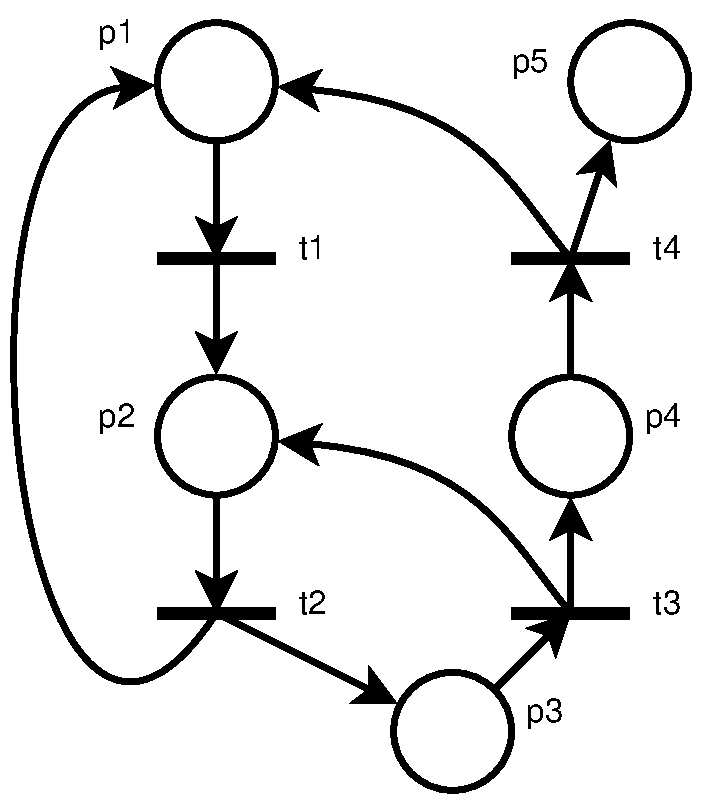
\includegraphics[width=0.3\textwidth]{Figures/EleccionSubredZonasInfluencia_1.eps}\end{matrix}
\ \ \ \ \ \ 
C=
\kbordermatrix{
   & t_1 & t_2 & t_3 & t_4\\
p_1& -1 &  1  &  0  &  1 \\
p_2&  1 & -1  &  1  &  0 \\
p_3&  0 &  1  & -1  &  0 \\
p_4&  0 &  0  &  1  & -1 \\
p_5&  0 &  0  &  0  &  1 \\
}
\]
We assume that we select as subnet the one formed by 4th and 5th places and transitions 1 and 2. Then the graph and the incidence matrix are thus:

\[
\begin{matrix}\includegraphics[width=0.50\textwidth]{Figures/subredInconexa.eps}\end{matrix}
\ \ \ \ \ \ 
C=
\kbordermatrix{
   & t_1 & t_2 & \vline & t_3 & t_4\\
p_4&  0 &  0  &  \vline & 1  & -1 \\
p_5&  0 &  0  &  \vline & 0  &  1 \\
\hline
p_1& -1 &  1  &  \vline & 0  &  1 \\
p_2&  1 & -1  &  \vline & 1  &  0 \\
p_3&  0 &  1  &  \vline & -1  &  0 \\
}
\]

Here we can see that although really $p_4 $, $ p_5 $, $ t_1 $ and $ t_2 $ are not isolated, there is no arc that connects them together. In the incidence matrix, the corresponding submatrix is the zero matrix. Therefore, whether or not there are elements isolated in the net, total subnet formed by $ p_4 $, $ p_5 $, $ t_1 $ and $t_2$ is a disjointed subnet.

\end{example}

We can extend this definition to a subnet that is part of a bigger net. It
doesn't matter in how many subnets it is separated: if one subnet is the null
matrix, this subnet is disjointed. This characteristic is implicit to the selected subnet and it doesn't depend on the rest of the net.

\subsubsection{Macroplace}

//TODO Introduccion
\begin{definition}[Macroplace]
A macroplace is a subnet that meets the following:
\begin{enumerate}
 \item arcs entering any node of the subnet from an external node come from a transition.
 \item arcs leaving any node on the subnet to an external node go to a transition.
\end{enumerate}
\end{definition}

\begin{proposition}
A subnet $N_1$ is a macroplace iif its transition influence matrix (TIM) is the null matrix. In the same way, $N_2$ is a macroplace iif its place
influence matriz (PIM) is the null matrix
\[
N_1\mbox{ is macroplace} \iff \forall a_{ij} \in TIM_1, a_{ij} =
0
\]
\[
N_2\mbox{ is macroplace} \iff \forall a_{ij} \in PIM_1, a_{ij} =
0
\]
\end{proposition}
TODO demostracion??

Suppose that the incidence matrix divided into the four pieces explained, $TIM$ appears to be the zero matrix. Then we conclude that the subnet $N_1$ is only related by arcs with places of subnet $N_2$. All arcs entering $N_1$ come from transitions of $N_2$ and all arcs coming out from $N_1$ go to transitions of $N_2$. Stated another way, the subnet $N_1$ behaves like a place, but may contain places and transitions.

Note that this is not really a place, and that the subnet has not marked as such. The marking is on the places within the subnet and depends on the arches of arrival.
\begin{example}[Macroplace]
//TODO
\end{example}

We can extend this definition to a subnet that is part of a bigger net too. However, in this time, it does matter the way in which the bigger net is separated. This characteristic is not implicit to the selected subnet and depends on the rest of the net.

//TODO explicar macroplace dependiendo del resto de subredes. Una subred puede comportarse como macrolugar sobre otra subred, pero no sobre una tercera.

//TODO macroplace absoluta si da igual el resto de subredes

//TODO Caracterizacion de macroplace absoluta

\subsubsection{Macrotransition}
\begin{definition}[Macrotransition]
A macrotransition is a subnet that meets with the following:
\begin{enumerate}
 \item arcs entering any node of the subnet from an external node come from a place.
 \item arcs leaving any node on the subnet to an external node go to a place.
\end{enumerate}
\end{definition}

\begin{proposition}
A subnet is a macrotransition iif its place influence matrix (PIM) is the null matrix.
\end{proposition}
//TODO demostracion??

This is other option that can happen is that in the incidence matrix: $PIM$ appears to be the zero matrix. Then we conclude that the subnet $N_1$ is only related by arcs with places of subnet $N_2$. All arcs entering $N_1$ come from places of $N_2$ and all arcs coming out from $N_1$ go to places of $N_2$. Stated another way, the subnet $N_1$ behaves like a transition, but may contain places and transitions.

Like macroplaces, macrotransitions are not transitions as such. It is not necessary that all entries are marked to fire the macrotransition, and not all output places are marked after entering it. Everything depends on the inner workings of the macrotransition.

\begin{example}[Macrotransition]
//TODO
\end{example}

We can extend this definition again to a subnet that is part of a bigger net too. Like with macroplaces, it does matter the way in which the bigger net is separated. 

//TODO explicar macrotransition dependiendo del resto de subredes. Una subred puede comportarse como macrotransition sobre otra subred, pero no sobre una tercera.

//TODO macrotransition absoluta si da igual el resto de subredes

//TODO Caracterizacion de macrotransicion absoluta

//TODO Explicar relacion entre una macrotransicion y un macrolugar en la
misma red, con subredes interrelacionadas por esta caracteristica. Una subred
es macrolugar sobre otra si y solo si esta ultima es macroplace sobre la
primera. Comprobarlo y demostrarlo en su caso

\begin{figure}[htbp]
\centering
\[
 \begin{matrix} 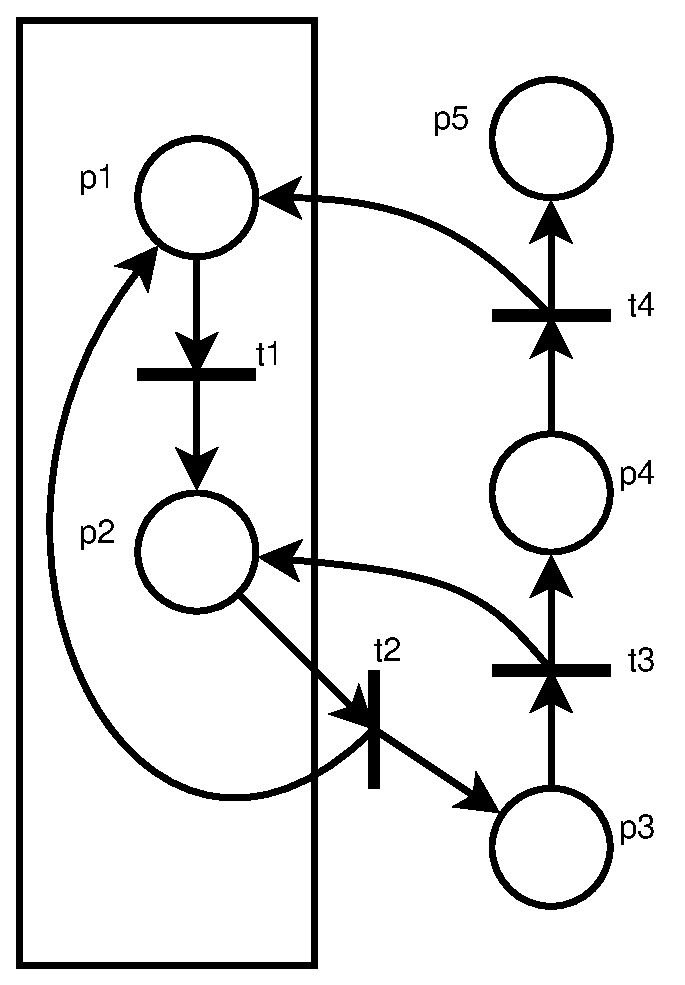
\includegraphics[width=0.32\textwidth]{Figures/macrolugar.eps}\\\mbox{a)
Macroplace}\end{matrix}
  \ \ \ \ \ \ \ \ \ \ \ \ \ \ \ \ 
 \begin{matrix}  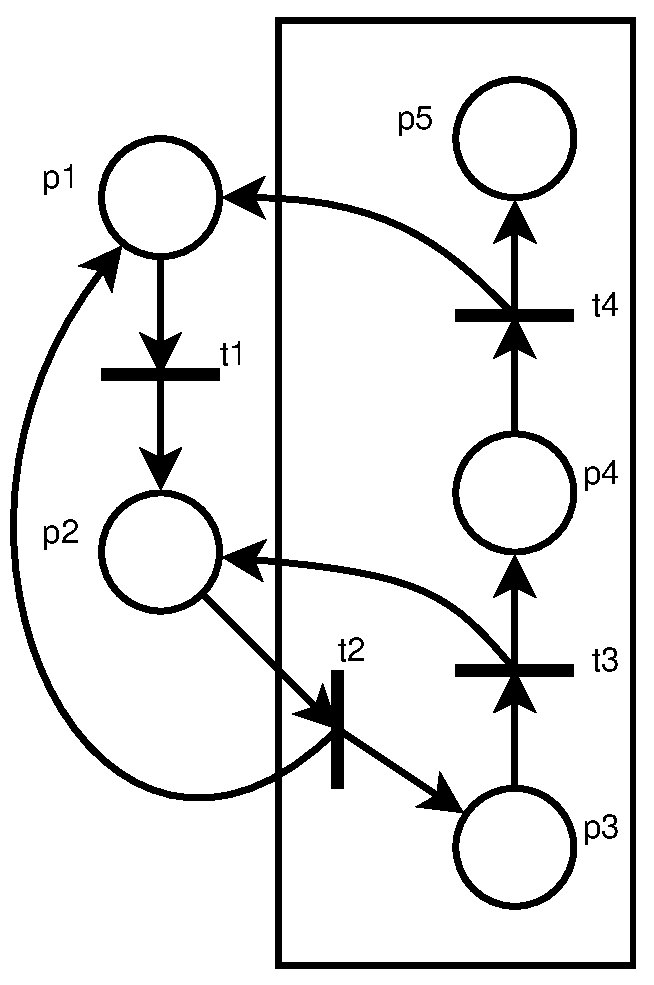
\includegraphics[width=0.3\textwidth]{Figures/macrotransicion.eps}\\\mbox{b)
Macrotransition}\end{matrix}
\]
\rule{35em}{0.5pt}
\caption{Macroplace y macrotransition //TODO quitar esta figura y poner en los
ejemplos de macrolugar y macrotransicion}
\label{fig:macrolugar_y_macrotransicion}
\end{figure}

\subsubsection{Sinkhole subnet}

Another thing that can happen is that the hidden subnet reach only arcs. We then find that you can not leave the subnet. We speak then of a sinkhole
subnet.

\begin{definition}[Sinkhole subnet]
It is said that a subnet is a sinkhole subnet if no arc has its origin in an internal node (place or transition) of the subnet.
\end{definition}

It is easy to see that a subnet is sinkhole if and only if all elements of $PIM$ are greater or equal to zero and all elements of $TIM$ are less than or equal to zero.
\[
N_1\mbox{ is sinkhole } \iff \forall a_{ij} \in PIM_{1}, a_{ij} \geq
0 \land \forall a_{pq} \in TIM_{1}, a_{pq} \leq 0
\]

//TODO demostracion??

\begin{example}[Sinkhole Subnet]
//TODO
\end{example}

If we can extend this definition to a subnet that is part of a bigger net,
in this case, it does matter the way in which the bigger net is separated. This characteristic is not implicit to the selected subnet and depends on the other subnets.

//TODO reescribir este parrafo anterior para que no sea
igual que los anteriores

//TODO explicar sinkhole dependiendo del resto de subredes. Una subred puede comportarse como sinkhole sobre otra subred, pero no sobre una tercera.

//TODO Sinkhole absoluta si da igual el resto de subredes

//TODO Caracterizacion de Sinhole subnet absoluta

\begin{figure}[htbp]
\centering
\[
 \begin{matrix}
    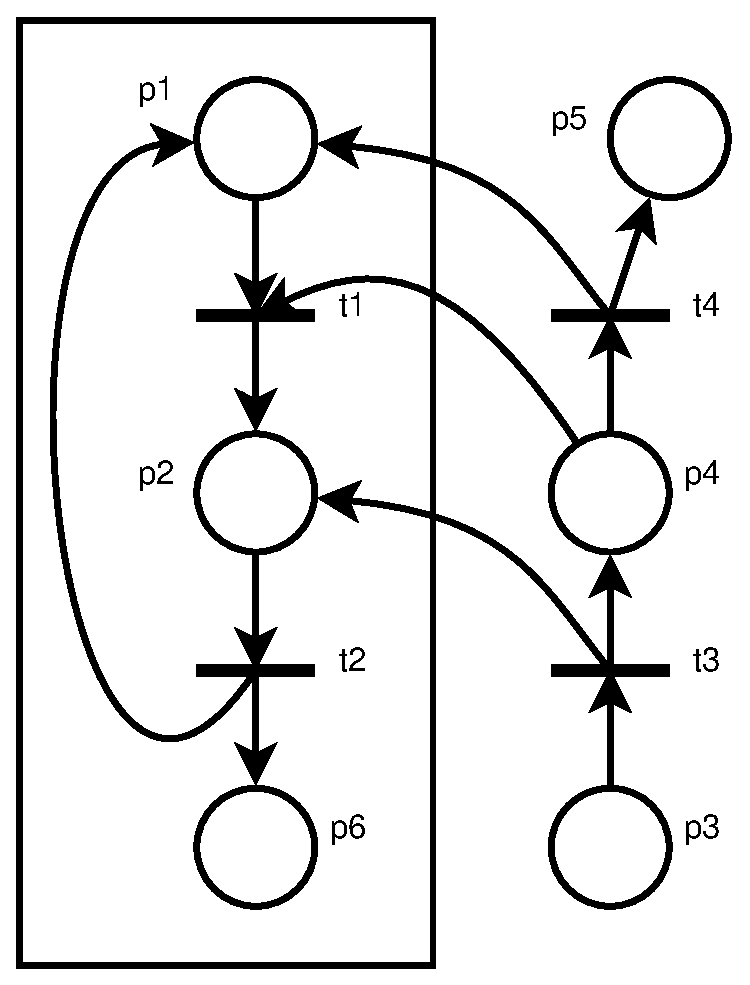
\includegraphics[width=0.3\textwidth]{Figures/subredSumidero.eps}
 \end{matrix}
  \ \ \ \ \ 
C=
\kbordermatrix{
   & t_1 & t_2 & \vline & t_3 & t_4\\
p_1&  -1 &  1  &  \vline & 0  & 1 \\
p_2&  1 &  -1  &  \vline & 1  &  0 \\
p_6&  0 &  1  &  \vline & 0  &  0 \\
\hline
p_3& 0 &  0  &  \vline & -1  &  0 \\
p_4&  -1 & 0  &  \vline & 1  &  -1 \\
p_5&  0 &  0  &  \vline & 0 &  1 \\
}
\]
\rule{35em}{0.5pt}
\caption{Sinkhole subnet}
\label{fig:subred_sumidero} 
\end{figure}


\subsubsection{Source subnet}
If instead of this what happens is no arc gets into the subnet, we have a source subnet. In a source subnet we can not enter.

\begin{definition}[Source subnet]
It is said that a subnet is a source subnet if no arc has its destination in an internal node (place or transition) of the subnet.
\end{definition}

\begin{figure}[htbp]
\centering
\[
 \begin{matrix}
    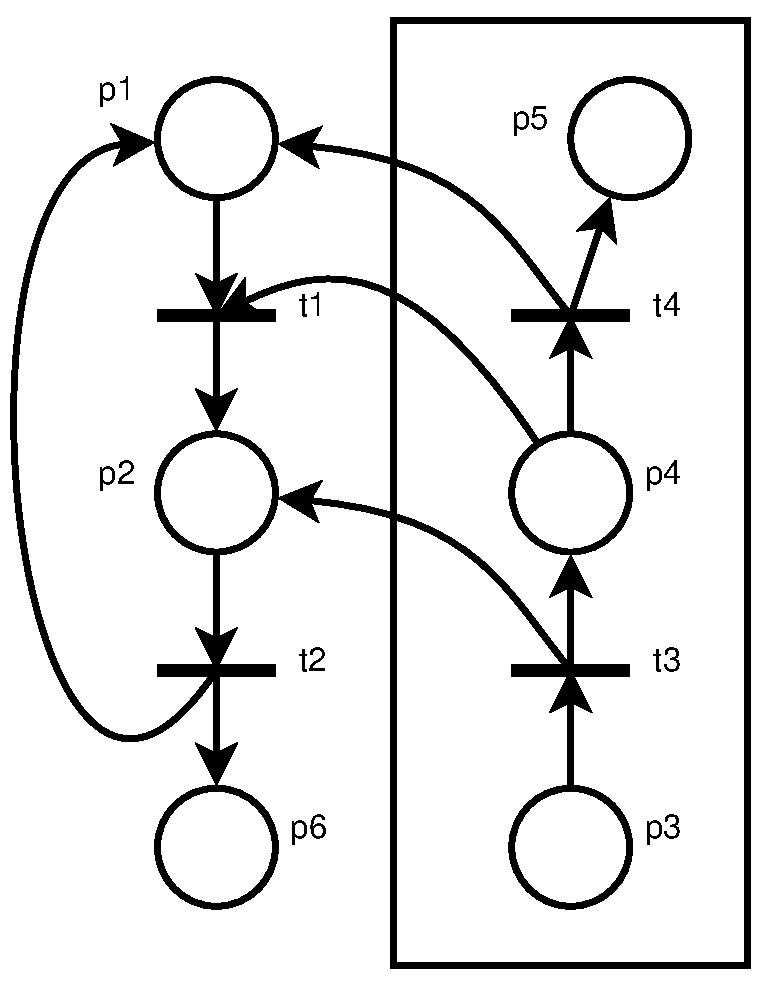
\includegraphics[width=0.3\textwidth]{Figures/subredFuente.eps}
 \end{matrix}
  \ \ \ \ \ 
C=
\kbordermatrix{
   & t_3 & t_4 & \vline & t_1 & t_2\\
p_3& -1 &  0  &  \vline & 0  &  0 \\
p_4&  1 & -1  &  \vline & -1  &  0 \\
p_5&  0 &  1  &  \vline & 0 &  0 \\
\hline
p_1&  0 &  1  &  \vline & -1  & 1 \\
p_2&  1 &  0  &  \vline & 1  &  -1 \\
p_6&  0 &  0  &  \vline & 0  &  1 \\
}
\]
\rule{35em}{0.5pt}
\caption{Source subnet}
\label{fig:subred_fuente} 
\end{figure}


It is easy to see that a subnet is source if and only if all elements of $TIM$ are greater than or equal to zero and all elements of $PIM$ are less than or equal to zero.
\[
\mbox{$N_1$ is source } \iff \forall a_{ij} \in TIM_1, a_{ij} \geq 0  \land \forall a_{pq} \in PIM_1, a_{pq} \leq 0
\]









\subsection{Matrix parts description once defined the subnets}

As places and transitions can be reordered smoothly, we study a network N divided into 2 subnets, for simplicity and without loss of generality.

For consistency with \cite{HID-Inigo2011MT} we will follow this notation:
\[
\left(
\begin{array}{c|c}
 H & HP\\
 \cline{1-2} 
 HT & V
\end{array}
\right)
\]
where
\begin{itemize}
\item H (Hidden Subnet) is the subnet wanted to be hidden.
\item V (Visible Subnet) is the subnet that is visible.
\item HT (Hidden Transitions Submatrix) are the relationships between places
of V and H transitions
\item HP (Hidden Places Submatrix) are the relations between transitions
of V and H sites
\end{itemize}

\begin{note}
Following this notation can be convenient because it is clear what is
each of the submatrices. However, elsewhere in the document be referenced as $ N_1 $ and $ N_2 $ for be more clarifying or being something generic and independent networks concealment. However, using $N_1 $ and $ N_2 $ the notation of subnets of influence with respect to the other is more diffuse.
\end{note}
\begin{figure}[htbp]
\centering
\[
 \begin{matrix} 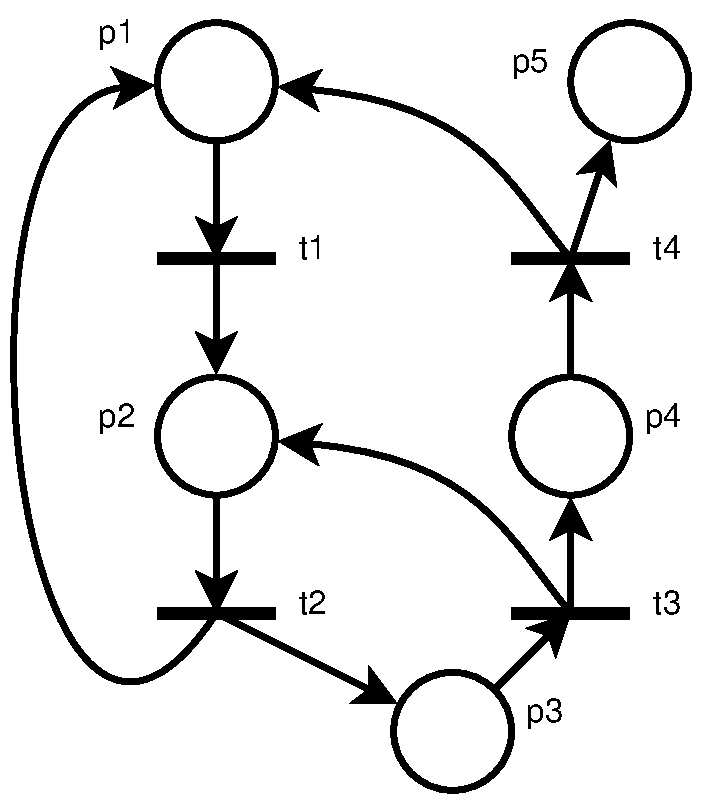
\includegraphics[width=0.3\textwidth]{Figures/EleccionSubredZonasInfluencia_1.eps}\end{matrix}
  \ \ \ \equiv \ \ \ 
 \begin{matrix}  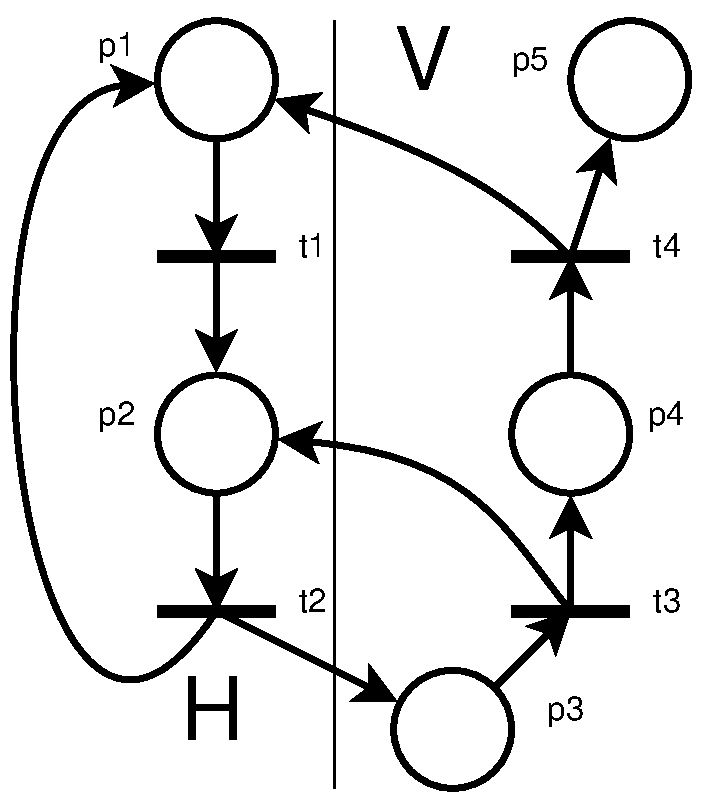
\includegraphics[width=0.3\textwidth]{Figures/EleccionSubredZonasInfluencia_2.eps}\end{matrix}
\]
\rule{35em}{0.5pt}
 \caption{Selecting subnet to hide}
 \label{fig:seleccion_subred_oculta} 
\end{figure}



\begin{example}
Consider the Petri net of the figure \ref{fig:seleccion_subred_oculta} with the next incidence matrix:
\[
\kbordermatrix{
   & t_1 & t_2 & t_3 & t_4\\
p_1& -1 &  1  &  0  &  1 \\
p_2&  1 & -1  &  1  &  0 \\
p_3&  0 &  1  & -1  &  0 \\
p_4&  0 &  0  &  1  & -1 \\
p_5&  0 &  0  &  0  &  1 \\
}
\]


The subnet we want to hide is formed by sites 1 and 2 and 1 and 2 transitions. Graphically, separate places and transitions to hide (H) from the rest of the network (V)

The incidence matrix is already sorted by the places and transitions to the top of it. Here are the four parts described above.
\[
\kbordermatrix{
   & t_1& t_2 & \vline &t_3 & t_4\\
p_1& -1 &  1  & \vline &  0  &  1 \\
p_2&  1 & -1  & \vline &  1  &  0 \\
\hline
p_3&  0 &  1  & \vline & -1  &  0 \\
p_4&  0 &  0  & \vline &  1  & -1 \\
p_5&  0 &  0  & \vline &  0  &  1 \\
}
\]

In this matrix we can see:
\begin{itemize}
  \item $H=\kbordermatrix{ & t_1 & t_2\\ p_1 & -1 & 1\\p_2 & 1 & -1\\}$
        is the subnet we want to hide. It is the same as $SN_1$
  \item $V=\kbordermatrix{&t_3&t_4\\p_3&-1&0\\p_4&1&-1\\p_5&0&1\\}$ is the
        subnet that is visible. It is the same as $SN_2$
  \item $HP=\kbordermatrix{ & t_3 & t_4\\ p_1 & 0 & 1\\p_2 & 1 & 0\\}$ are
        the relationships between transitions of V and H places. It is the
        equivalent to $PIM_1$ or $TIM_2$
  \item $HT=\kbordermatrix{&t_1&t_2\\p_3&0&1\\p_4&0&0\\p_5&0&0\\}$ are
        the relationships between places of V and H transitions. It is the
        equivalent to $TIM_1$ or $PIM_2$
\end{itemize}
\end{example}

At this moment, it is easy to see that we can choose any subset of places
and transitions in order to hide it, simply reordering rows and columns.

\begin{example}
In the previous example we have seen a fairly simple option selection
subnet and we have chosen the locations 1 and 2 and the transitions 1 and
2. However, we can choose any other subset of places and transitions.
In this example we will select locations 2, 3 and 5 and the transitions
1 and 3. Thus, in the graph of the previous example move the locations and transitions to hide on one side and the rest on the other.
\begin{center}
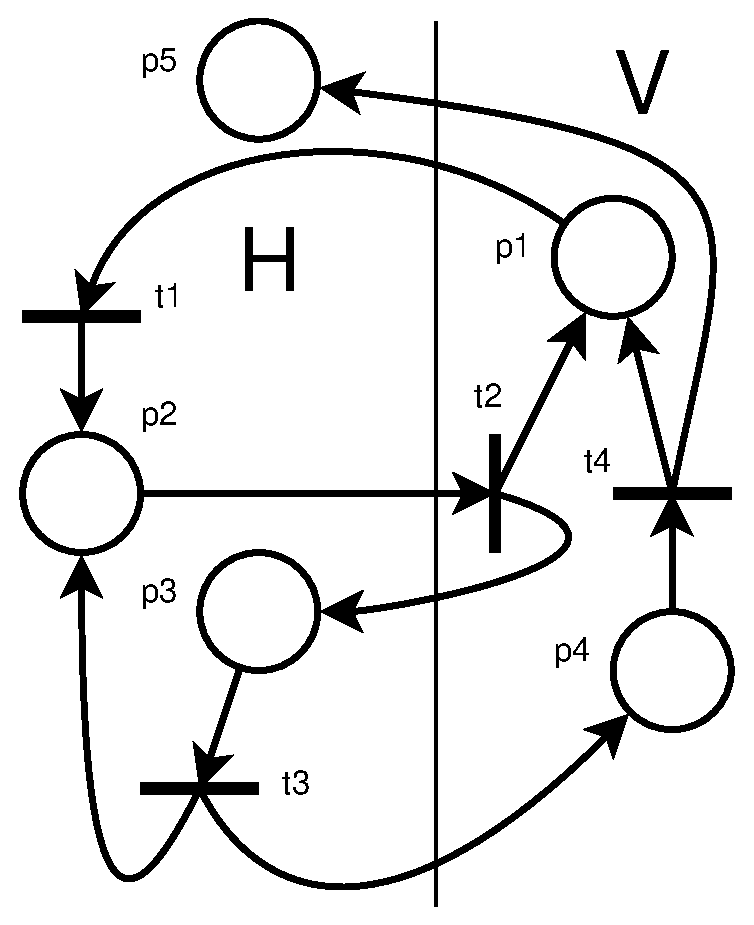
\includegraphics[width=0.3\textwidth]{Figures/EleccionSubredZonasInfluencia_3.eps}
\end{center}
Although more confusing, can be seen that the graph is the same as the incidence matrix is the same (not just part of the equivalence class, it is exactly the same). Now, in this matrix move places 2, 3 and 5, and 1 and 3 transitions at the beginning of the matrix:
\[
\kbordermatrix{
   & t_1& t_3 & \vline &t_2 & t_4\\
p_2&  1 &  1  & \vline & -1  &  0 \\
p_3&  0 & -1  & \vline &  1  &  0 \\
p_5&  0 &  0  & \vline &  0  &  1 \\
\hline
p_1& -1 &  0  & \vline &  1  &  1 \\
p_4&  0 &  1  & \vline &  0  & -1 \\
}
\]

Interpreting each of the chunks of the matrix is similar to the previous example.
\end{example}

\subsection{Private information. Hiding a subnet}

Once you select the private subnet we proceed to the occultation
as such \cite{HID-Inigo2011MT}. Graphically, it seems simple. Just replace the subnet to hide by a black box and modify some arcs according to the following
rules:

\begin{enumerate}
\item The arcs originating in a place or transition within the black box, and target a place or transition out of it will have the black box as the source.
\item The arcs originating in a place or transition out of the black box, and target a place or transition within it, are replaced by the black box as a destination.
\end{enumerate}

\begin{example}
We consider the Petri net of the  Figure \ref{fig:seleccion_subred_oculta}.
The result of hiding the part of the graph H is the following:
\[
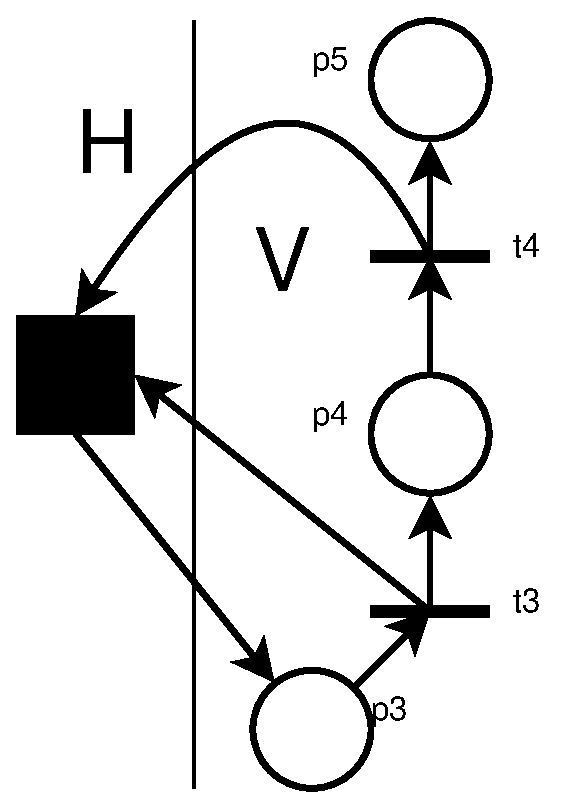
\includegraphics[width=0.3\textwidth]{Figures/OcultacionSubred_1.eps}
\]
\end{example}

In the associated incidence matrix also replace the H elements by a black box:
\[
\kbordermatrix{
   & t_1 &  t_2 & \vline &t_3 & t_4\\
p_1& \rule{0.15in}{0.15in} & \rule{0.15in}{0.15in}    & \vline &  0  &  1 \\
p_2& \rule{0.15in}{0.15in} & \rule{0.15in}{0.15in}   & \vline &  1  &  0 \\
\hline
p_3&  0 &  1  & \vline & -1  &  0 \\
p_4&  0 &  0  & \vline &  1  & -1 \\
p_5&  0 &  0  & \vline &  0  &  1 \\
}
\]

However, in this matrix notation is given information should also be hidden: it gives us information about the number of places and transitions of the hidden subnet, besides indicating hidden places and transitions with which it interacts. To solve this problem we proceed as follows. We can group all rows for the screened subnet into one. In each row position examine all elements of the original rows corresponding to that position, and will put:

\begin{itemize}
\item If all these elements are zero, in the grouped row will be a zero.
\item If one and only one of those elements is nonzero, will put that item.
\item If there are several non-zero elements, we will post a list of these items separated by commas, creating a d-dimensional element (in $ d $ dimensions).
\end{itemize}

In the same way we have done with the rows, proceed with columns. Thus, if the hidden subnet has $ i $ columns and $ j $ rows, we will get a matrix
like this:
\[
\left(
\begin{array}{c|ccc}
 \rule{0.15in}{0.15in} & a_{1(i+1)} & \cdots & a_{1m} \\
 \cline{1-4} 
 a_{(j+1)1} & &   & \\
 \vdots & & V & \\
 a_{n1} & &   & \\
\end{array}
\right)
\]

where $\forall p, \forall q |  i+1\le p \le m \land j+1\le q \le n$
\[
a_{1p}=\left\{ \begin{array}{ll}
0 & \mbox{ if }\forall r | 1 \le r \le j, c_{rp}=0\\
c_{rp}& \mbox{ if } \exists! r, 1 \le r \le j | c_{rp}\neq0\\
(c_{r_1p}, c_{r_2p},...) & \mbox{ if }\exists r_1\neq r_2 \neq ..., 1 \le r_1, r_2,... \le j\\& |c_{r_1p},c_{r_2p},...\neq0
\end{array}\right.
\]
\[
a_{q1}=\left\{ \begin{array}{ll}
0 & \mbox{ if }\forall s | 1 \le s \le i, c_{qs}=0\\
c_{qs}& \mbox{ if } \exists! s, 1 \le s \le i | c_{qs}\neq0\\
(c_{qs_1}, c_{qs_2},...) & \mbox{ if }\exists s_1\neq s_2 \neq ..., 1 \le s_1, s_2,... \le s\\& |c_{qs_1},c_{qs_2},...\neq 0
\end{array}\right.
\]

So we hide the number of places and transitions of the hidden subnet
and their relationships.
Yes, some information is given about the hidden network. Really if this resulting matrix some node that is d-dimensional, at least in the hidden network must exist $ d $ nodes of this type.
\begin{example}
We consider the Petri net defined by the following incidence matrix, separated into $H$,$V$,$HT$ and $HP$.
\[
\left(
\begin{array}{ccc|ccc}
-1 & 0 & 1 & 0 & 0 & 0\\
-1 & 0 & 0 & 1 & 0 & 1\\
1 & 0 & 0 & -1 & 0 & 0\\
1 & -1 & 0 & 1 & 0 & 0\\
\hline
0 & 1 & 0 & 0 & 0 & 0\\
1 & 0 & -1 & 0 & 0 & 0\\
0 & 0 & 0 & -1 & -1 & 1\\
0 & 0 & 0 & 0 & 1 & -1\\
\end{array}
\right)
\]

After applying the above steps for the group, we would have the following:
\[
\left(
\begin{array}{c|ccc}
\rule{0.15in}{0.15in} & (1,-1,1) & 0 & 1\\
\hline
1  & 0 & 0 & 0\\
(1,-1) & 0 & 0 & 0\\
0 &  -1 & -1 & 1\\
0 &  0 & 1 & -1\\
\end{array}
\right)
\]

Here we see that the information about the number of hidden places and transitions is minimized. So we know that at least there are two hidden transitions and at least three hidden places (there is a transition of dimension 3). However, we do not know the exact number of either.
\end{example}

 

\subsection{Front-end interaction with the subnet. Input and output functions}

Once you have defined all this environment, we will try to go a little further. Let's assume that we want to export a subnet we have hidden in another network, like a black box. Our intention is to connect this hidden network to another network, and can thus be reused subnets. For example, let's assume that we have a process modeling with Petri net modeling and in this there is a subnet we want to hide, but, at the same time, we want to reuse it in other Petri nets.

In this case we have a problem, and once hidden network disappears half the information input or output arcs of the same. In particular, we do not know the source nodes and arcs that leave the target nodes of the arcs that enter the network until no visible again. But if we want to reuse it on other networks, can not wait to make it visible. Should remain hidden, but should be able to connect to other networks.

We will try to solve this problem. This way we can reuse hidden networks like plug-in modules on other networks. However, we will not need the actual implementation of the source or destination nodes of the arcs that leave or enter the network, respectively. The solution is to define a facade or front-end input and output of the network. This front-end will contain the information needed to interact with the network hidden, but hide the specifics of implementation. To define this behavior going from some assumptions.

\subsubsection{Previous definitions}

Let $R=\langle P,T,\alpha,\beta\rangle$ be a Petri net and let $P=\{R_1,
R_2\}$ be a partition of $R$. 

\begin{definition}[Input place]
Let $p_i$ a place of $R_1$. $p_i$ is an input place of $R_1$ if it is the
destination of an arc coming from a $R_2$ transition, ie,
\[
p_i \mbox{ is an input place of } R_1 \mbox{ if } \exists t_j \in R_2\ | c_{ij}>0
\]
\end{definition}

\begin{definition}[Input transition]
Let $t_i$ a transition of $R_1$. $t_i$ is an input transition of $R_1$ if it is the destination of an arc coming from a $R_2$ place, ie,
\[
t_i \mbox{ is an input transition of } R_1 \mbox{ if } \exists p_j \in R_2 | c_{ji}<
0
\]
\end{definition}

\begin{definition}[Input node]
An input node of $R_1$ is an input place or transition of $R_1$.
\end{definition}

\begin{definition}[Output place]
Let $p_i$ be a place of $R_1$. $p_i$ is an output place of $R_1$
if an arc leaves it towards a transition of $R_2$, ie,
\[
p_i \mbox{is an output place of } R_1 \mbox{ if } \exists t_j \in R_2 | c_{ij} < 0
\]
\end{definition}

\begin{definition}[Output transition]
let $t_i$ be a transition of $R_1$. $t_i$ is an output transition of $R_1$ if an arc leaves it towards a place of $R_2$, ie,
\[
t_i \mbox{ is an output transition of } R_1 \mbox{ if } \exists p_j \in R_2 | c_{ji} > 0
\]
\end{definition}

\begin{definition}[Output node]
An output node of $R_1$ is an output place or transition of $R_1$.
\end{definition}

After defining these concepts, we can define the sets thereof.

\begin{notation}
We denote the sets of the elements defined above:
 \begin{shortitemize}
  \item Let $IP(R) \subseteq  \overline P$ (Input Places) be the set of input  places of a subnet.
  \item Let $IT(R) \subseteq \overline T$ (Input Transitions) be the set of input transitions of a subnet.
  \item Let $IN(R) \subseteq \overline P \cup \overline T$ (Input Nodes)
        be the set of input nodes of a subnet.
  \item Let $OP(R) \subseteq  \overline P$ (Output Places) the set of output places of a subnet.
  \item Let $OT(R) \subseteq \overline T$ (Output Transitions) be the set of output transitions of a subnet.
  \item Let $ON(R) \subseteq \overline P \cup \overline T$ (Output Nodes)
        be the set of output nodes of a subnet.
\end{shortitemize}
\end{notation}

\begin{note}
Recall that a node in a Petri net can be both a place and a transition, depending on the context.
\end{note}
\begin{notation}
Denote as $ n_i $ to a node of a Petri net.
\end{notation}

\begin{figure}[htbp]
\centering
\[
 \begin{matrix} 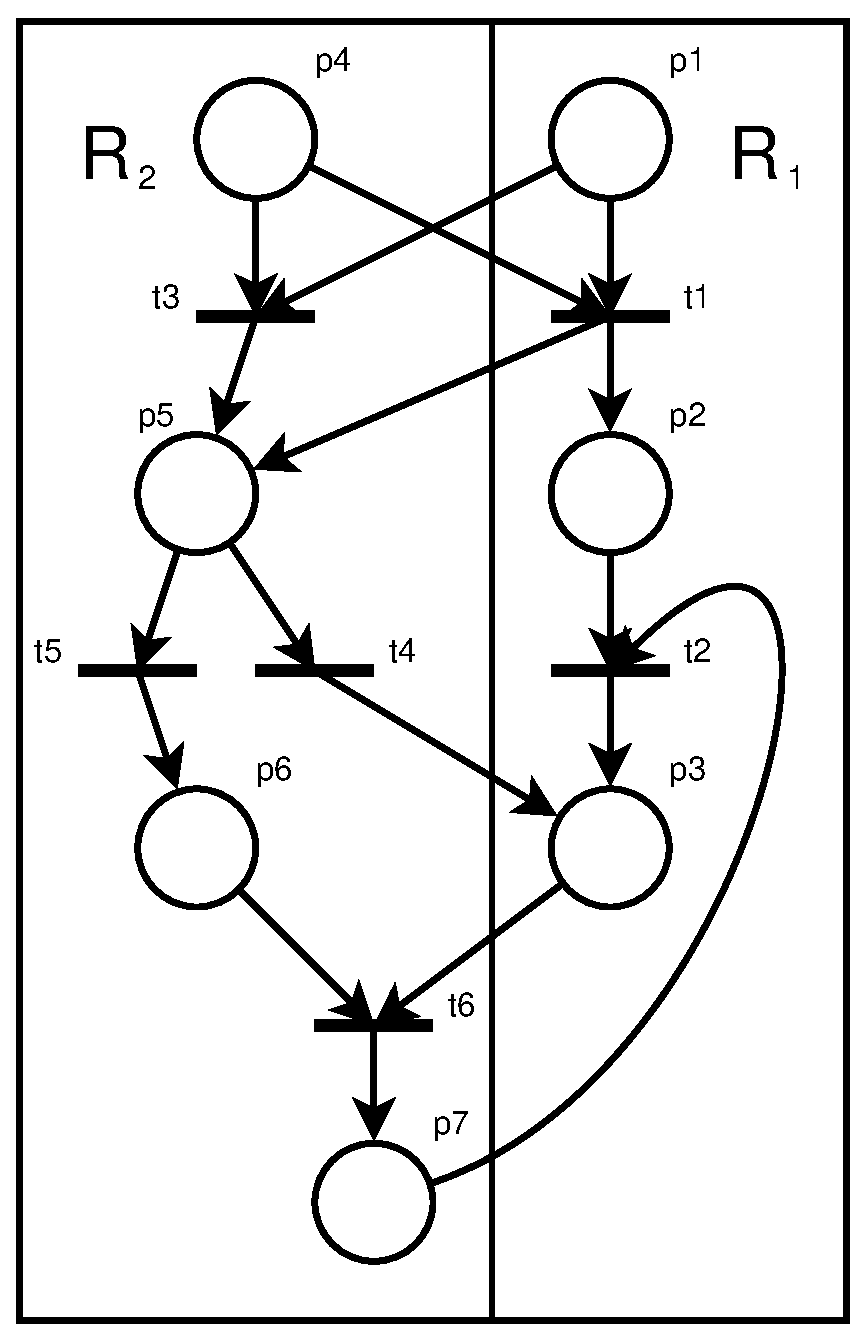
\includegraphics[width=0.3\textwidth]{Figures/NodosEntradaSalidaV.eps}\end{matrix}
  \ \ \ \ \ 
C=
\kbordermatrix{
   & t_1 & t_2 & \vline & t_3 & t_4 & t_5 & t_6\\
p_1& -1 &  0  &  \vline & -1  &  0 & 0  &  0 \\
p_2&  1 & -1  &  \vline & 0  &  0 & 0  &  0 \\
p_3&  0 &  1  &  \vline & 0 &  1 & 0  &  -1 \\
\hline
p_4&  -1 &  0  &  \vline & -1  & 0 & 0  &  0 \\
p_5&  1 &  0  &  \vline & 1  &  -1 & -1  &  0 \\
p_6&  0 &  0  &  \vline & 0  &  0 & 1  &  -1 \\
p_7&  0 &  -1  &  \vline & 0  &  0 & 0  &  1 \\

}
\]
\rule{35em}{0.5pt}
\caption{Subnets with input and output nodes}
\label{fig:nodos_entrada_salida} 
\end{figure}


As we have generic definitions, no problem in applying to a network divided into $ H $, $ V $, $ HN $ and $ HT $, as the set $ \{H, V \} $ is a partition of $ R $.

\subsubsection{Subnet Front-end}

Once all these concepts, we create the front-end input/output of a Petri subnet. A front-end of the Petri net will be a intermediate facade that allows us to physically divide that subnet from the rest of the net. Thus, in order to enter or leave the subnet, you need to make it through this front-end.

Let $ IA $ (input arcs) the set of arcs that enter the subnet $ R_1 $ and let $ OA $ (output arcs) the set of arcs leaving $ R_1 $.

\begin{definition}[Input gate of a net]
Let $ a_i \in IA $ an arc of entrance to $ R_1 $. We define an input gate to $ R_1 $, and denote by $ ig_i $, as a new logical node that is identified with an arc of entrance to the net. For each input arc, defines an input gate, regardless of the origin and destination of the arc. If the source is a transition, we denote $ igt_i $ and if a place, $ igp_i $.
\end{definition}

\begin{definition}[Output gate of a net]
Let $ a_i \ in OA $ output arc $ R_1 $. We define an output gate of $ R_1 $, and denote by $ og_i $, as a new logical node that is identified with an exit arc of the net. For each exit arc is defined an output gate, regardless of the origin and destination of the arc. If the source is a transition, we denote $ ogt_i $ and if it is a place, $ ogp_g$.
\end{definition}

In this way we can divide the input arcs and output into two parts: a $ R_1 $ internal and external to $ R_1 $. If we take an arc of entrance $ a_i $ that has an origin in $n_j $ and destination
in $ n_k $, we define an input gate through a point of entry so that the original arc $ a_i $ is divided into two parts.
\begin{itemize}
  \item $a_{i1}$ (external to $R_1$) with origin in $n_j$ and destination  in $igt_i$ or $igp_i$ depending on if $n_j$ is a transition or a place.
  \item $a_{i2}$ (internal to $R_1$) with destination in $igt_i$ or $igp_i$ depending on if $n_j$ is a transition or a place respectively.
\end{itemize}

Similarly, if we take a exit arc $ a_i $ that has an origin in $ n_k $ and destination in $ n_j $, we define an output gate $ og_i $ so that the original arc $ a_i $ is divided into two parts:
\begin{itemize}
  \item $a_{i1}$ (internal to $R_1$) with origin in $n_k$ and destination
  in $igt_i$ or $igt_i$ depending on if $n_j$ is a transition or a place
.
  \item $a_{i2}$ (external to $R_1$) with destination in $n_j$ and origin
  in $igt_i$ or $igp_i$ depending on if $n_j$ is a transition or a place
  respectively. 
\end{itemize}

\begin{example}
\label{ej:puertas_entrada_salida}
Consider the net in figure \ref{fig:nodos_entrada_salida}. In this network we have three arcs entering and leaving three arcs. For each of those emerging define output gates and each coming, we define input gates. The subnet $ R_1 $ becomes:
\[
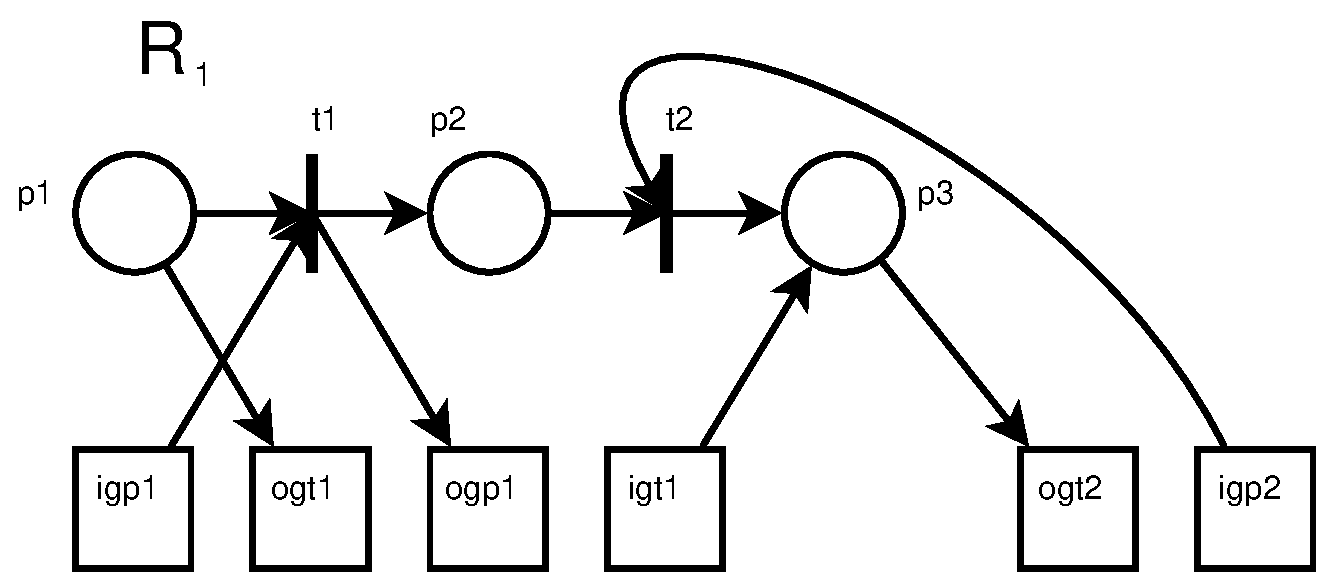
\includegraphics[width=0.7\textwidth]{Figures/PuertasEntradaSalida_1.eps}
\]
and in the complete net, arcs entering and leaving are divided into two pieces:
\[
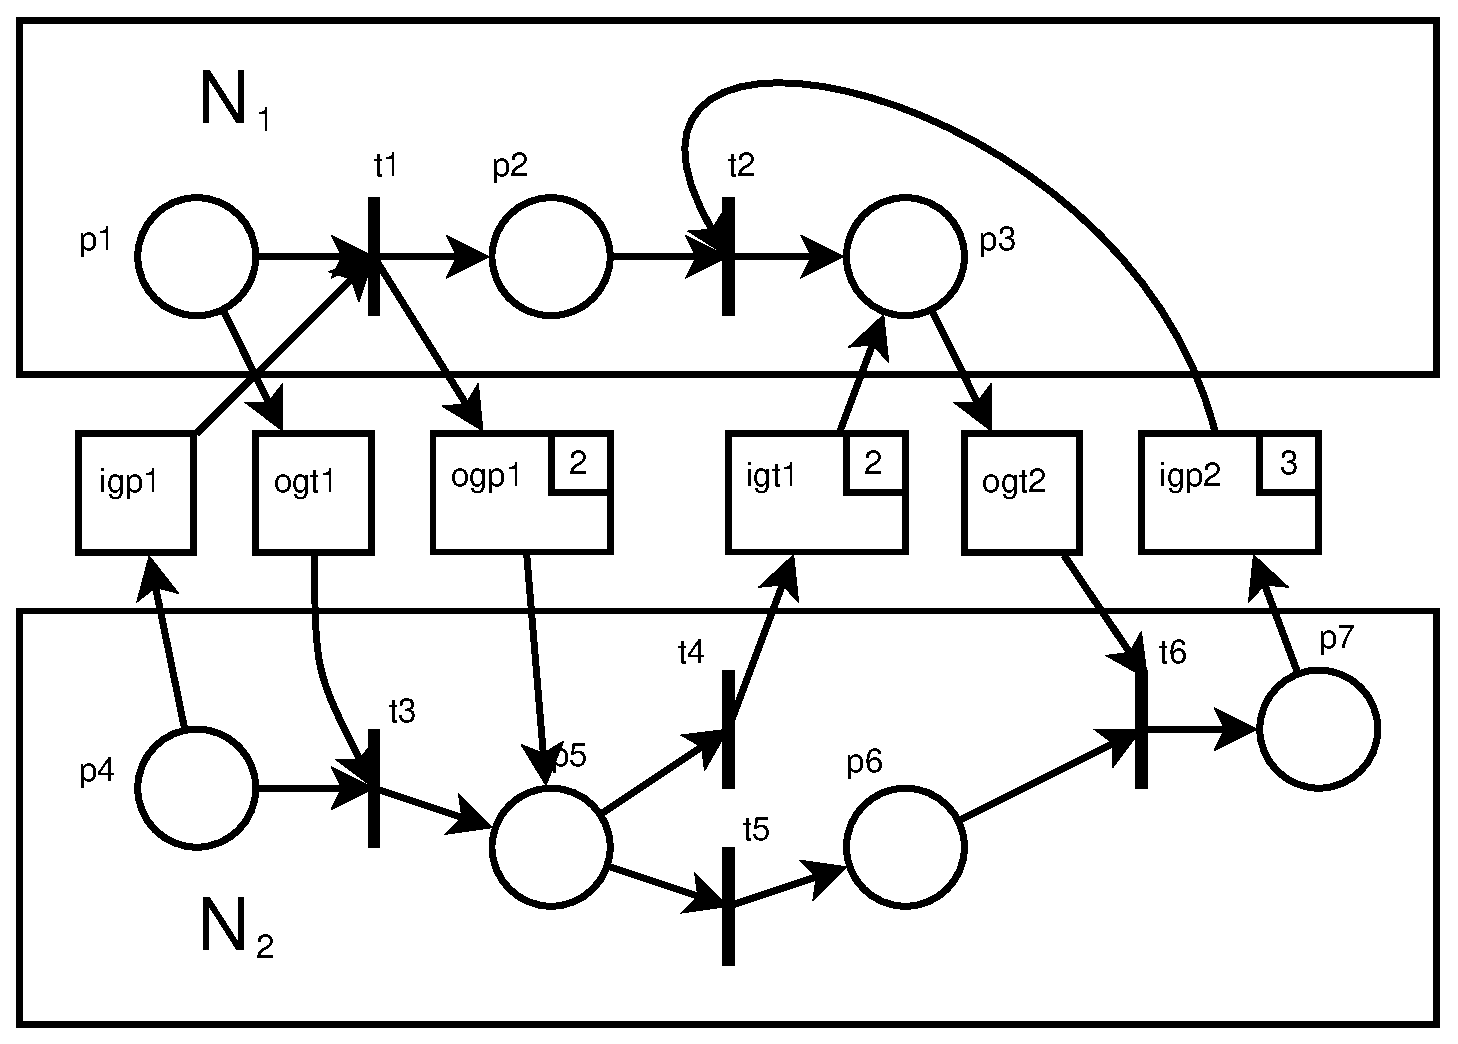
\includegraphics[width=0.7\textwidth]{Figures/PuertasEntradaSalida_2.eps}
\]
\end{example}

\begin{definition}[Input Front-end of a net]
The input front-end (or input interface) of a subnet $R_1$ is the set of all input gates of $ R_1 $. We denote by $ IF $ of $ R_1 $.
\end{definition}

\begin{definition}[Output Front-end of a net]
The output front-end (or output interface)of a subnet $R_1$ is the set of all output gates of $ R_1 $. We denote by $ OF $ of $ R_1 $.
\end{definition}

\begin{definition}[Front-end of a net]
The front-end (or interface) of a net $R_1$ is the pair of $IF$ and $OF$ of $R_1$. We denote by $ F $ of $ R_1 $.
\[
F = \langle IF, OF\rangle
\]
\end{definition}

\begin{example}
Taking the net of the example \ref{ej:puertas_entrada_salida} and applying these new definitions, we would have $ R_1 $ net along with its front end as shown in Figure \ref{fig:front-end}.
\end{example}

\begin{figure}[htbp]
\centering
\[
 \begin{matrix} 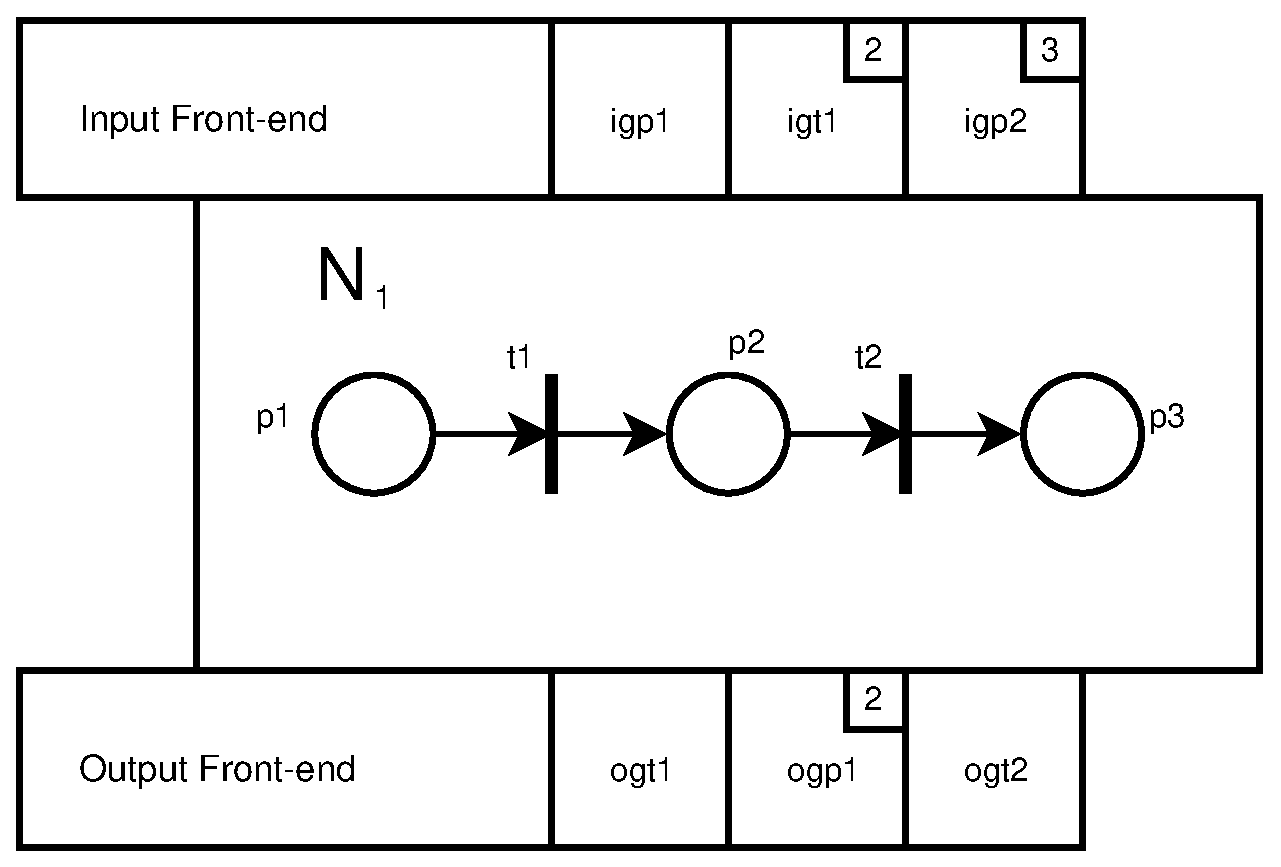
\includegraphics[width=0.5\textwidth]{Figures/Front-endEnglish.eps}\end{matrix}
\]
\rule{35em}{0.5pt}
 \caption{Front-end of a net}
 \label{fig:front-end} 
\end{figure}

//TODO estudiar mas en profundidad la relacion entre la matriz con filas
y columnas agrupadas. La fila y columna ocultas indican puertas de entrada/salida a la subred.

\subsubsection{Input/output functions}

Once all these input and output concepts defined, we will introduce a few key concepts for our purpose.

Let $ R $ a Petri net and let $ \{R_1, R_2 \} $ a partition of $ R $. Let $ F = \langle IF, OF \rangle $ the front-end of $ R_1 $.

\begin{definition}[Petri net Input function]
 We define the input function $f_i$ of $R_1$ as:
\[
  f_i:F \longrightarrow IN
\]
such that for each input gate $ igt_i$ you mapped one or no input place $ R_1 $ and each input gate $ igp_j$ you mapped one or no input transition $ R_1 $. 

\end{definition}

\begin{definition}[Petri net Output function]
We define the output function $f_o$ of $R_1$ as:
\[
  f_o:ON \longrightarrow F
\]
such that each output place $ R_1 $ you mapped one or no output gate $ ogt_i $ of $ R_1 $ and each output transition $ R_1 $ you mapped one or no output gate $ ogp_j $ to $ R_1$
\end{definition}

The input function can be defined for all the input gates and the output function should be surjective because if not, some door would not be connected. Anyway that is not essential. If a front-end door is not connected with any element of your network, simply by solving the final network, the arcs connected to that door disappear. Note also that the input function is not necessarily injective: Multiple input gates can be associated to the same node of $ R_1 $.

\begin{example}
Consider the net $ R_1 $ in figure \ref{fig:nodos_entrada_salida} with its front-end in figure \ref{fig:front-end}. The input and output functions are:

\begin{itemize}
\item Input function: 
$
\begin{array}{c|ccc}
F & igp_1 & igt_1 & igp_2\\
\hline
IN & t_1 & p_3 & t_2\\
\end{array}
$
\item Output function: 
$
\begin{array}{c|ccc}
ON & p_1 & t_1 & p_3\\
\hline
F & ogt_1 & ogp_1 & ogt_2\\
\end{array}
$
\end{itemize}
\end{example}

//TODO peso de los arcos y colores

\subsubsection{Attachable net}

By joining the subnet $ R_1 $ along with its front-end and its input and output functions $ f_i $ and $ f_o $ we grouped both the internal network with external communication. This way we can '' extract'' a subnet and ''implant'' it in another net. You only need this destination network is to communicate with the front-end. So naturally appears the following definition.

\begin{definition}[Attachable Petri net]
An Attachable Petri net is a quadruple $R_a=\langle R,F,f_i,f_o\rangle$
\end{definition}

From these definitions, it is clear that you can create attachable subnets taking a subnet of another given and applying the whole process we have defined. But it is also possible to create from scratch, starting from a network, defining a front end for that network and declaring the input and output functions. So you can create Petri nets modules providing functionality and out through a front-end without requiring the actual implementation.

\begin{example}
The attachable net in figure \ref{fig:nodos_entrada_salida} would be the
next:
\[
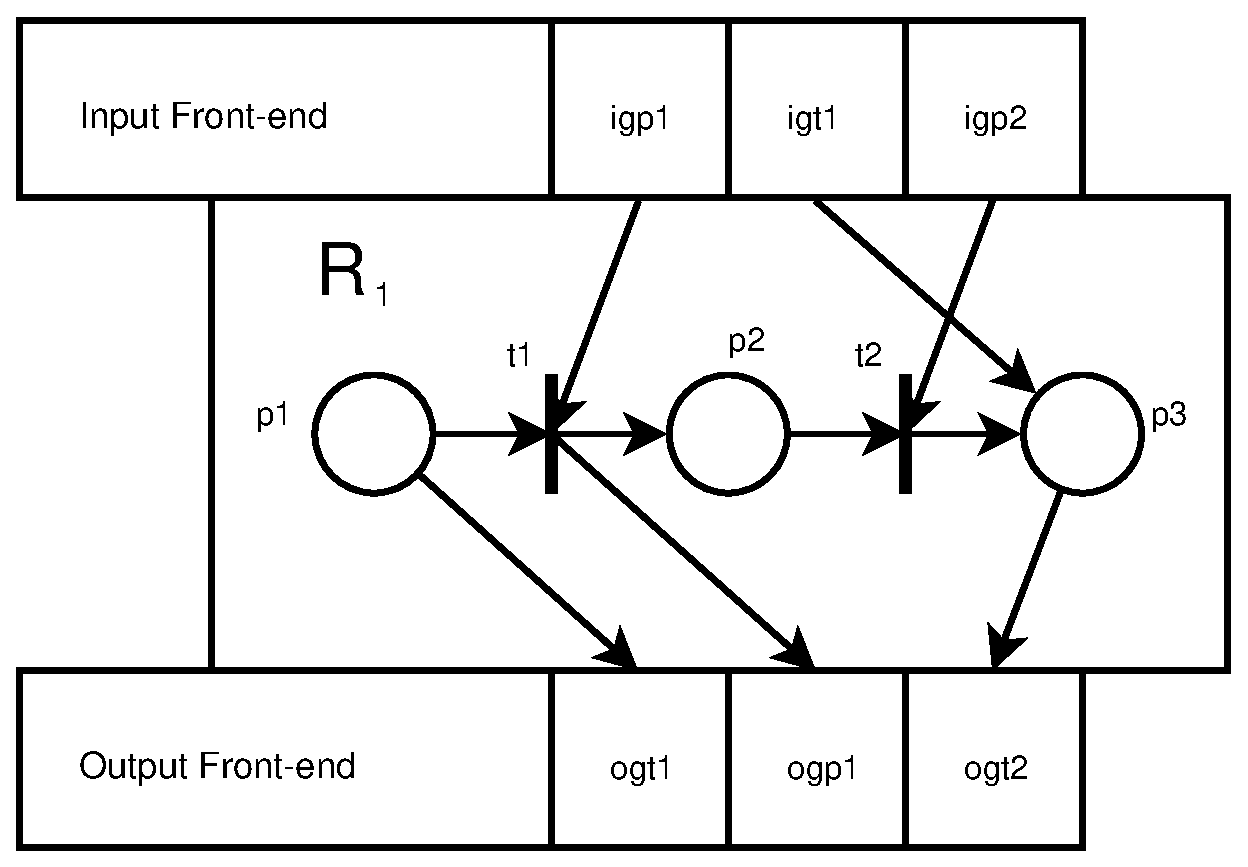
\includegraphics[width=0.5\textwidth]{Figures/RedAcoplable_1English.eps}
\]
\end{example}
It can be seen as a private black box with visible input and output connectors that are ''plugged'' to other networks. In a attachable net, the private part would be $ R $, $ f_i $ and $ f_o $. The public part of the front-end would be $ F $. All a net need to know is the input/output front-end.

A utility of these nets is that its definition is simple, since only the front-end is needed to define its operation. This makes possible to create nets using attachable nets in certain areas where they do not know their actual implementation, but its behavior. Additionally, it is possible to use different implementations of ''network providers'' of the same attachable nets, using at each moment the most appropriate one.

\begin{example}
Consider now the following Petri net
\[
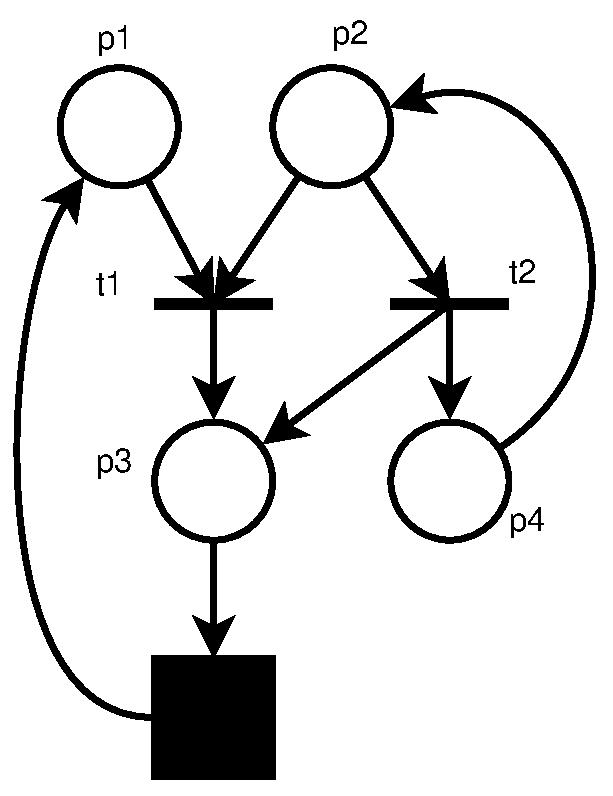
\includegraphics[width=0.3\textwidth]{Figures/RedAcoplable_2.eps}
\]
to which we want to connect an attachable net in the black box. Let's assume we have two equivalent alternatives described in Example \ref{ej:ocultacion_reduccion}:
\[
 \begin{matrix} 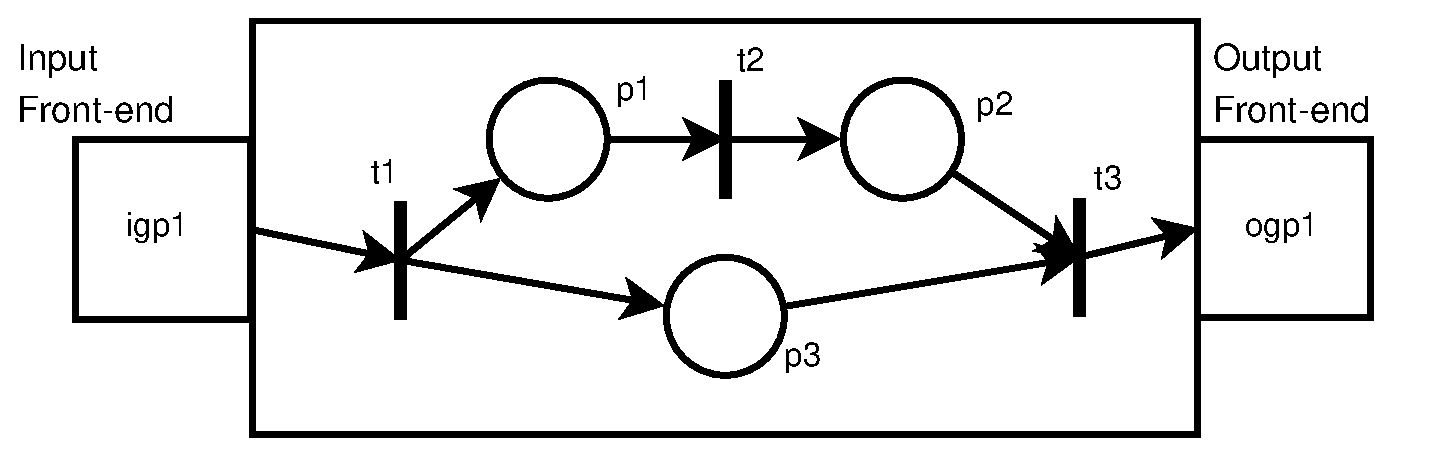
\includegraphics[width=0.6\textwidth]{Figures/RedProveedor_1English.eps}\end{matrix}
\]
\[
 \begin{matrix}  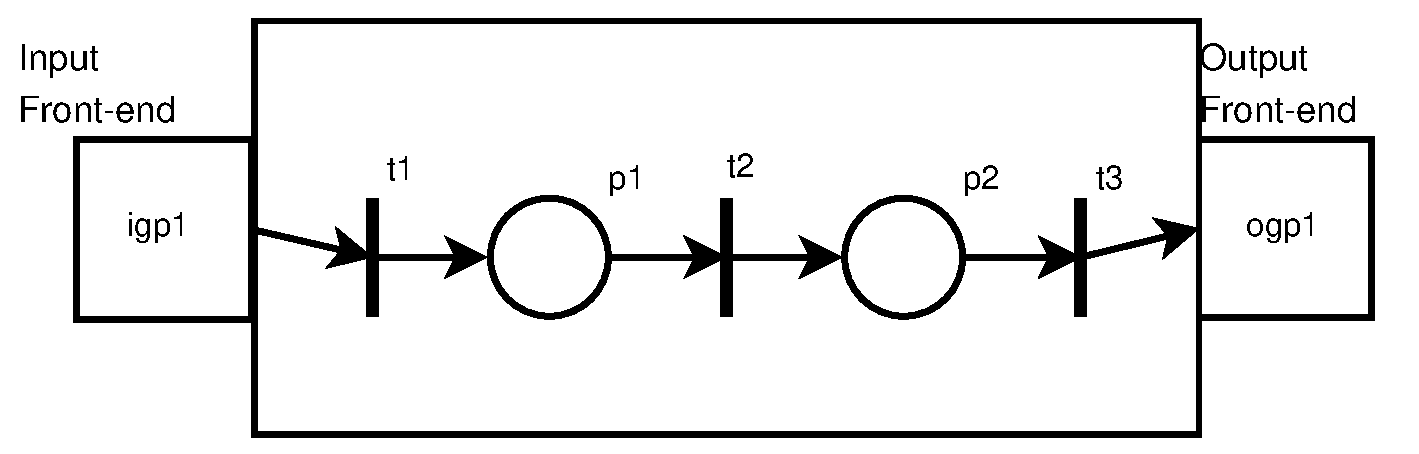
\includegraphics[width=0.6\textwidth]{Figures/RedProveedor_2English.eps}\end{matrix}
\]

We Can ''plug'' either because their front ends are equivalent and remains in figure \ref{fig:redes_acoplables}.



\begin{figure*}[htbp]
\centering
\[
 a) \ \ 
 \begin{matrix} 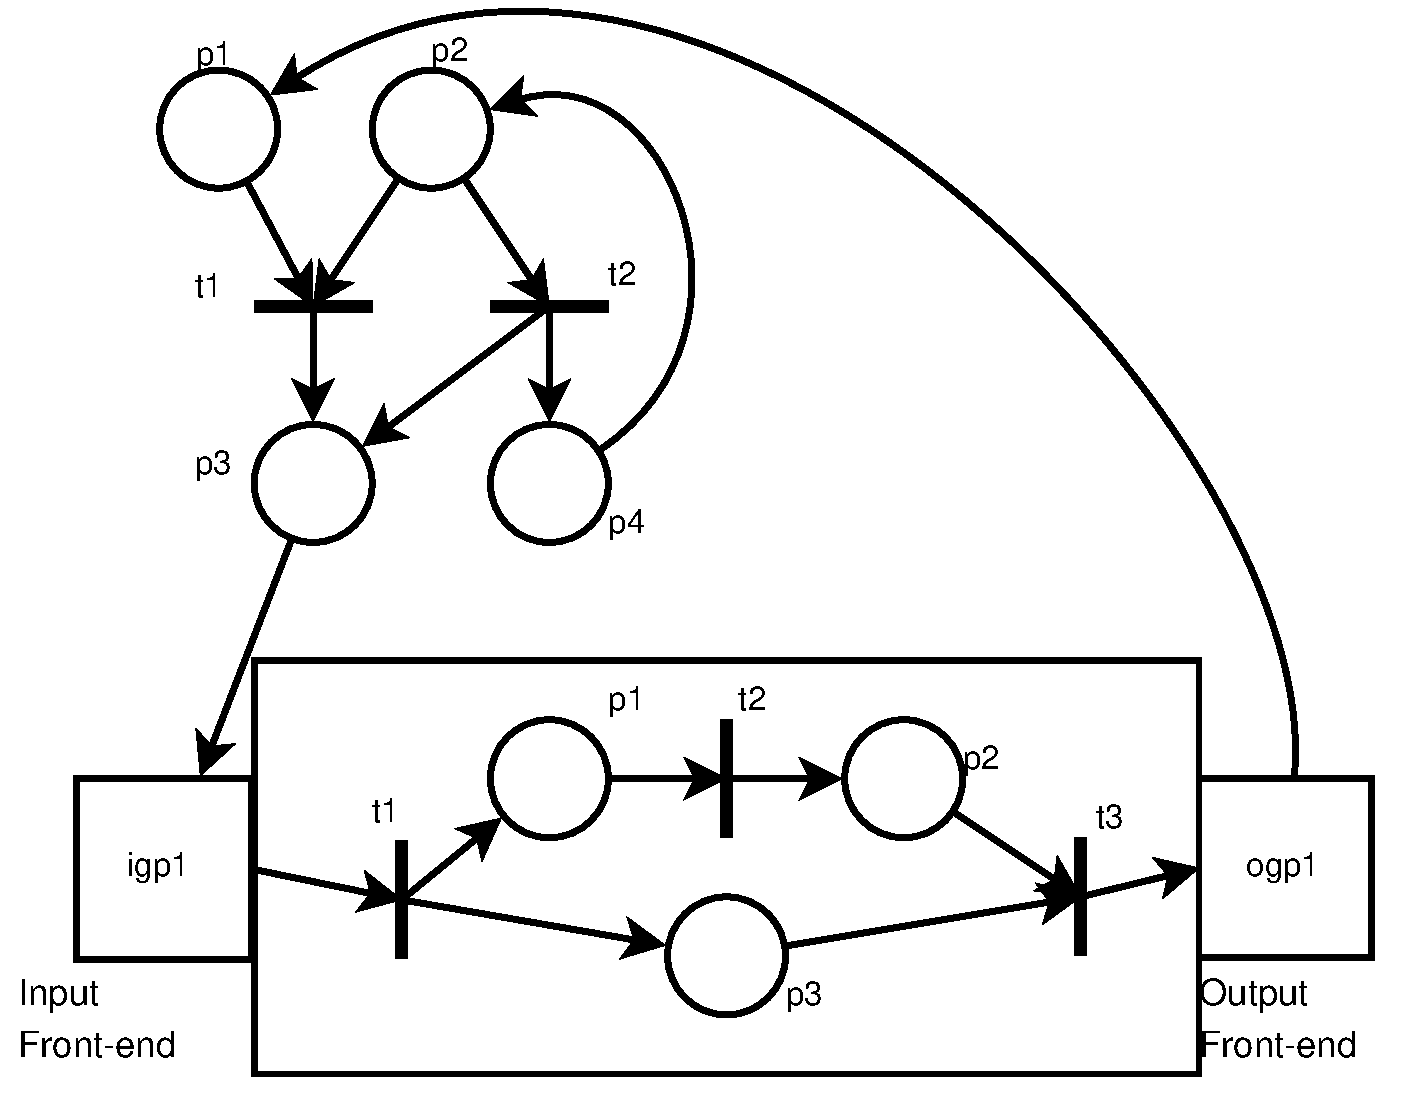
\includegraphics[width=0.4\textwidth]{Figures/RedAcoplableProveedor_1English.eps}\end{matrix}
 b) \ \ 
 \begin{matrix}  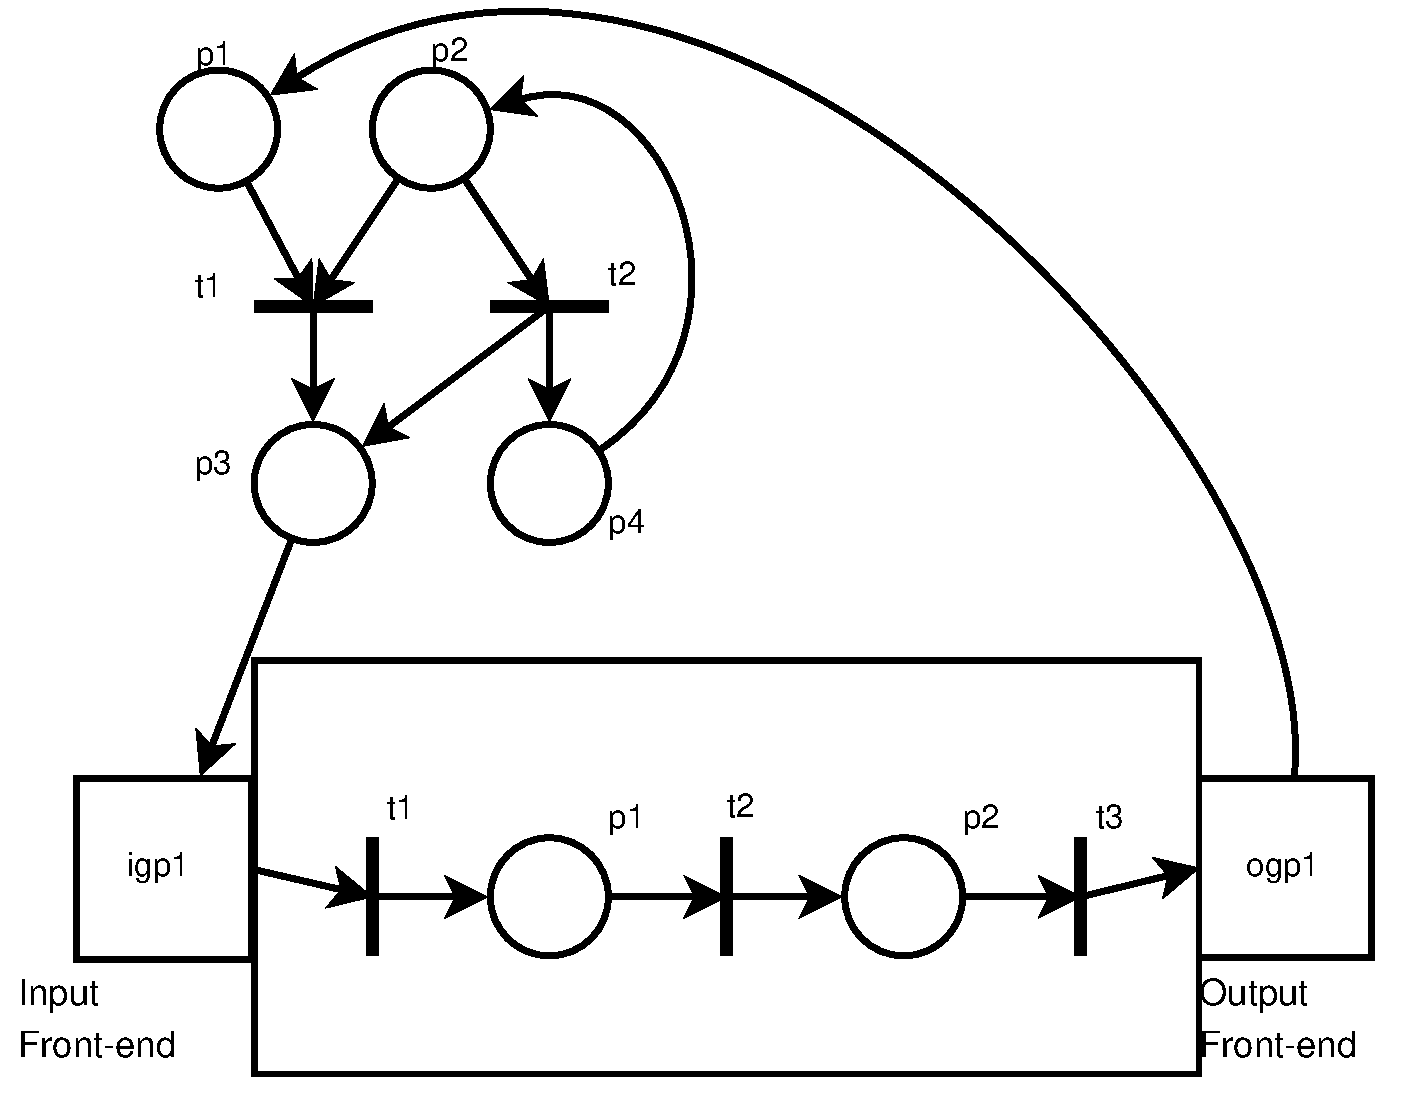
\includegraphics[width=0.4\textwidth]{Figures/RedAcoplableProveedor_2English.eps}\end{matrix}
\]
\rule{35em}{0.5pt}
\caption{Two different implementations of attachable nets}
\label{fig:redes_acoplables}
\end{figure*}
In this case, the behavior of the net will be the same, but does not have to be. That will decide who connects nets. For example, you could create a'' silly'' net that does nothing at first and replace it later by the real
one.
\end{example}

\section{Hiding vs. Reduction}

Both Silva works \cite{G-Silva1985,SM-Silva19931} as in the article by Xia \cite{R-Xia20111662} discusses possible Petri nets reductions for grouping and simplifying, under certain circumstances, places and / or transitions. These reductions can be structural (only dependent on the structure and initial marking of the net) or depending on the interpretation of the Petri net.

Should be clear that these reductions are not the same thing we are describing. We do not try to simplify the network together elements to have more or fewer places or transitions or to make it easier. What we want is to hide part of the network, regardless of how simple or complicated it is.

Here we have an example of what a reduction is.

\begin{example}[Reduction of an implicit place \cite{G-Silva1985}]
\label{ej:ocultacion_reduccion}
In a marked Petri net, an implicit place is one that meets the following:
\begin{shortenumerate}
 \item its marking can be calculated from other points marking
 \item never is the only place that prevents the enabling of its output transitions
\end{shortenumerate}
If we consider the following Petri net
\[
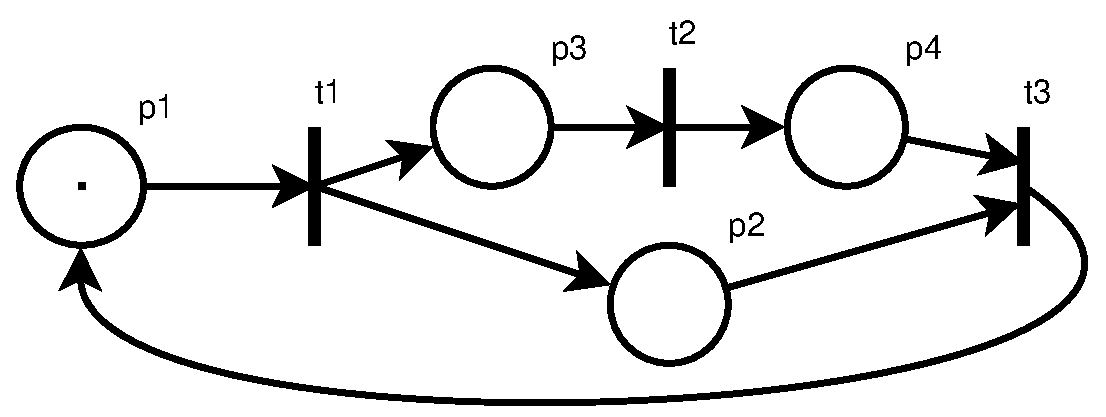
\includegraphics[width=0.5\textwidth]{Figures/OcultacionVsReduccion_1.eps}
\]
we can notice that $p_2$ is an implicit place because its marking can be
calculated as a function of $p_3$ y $p_4$:
\[
M(p_2) = M(p_3) + M(p_4)
\]
Moreover, by this same formula, it is clear that $ M (p_2) \geq M (P_4) $ (marking cannot be negative) so the only place that can prevent enabling of $ T_3 $ is $ P_4 $. Thus eliminating $ p_2$ does not alter the behavior of the network, which would be as follows:
\[
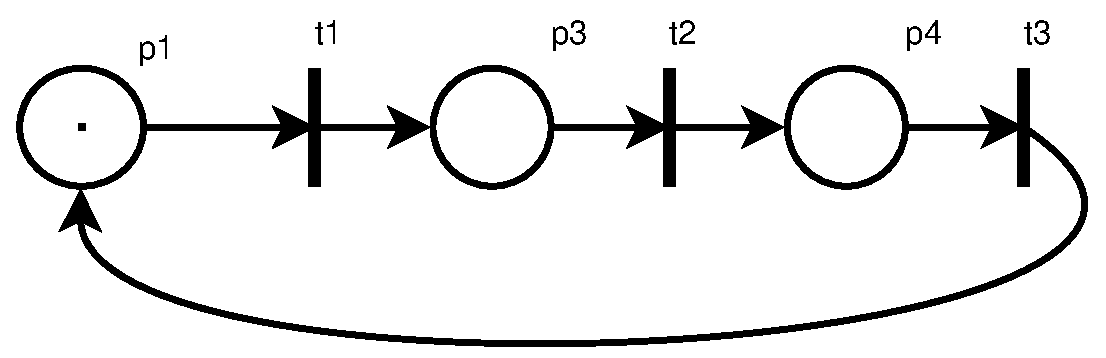
\includegraphics[width=0.5\textwidth]{Figures/OcultacionVsReduccion_2.eps}
\]
In this network elements have been removed, no hidden. This example helps us to see the difference between hiding and a reduction.
\end{example}  

\section{Conclusions}
As we have seen, any Petri net can be divided into any number of subnets, only limited by the number of places and transitions. Furthermore, each one of this Petri subnets has its own input and output front-ends in order to
connect with the rest of the Petri net.
Of course, the main application of this definitions in this thesis
is that the private information of this Petri net is stored in one or more
of these defined subnets.

 So I have reached the first milestone: Extend Petri Nets definition in order to define the public and the private information.  
 
% Chapter Template

\chapter{Petri net representation for subnets and hiding support. PNML} % Main chapter title

\label{Petri net representation for subnets and hiding support. PNML} % Change X to a consecutive number; for referencing this chapter elsewhere, use \ref{Chapter3}

\lhead{Chapter . \emph{Petri net representation for subnets and hiding support. PNML}} % Change X to a consecutive number; this is for the header on each page - perhaps a shortened title

%----------------------------------------------------------------------------------------
%       SECTION 1
%----------------------------------------------------------------------------------------
\section{Introduction}

Once explained how to split a net in several subnets, the next step is to define a way to hide one or more of those subnets.

 There is not literature about this
topic. Because of that I have to do a previous work about Petri net representation.
First of all  a way to represent subnet must be defined. Depending on the selected representation, the way to occult subnets may
be different or even impossible.

\section{Petri net representations}
There are four standard ways to represent Petri nets. Each one of them have their
properties, advantages and disadvantages. But I want to select one that I am able to represent any kind of Petri net, its subnets and allow to hide information without erasing it. 

\subsection{Graphic representation}

This is the clearest and extended way to represent Petri nets. It has a
very important advantage and it is that a picture is worth a thousand words.


Subnets can be defined simply drawing a vertical line. The right part is
one subnet and the left part is other subnet. Places and transitions
can be moved from one location to another depending on the subnet they are
situated. This is only an example. Other way would be to use colors for the
nodes (same color indicates same subnet) or use rectangles, etc.

\begin{example}[Graphic representation of a hidden subnet]
\label{ej:graphic_representation_hidden_subnet}
Let's take the following Petri net.


\[
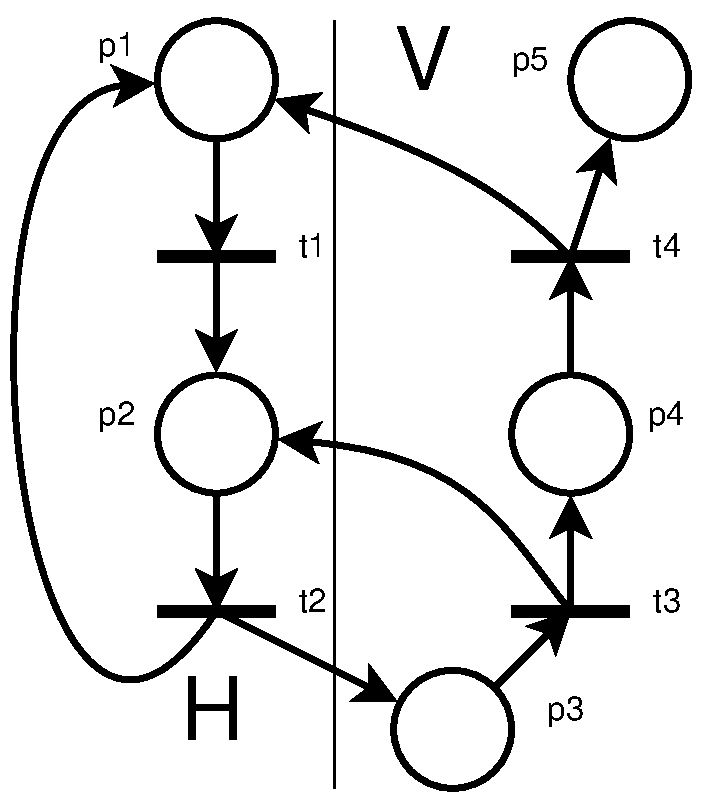
\includegraphics[width=0.3\textwidth]{Figures/EleccionSubredZonasInfluencia_2.eps}
\]



I want to occult the part marked with an H, so the result is this graphic

\[
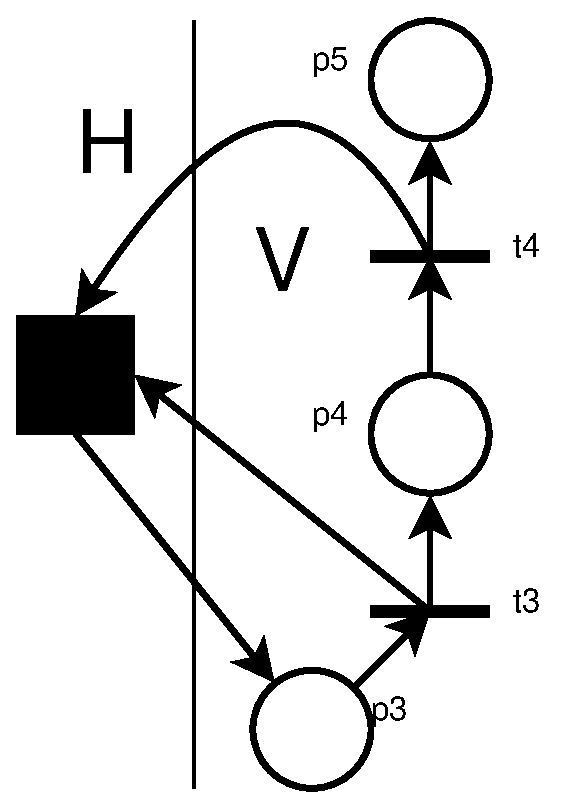
\includegraphics[width=0.25\textwidth]{Figures/OcultacionSubred_1.eps}
\]

And now, how can I maintain the H subnet information on the black box?
If I want to distribute  this Petri net I should send something more to that
people I want to access the hidden subnet. I have not found a way to embed
that information in the graphic so that some people can access it but other
people can't.
\end{example}

So this representation is useful in order to show at one sight the Petri
net structure, but I can't choose it  for my goals.
I have not been able to discover a way to show some people the hidden
information (the hidden subnet). However I will continue using it where a clear idea of the Petri structure
if necessary.

\subsection{Matrix representation}
This representation is very useful to study properties and evolution of a
Petri net, independently of its graphic representation.
As we have seen before (in chapter \ref{Chapter3}), we can reorder rows and columns and define subnets
in the matrix.
\begin{example}[Matrix representation of a hidden subnet]
\label{ej:matrix_representation_hidden_subnet}
This is the matrix representation of the Petri net in the previous example
\ref{ej:graphic_representation_hidden_subnet}.
\[
\kbordermatrix{
   & t_1 & t_2 & t_3 & t_4\\
p_1& -1 &  1  &  0  &  1 \\
p_2&  1 & -1  &  1  &  0 \\
p_3&  0 &  1  & -1  &  0 \\
p_4&  0 &  0  &  1  & -1 \\
p_5&  0 &  0  &  0  &  1 \\
}
\]

As we can see before,  If I occult the part marked with an H, so the result is:
\[
\kbordermatrix{
   & t_1 &  t_2 & \vline &t_3 & t_4\\
p_1& \rule{0.15in}{0.15in} & \rule{0.15in}{0.15in}    & \vline &  0  &  1 \\
p_2& \rule{0.15in}{0.15in} & \rule{0.15in}{0.15in}   & \vline &  1  &  0 \\
\hline
p_3&  0 &  1  & \vline & -1  &  0 \\
p_4&  0 &  0  & \vline &  1  & -1 \\
p_5&  0 &  0  & \vline &  0  &  1 \\
}
\]

or this other one, grouping the places and transitions of the hidden subnet as seen in chapter \ref{Chapter3}
\[
\kbordermatrix{
   &  _ & \vline &t_3 & t_4\\
p_2 & \rule{0.15in}{0.15in}   & \vline &  1  &  1 \\
\hline
p_3&  1  & \vline & -1  &  0 \\
p_4&  0  & \vline &  1  & -1 \\
p_5&  0  & \vline &  0  &  1 \\
}
\]


And now I have the same problems as in graphic mode: how can I keep  information
in the black box?
\end{example}

With this representation it is possible to study properties and it may be really important
as a complement to graphic mode. With both representations together, everyone has a clear idea of the Petri net structure and properties.  But I haven't
found a way to store information inside the black box. 

\subsection{Equation representation}
The third representation way for Petri nets is the equation representation.
Basically, transitions are selected and, for each one, the tokens of the places
connected to that transition are modified. This is very useful to compute
the evolution of a Petri net, choosing the transition fired.

However it is difficult to find a way for representing subnets with this
notation. And, of course, if a subnet cannot be represented, it cannot be
hidden. 

\begin{example}[Equation representation of a hidden subnet]
\label{ej:equation_representation_hidden_subnet}
Let's take again the Petri net from the previous examples \ref{ej:graphic_representation_hidden_subnet}.
This is It's equation representation:

\begin{scriptsize}
\begin{alltt}
if (p1>0) then
        p1 <- p1 - 1
        p2 <- p2 + 1
if (p2>0) then
        p2 <- p2 - 1
        p1 <- p1 + 1
        p3 <- p3 + 1
if (p3>0) then
        p3 <- p3 - 1
        p2 <- p2 + 1
        p4 <- p4 + 1
if (p4>0) then
        p4 <- p4 - 1
        p1 <- p1 + 1
        p5 <- p5 + 1
\end{alltt}
\end{scriptsize}

As we can see, we should hide several lines. In particular all that includes
places $p_1$ and $p_2$, resulting something like this (strikethrough text
would be part of the subnet):

\begin{scriptsize}
\begin{alltt}
\xout{if (p1>0) then}
        \xout{p1 <- p1 - 1}
        \xout{p2 <- p2 + 1}
\xout{if (p2>0) then}
        \xout{p2 <- p2 - 1}
        \xout{p1 <- p1 + 1}
        p3 <- p3 + 1
if (p3>0) then
        p3 <- p3 - 1
        \xout{p2 <- p2 + 1}
        p4 <- p4 + 1
if (p4>0) then
        p4 <- p4 - 1
        \xout{p1 <- p1 + 1}
        p5 <- p5 + 1
\end{alltt}
\end{scriptsize}

This is probably the strangest way to represent Petri nets and it is difficult
to define subnets over it.

\end{example}


I have tried to think about these ways of representation but, in my opinion, no one of them is suitable enough to represent subnets in a clear way than can be occulted. Because of that I have chosen the fourth representation, which is PNML, and that is explained in the next section. 

%----------------------------------------------------------------------------------------
%       SECTION 2
%----------------------------------------------------------------------------------------
\section{PNML. Petri Net Marked Language}

Originally, with basic Petri nets, the structure of a Petri net was fully provided.
The only thing that is not supported in comparison with graphic mode is the graphical appearance of Petri nets: the position of nodes and
transitions was not
important, but with the arrival of High level Petri nets and Petri nets design
software, is necessary to store this kind of information.

After several years of study, in 2004 the ISO/IEC 15909-1  \cite{PNML-iso/iec-15909-1} appeared to define conceptually and mathematically a xml representation
of Petri nets: PNML\cite{PNML-Hillah2006307}.  


So all the Petri nets that I am able to draw can be stored in PNML. Because
of that, it is one of the most supported formats in almost every program that
draw Petri nets. 

PNML \cite{PNML-pnml.org} is an implementation defined by the standard ISO/IEC 15909-2:2014 \cite{PNML-iso/iec-15909-2:2011}. The goal of this ISO standard is to define a transfer format of Place/Transition nets, High-level Petri nets and Symmetric nets. However, it is designed in
such way that it can be easily extended, so that other versions of Petri
nets can be supported later.
There is a way to define these extensions in a graphical way, using eclipse
as intermediate \cite{PNMLE-Kindler2011318,PNMLE-Hillah201246}, but this
is not the main goal of my work. My intention is to describe this extension
in a theoretical way. Once described, it could be implemented with that kind
of tools.

In this work, I am going to study only basic Petri nets, but
that concept and the method is easily exportable to other kind of nets, such as Symmetric nets and High Level Petri nets (that are representable in PNML
format too.)

\subsection{Scope}
The scope of this work in this section is basically bounded by the original
and basic Petri nets, that is:
\begin{itemize}
\item there are places, transitions and arcs between them
\item places can have tokens on them (but this does not have influence in
the hidding process)
\item transitions can be fired, but there is only one type of transition
(not messages, not time, etc.)
\end{itemize}

Furthermore, I am going to explain several concepts for a specific graphical
design of the Petri net (that will not influence the process either).

There are other options such as specific information for the design tool
that I am not going to discuss because the tools have no interest in this work 

\subsection{Description}
Petri Net Marked Language is an xml language created to represent Petri Nets. With this language we can take a Petri Net and store it into an xml file without loss of information.

One of the best properties of PNML is that, as it is an xml based schema,
it can be extended with more functionality extending the grammar.
Virtually, any extension over Petri nets can be translated into PNML in a logical and natural way.
Moreover, this extension is defined by Petri net type definition \cite{PNML-Billington2003483,PNML-iso/iec-15909-2:2011}.
 

In this case PNML hasn't got a way to represent subnets. There is something named \texttt{\textless page\textgreater}\ 
that is used to represent several nets in the same PNML file. But, by default,
a node inside a page cannot connect with a node of other page. So it cannot
be used as "subnets". So I am going to extend the language in order to get several goals:
\begin{enumerate}
\item Represent subnets of a Petri Net.
\item Include input and output interfaces for every subnet.
\end{itemize}

As we can think, definition of several subnets of a Petri net is possible
and the connection over them are always through their respective interfaces.

\subsection{PNML grammar}

As PNML is an xml based language it has to be described by an schema that define the creation rules of the PNML representation of a Petri net.

The grammar is defined since 2009 and updated until
2012, which is the most recent revision.
I am not going to do and extensive explanation of all the possibilities
of the grammar, but the most important. As we can see later, anything we think is useful can be added to the process with little effort.
So I am going to study only the most basic elements of a Petri net. The rest of the element can be attached later with facility. 

\subsubsection{PNML basics}

In this section I am going to explain several characteristics of PNML files.
With these explanations it is going to be easier the understanding of PNML
structure.

First of all, as PNML files are xml files, there several things to know:

\begin{enumerate}
\item 
  A xml file normally starts with a line defining some characteristics of
  the file, like the version and the encoding type. It has an aspect like
  this\footnote{For clarity, in the following examples, this line can be deleted.}: 

\begin{lstlisting}
<?xml version="1.0" encoding="utf-8"?>
\end{lstlisting}
  
 
\item
  A root node must exist.
  In this case, the root node is \texttt{\textless pnml\textgreater}.
  So every PNML files has to start with the tag \texttt{\textless pnml\textgreater}\   and end with the tag \texttt{\textless/pnml\textgreater}.
Below this tag, there is a new tag \texttt{\textless net\textgreater}\ that can contain
  \begin{itemize}
  \item Type: the type of the Petri net as an attribute. In this case, as
    I  am going to study only Place/Transition nets, it will  be \texttt{ptnet}
  \item Name of the net: New tag \texttt{\textless name\textgreater\textless text\textgreater...\textless/text\textgreater\textless/name\textgreater}
  \item Pages: one page is an invention to store several Petri nets inside
  an unique PNML file, but usually there is only one page for file. It is
  nested inside a \texttt{\textless page\textgreater}\ tag.
  \end{itemize}
  \item
  Each element in PNML has to have a unique id inside the net to be identified
unambiguously. So there cannot
  be two elements with the same id.
\end{enumerate}

 

With this three observations, we can have an idea about how a PNML file
is structured:  

 
\begin{lstlisting}[label=pnml_net_page,caption=Example of general PNML file]
<?xml version="1.0" encoding="utf-8"?>
<pnml>
  <net id="myNet" type="http://www.pnml.org/version-2009/grammar/ptnet">
    <name>
      <text> My new net </text>
    </name>
    <page id="page1">
      .......
    </page>
  </net>
</pnml>
\end{lstlisting}

Once this structure is defined, I am going to explain the next stage, that
is the most important one in this work. 

\subsubsection{Places, transitions and arcs in PNML}

As Petri nets has three main elements, places, transitions
and arcs, and PNML has them too. These three elements have several things in common in an PNML file:
\begin{itemize}
  \item They are all nested in a page tag


  \item Places and transitions (not arcs) can contain a tag \texttt{\textless name\textgreater}\ with its name. This tag has been defined before for the name of the net. It
can store information about the text of the name and the graphical position
of this label in this way:
\begin{lstlisting}
<name>
  <text> Element Name </text>
  <graphics>
    <offset x="22" y="-10"/>
  </graphics>
</name>
\end{lstlisting}
   \item They can contain a tag \texttt{\textless graphics\textgreater}\ with information about its position and dimension:
\begin{lstlisting}
<graphics>
  <position x="100" y="200"/>
  <dimension x="40" y="40"/>
</graphics>
\end{lstlisting}
\end{itemize}


These are the common properties of places, transitions and arcs. Now let's
go on the particular characteristics of each one of them.

Places are represented with the tag \texttt{\textless place\textgreater}\ and the can have a marking with the label \texttt{\textless initialMarking\textgreater}.
Here we have an example of a place with two tokens in PNML: 

\begin{lstlisting}[label=pmnl_place,caption=PNML representation
for places]
<place id="p1">
  <name>
    <text> Place number one </text>
    <graphics>
      <offset x="130" y="130"/>
    </graphics>
  </name>
  <graphics>
    <position x="130" y="90"/>
    <dimension x="40" y="40"/>
  </graphics>
  <initialMarking>
    <text> 2 </text>
  </initialMarking>
</place>
\end{lstlisting}

Transitions are represented with the tag \texttt{\textless transition\textgreater}.
This is an example of a transition in PNML: 

\begin{lstlisting}[label=pmnl_transition,caption=PNML representation
for transitions]
<transition id="t1">
  <name>
    <text> Transition number one </text>
    <graphics>
      <offset x="270" y="140"/>
    </graphics>
  </name>
  <graphics>
    <position x="270" y="100"/>
    <dimension x="40" y="40"/>
  </graphics>
</transition>
\end{lstlisting}

Arcs are represented with the tag \texttt{\textless arc\textgreater}. Arc
have to have a source and a target, which are defined by the attributes \texttt{source} and \texttt{target} that have to point to a transition and a place, identified
by their id. Furthermore, the arc weight can be fixed by the \textless inscription\textgreater\
 tag.
If the weight is one, the tag inscription is not necessary because this is
the default value. This is an example of the arc with weight 3 that connects the place and the
transition of the previous examples in PNML: 

\begin{lstlisting}[label=pmnl_arc,caption=PNML representation
for arcs]
<arc id="a1" source="p1" target="t1">
  <inscription> 3 </inscription>
</arc>
\end{lstlisting}

\newpage
If we take the last examples all together, we can represent the following Petri net:

\[
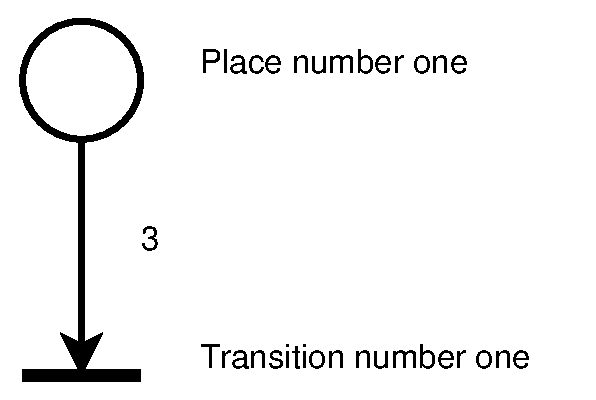
\includegraphics[width=0.25\textwidth]{Figures/PNML-RdPBasicaCompleta.eps}
\]

\begin{lstlisting}[label=pmnl_complete_representation,caption=Complete PNML representation
for a basic Petri net]
<?xml version="1.0" encoding="utf-8"?>
<pnml>
  <net id="myNet" type="http://www.pnml.org/version-2009/grammar/ptnet">
    <name>
      <text> My new net </text>
    </name>
    <page id="page1">
      <place id="p1">
        <name>
          <text> Place number one </text>
          <graphics>
            <offset x="130" y="130"/>
          </graphics>
        </name>
        <graphics>
          <position x="130" y="90"/>
          <dimension x="40" y="40"/>
        </graphics>
        <initialMarking>
          <text> 2 </text>
        </initialMarking>
      </place>
      <transition id="t1">
        <name>
          <text> Transition number one </text>
          <graphics>
            <offset x="270" y="140"/>
          </graphics>
        </name>
        <graphics>
          <position x="270" y="100"/>
          <dimension x="40" y="40"/>
        </graphics>
      </transition>
      <arc id="a1" source="p1" target="t1">
        <inscription> 3 </inscription>
      </arc>
    </page>
  </net>
</pnml>
\end{lstlisting}

For clarity, I am going to obviate several options. I am not going to put the graphic information and the names, but the id. So this last example is as follows:

\[
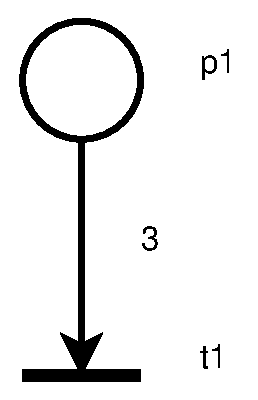
\includegraphics[width=0.1\textwidth]{Figures/PNML-RdPBasica.eps}
\]

\begin{lstlisting}[label=pmnl_basic_representation,caption=Basic PNML representation
for a basic Petri net]
<?xml version="1.0" encoding="utf-8"?>
<pnml>
  <net id="myNet" type="http://www.pnml.org/version-2009/grammar/ptnet">
    <page id="page1">
      <place id="p1">
        <initialMarking>
          <text> 2 </text>
        </initialMarking>
      </place>
      <transition id="t1"/>
      <arc id="a1" source="p1" target="t1">
        <inscription> 3 </inscription>
      </arc>
    </page>
  </net>
</pnml>
\end{lstlisting}


I think that this last listing is clear enough to understand the rest of
the process. But not only that. For even more clarity, the tags \texttt{\textless ?xml\textgreater}, \texttt{\textless pnml\textgreater}, \texttt{\textless net\textgreater}\ and \texttt{\textless page\textgreater} are going to be obviated
too. So in many of the later examples they will not be present. Applying
this criterium, the listing \ref{pmnl_basic_representation} change to:

\begin{lstlisting}[label=pmnl_simplified_representation,caption=Simplified PNML representation
for a basic Petri net]
<place id="p1">
  <initialMarking>
    <text> 2 </text>
 </initialMarking>
</place>
<transition id="t1"/>
<arc id="a1" source="p1" target="t1">
  <inscription> 3 </inscription>
</arc>
\end{lstlisting}








\subsection{PNML examples}

In this section I will present several examples of  Petri nets represented with PNML. This examples are extracted directly form \url{www.pnml.org}.
These examples will be processed later in order to hide parts of them.

As first example, we have the Dining Philosophers...

//TODO terminar 

\subsection{PNML extension for representing subnets}


 In this section I am going to define new tags and structures in PNML. At this point, I have developed all the necessary to extend PNML in order
to represent subnets.

Let's take the following simple Petri net that will serve us to explain
the method to achieve a subnet representation and the PNML extension associated
to it:

\[
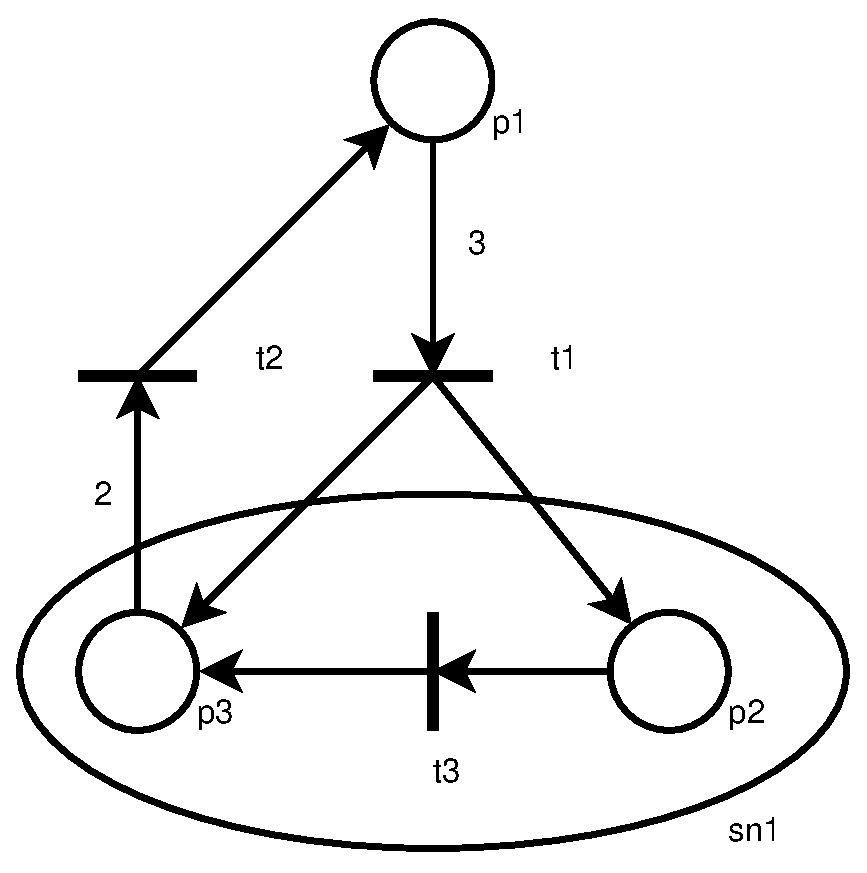
\includegraphics[width=0.40\textwidth]{Figures/PNML-RdPSubred.eps}
\]

The PNML code for this net is:

\begin{lstlisting}
<place id="p1"/>
<place id="p2"/>
<place id="p3"/>
<transition id="t1"/>
<transition id="t2"/>
<transition id="t3"/>
<arc id="a1" source="p1" target="t1">
  <inscription>
    <text> 3 </text>
  </inscription>
</arc>
<arc id="a2" source="t1" target="p2"/>
<arc id="a3" source="t1" target="p3"/>
<arc id="a4" source="p3" target="t2">
  <inscription>
    <text>2</text>
  </inscription>
</arc>
<arc id="a5" source="t3" target="p3"/>
<arc id="a6" source="p2" target="t3"/>
<arc id="a7" source="t2" target="p1"/>
\end{lstlisting}

I want the ellipse region to be a subnet, so I have to specify a subnet with the elements inside the ellipse.



The first step is to define a new tag \texttt{\textless subnet\textgreater}. This tag will have an id, as the rest of PNML elements. And now we proceed
in this way:

\begin{enumerate}
\item The places and transitions inside the subnet are moved into the \textless subnet\textgreater\ tag
\item The arcs joining subnet elements will be included inside the tag
\item The arcs entering or leaving the subnet will be copied inside the tag.
This mean that there are arcs duplicated inside and outside the tag
\end{enumerate}


If we apply these rules to the example:

\begin{enumerate}
\item $p2$, $p3$ and $t3$ are moved into the tag \texttt{\textless subnet\textgreater}
\item $a5$ and $a6$ are put inside the tag
\item $a2$, $a3$ and $a4$ are copied inside the tag
\end{enumerate}

and we have this other PNML extended code: 

\begin{lstlisting}
<subnet id="sn1">
  <place id="p2"/>
  <place id="p3"/>
  <transition id="t3"/>
  <arc id="a2" source="t1" target="p2"/>
  <arc id="a3" source="t1" target="p3"/>
  <arc id="a4" source="p3" target="t2">
    <inscription>
      <text> 2 </text>
    </inscription>
  </arc>
  <arc id="a5" source="t3" target="p3"/>
  <arc id="a6" source="p2" target="t3"/>
</subnet>
<place id="p1"/>
<transition id="t1"/>
<transition id="t2"/>
<arc id="a1" source="p1" target="t1">
  <inscription>
    <text> 3 </text>
  </inscription>
</arc>
<arc id="a2" source="t1" target="p2"/>
<arc id="a3" source="t1" target="p3"/>
<arc id="a4" source="p3" target="t2">
  <inscription>
    <text> 2 </text>
  </inscription>
</arc>
<arc id="a7" source="t2" target="p1"/>
\end{lstlisting}

Now this is one of the most important moment in this work: I will separate the inside
and the outside of the subnet completely. Taking advantage of the process described in chapter \ref{Chapter3}, I have to extract the front-end from this subnet.

In this case I have two igp (input gate to a place) and an ogt (output gate to a transition). This graphic illustrates the interface associated:

\[
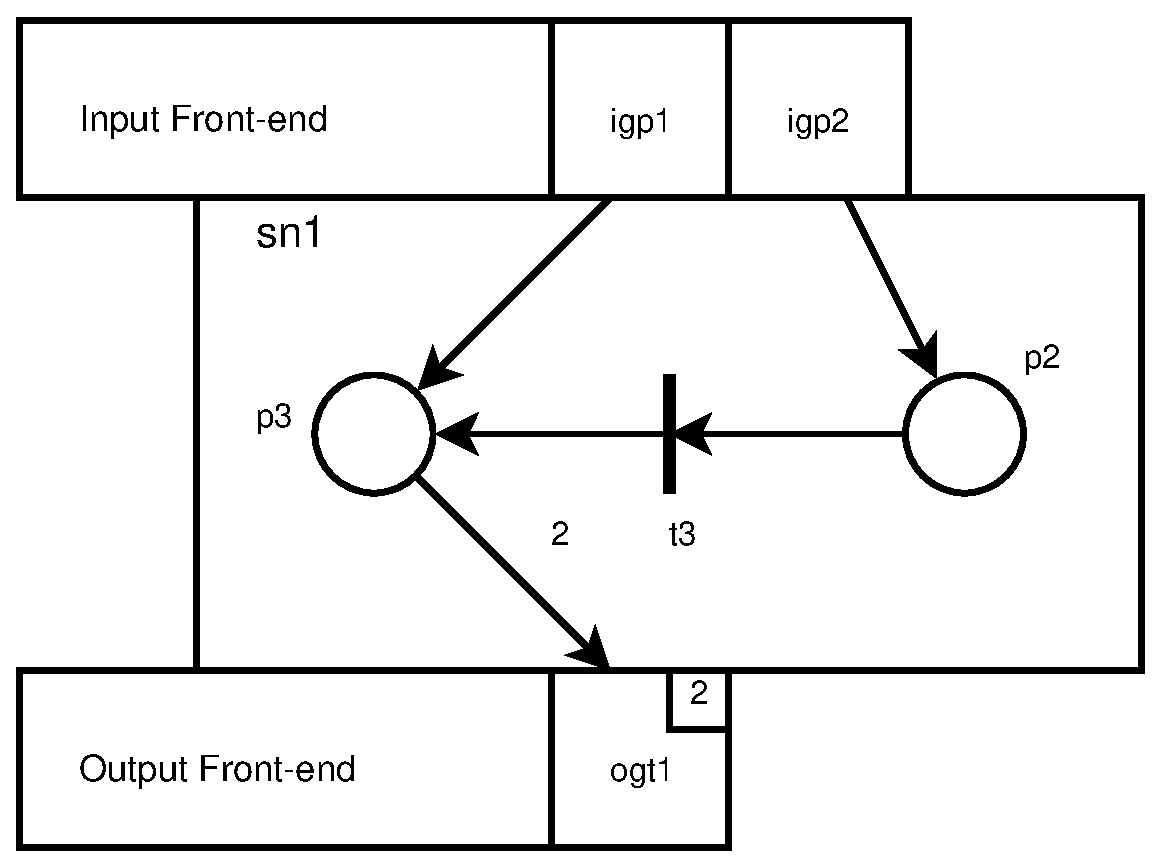
\includegraphics[width=0.60\textwidth]{Figures/PNML-InterfazSubredEjemplo1.eps}
\]

And this is the complete net including the subnet and its front-end

\[
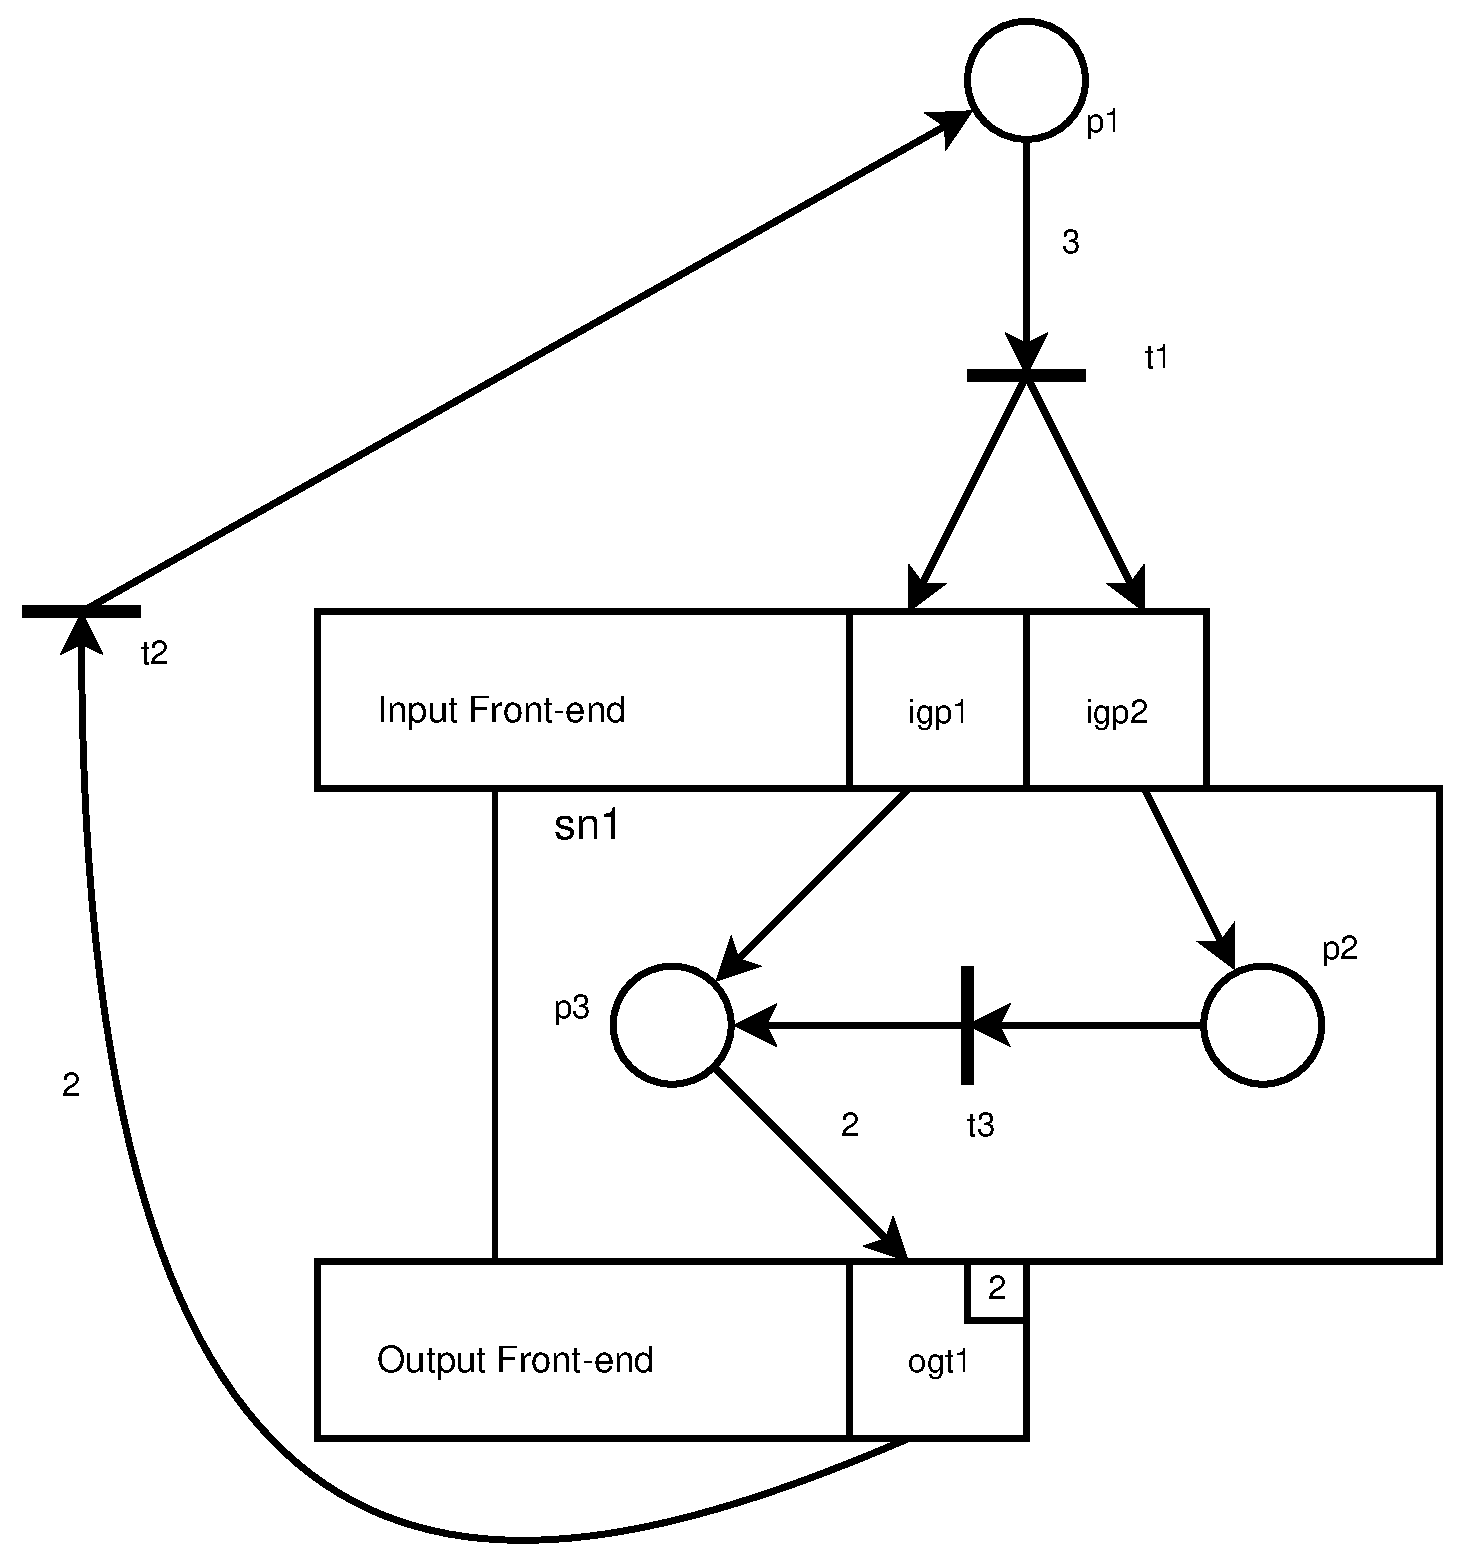
\includegraphics[width=0.60\textwidth]{Figures/PNML-SubredEjemplo1.eps}
\]
 
And now that I have the graphic, how can I represent it in PNML? To answer
this question I will define four new tags: \texttt{\textless interface\textgreater},
\texttt{\textless gate\textgreater}, \textless inscription\textgreater\ and \texttt{\textless content\textgreater}. Let's explain them.

As its name says, \texttt{\textless interface\textgreater}\ is
the tag name for encapsulate the front-end. This tag has no attributes (only
the id, of course)
but
it has embedded the gates inside of it. This gates are represented by \texttt{\textless gate\textgreater}. This tag has two new attributes: \texttt{action} and \texttt{type}.
These two attributes have information about the gates. The attribute \texttt{action}
can take two different values: \texttt{input} and \texttt{output}. It indicates
whether the gate is an input gate or an output gate. The other attribute,
\texttt{type}, can take other two values: \texttt{place} and \texttt{transition}.
As arcs have weight, gates have it too. For being in accordance, I define
the tag \texttt{\textless inscription\textgreater}\ embedded in the tag \texttt{\textless gate\textgreater}. It has the weight of the arc associated.\ 

There is one other tag \texttt{\textless content\textgreater}\ that
probably at this moment seems useless, but it is necessary for the rest of the process, as we will see in the next chapter. So I am going to introduce it now. This tag is used to encapsulate the rest of the subnet outside the interface. That is, \texttt{\textless subnet\textgreater}\ has two children:
\texttt{\textless interface\textgreater}\ and \texttt{\textless content\textgreater},
that have the input/output gates and the rest of the elements, respectively.

Applying this definition to the example, we will have this code

\begin{lstlisting}
<subnet id="sn1">
  <interface id="sn1-interface">
    <gate id="igp1" action="input" type="place"/>
    <gate id="igp2" action="input" type="place"/>
    <gate id="ogt1" action="output" type="transition">
      <inscription>
        <text> 2 </text>
      </inscription>
    </gate>
  </interface>
  <content id="sn1-content">
    <place id="p2"/>
    <place id="p3"/>
    <transition id="t3"/>
    <arc id="a2" source="t1" target="p2"/>
    <arc id="a3" source="t1" target="p3"/>
    <arc id="a4" source="p3" target="t2">
      <inscription>
        <text> 2 </text>
      </inscription>
    </arc>
    <arc id="a5" source="t3" target="p3"/>
    <arc id="a6" source="p2" target="t3"/>
  </content>
</subnet>
<place id="p1"/>
<transition id="t1"/>
<transition id="t2"/>
<arc id="a1" source="p1" target="t1">
  <inscription>
    <text> 3 </text>
  </inscription>
</arc>
<arc id="a2" source="t1" target="p2"/>
<arc id="a3" source="t1" target="p3"/>
<arc id="a4" source="p3" target="t2">
  <inscription>
    <text> 2 </text>
  </inscription>
</arc>
<arc id="a7" source="t2" target="p1"/>
\end{lstlisting}

At this moment I have to do only one thing more. The last step is to modify
the arcs that are repeated inside and outside the net changing their source or target, depending on where is it:

\begin{itemize}
\item If the arc is \textbf{entering} the subnet
  \begin{itemize}
  \item For the \texttt{\textless arc\textgreater} tag inside the tag \texttt{\textless subnet\textgreater}, the \textbf{source} attribute of the arc is changed by the \textbf{input} gate associated
  \item For the \texttt{\textless arc\textgreater} tag outside the tag \texttt{\textless subnet\textgreater}, the \textbf{target} attribute of the arc is changed by the \textbf{output} gate associated
  \end{itemize}
\item If the arc is \textbf{leaving} the subnet
  \begin{itemize}
  \item For the \texttt{\textless arc\textgreater} tag inside the tag \texttt{\textless subnet\textgreater}, the \textbf{target} attribute of the arc is changed by the \textbf{input} gate associated
  \item For the \texttt{\textless arc\textgreater} tag outside the tag \texttt{\textless subnet\textgreater}, the \textbf{source} attribute of the arc is changed by the \textbf{output} gate associated
  \end{itemize}
\end{itemize}

Applying again this rule to the example we have the definitive code for this
Petri net:

\begin{lstlisting}
<subnet id="sn1">
  <interface id="sn1-interface">
    <gate id="igp1" action="input" type="place"/>
    <gate id="igp2" action="input" type="place"/>
    <gate id="ogt1" action="output" type="transition">
      <inscription>
        <text> 2 </text>
      </inscription>
    </gate>
  </interface>
  <content id="sn1-content">
    <place id="p2"/>
    <place id="p3"/>
    <transition id="t3"/>
    <arc id="a2" source="igp2" target="p2"/>
    <arc id="a3" source="igp1" target="p3"/>
    <arc id="a4" source="p3" target="ogt1">
      <inscription>
        <text> 2 </text>
      </inscription>
    </arc>
    <arc id="a5" source="t3" target="p3"/>
    <arc id="a6" source="p2" target="t3"/>
  </content>
</subnet>
<place id="p1"/>
<transition id="t1"/>
<transition id="t2"/>
<arc id="a1" source="p1" target="t1">
  <inscription>
    <text> 3 </text>
  </inscription>
</arc>
<arc id="a2" source="t1" target="igp2"/>
<arc id="a3" source="t1" target="igp1"/>
<arc id="a4" source="ogt1" target="t2">
  <inscription>
    <text> 2 </text>
  </inscription>
</arc>
<arc id="a7" source="t2" target="p1"/>
\end{lstlisting}

Once this is done, the only way to enter or leave the subnet is crossing
the front-end. 







\section{Conclusions}



% Chapter Template

\chapter{XMLEncryption} % Main chapter title

\label{Chapter: XMLEncryption} % Change X to a consecutive number; for referencing this chapter elsewhere, use \ref{ChapterX}

\lhead{Chapter 5. \emph{XMLEncryption}} % Change X to a consecutive number; this is for the header on each page - perhaps a shortened title

%----------------------------------------------------------------------------------------
%       SECTION 1
%----------------------------------------------------------------------------------------
\section{Introduction}

There can be several reasons for hiding information of a Petri net. For example:

\begin{itemize}
\item One subnet is a secret process that I want to hide from indiscrete
eyes
\item I have a main process that communicates with other processes. These
processes are susceptible to be changed and the only information I need is
the interface, so they can be easily replaced by other implementations.
\end{itemize}
   But this information should be accessible to authorized
people without necessity of supplying any other kind of data.
So the whole information may be stored in the same file.


I think that the best way to reach this goal is using standard and proved
technologies. In this case, the selected technology is XMLEncryption.\cite{XMLENC-w3.org/xmlenc-core1}


\section{XMLEncryption revision}
XMLEncription is a World Wide Web Consortium (W3C)
Recommendation form  encrypt xml or non xml content. It is an xml file ciphering standard. Both symmetric and asymmetric ciphering can be used, but in this case, symmetric is preferred.
The main idea of this encryption is to replace the xml element or elements
we want to be ciphered by other xml code that contains the ciphered data, in addition to information of the algorithms used for the encryption process. When a non xml file in ciphered, the only option is to encrypt it completely. But,  when it is applied to xml content, this technology allows us to define concrete fragments of the document we want to hide. Moreover, the xml document can be transformed before applying the encryption, for example, in order to format the normalize the xml content.
In this work, the pieces of xml content susceptible to be ciphered are, obviously,
the subnets represented in PNML format. 

Regardless of the data source (xml or non xml) the result is always a xml element. Normal is that this xml encrypted chunk have the whole necessary information to be decrypted. Among that information we can find:

\begin{itemize}
\item Ciphering algorithm: it is the name of chosen method for ciphering
the data. It can be not included. In this case, both ciphering and deciphering agents have to know which is the exact this algorithm.
\item The ciphered data: obviously this parts is mandatory and has always
to be present.
\item Name of the chosen key: it is optional. It is used when a set of keys is known by both ciphering an deciphering agents.
\item Key: it is optional. In this case there is a symmetric key in order
to encrypt the data and an additional pair of keys: one (known by the cipher
agent) to encrypt the symmetric key and the other (known by the decipher agent) to decrypt it. 
\end{itemize} 

This section does not want to be an extensive explanation about XMLEncryption
but a general idea about its functionality. So I am not going to deepen the
whole characteristics of XMLEncryption. The final decision about which options
use is responsibility of those people that want to apply this work, basing their decision on the requirements of their own Petri net. 
 
Once this is said, here we have a basic example of XMLEncryption. Let's take this original xml document:

\begin{lstlisting}[label=xmlenc_example_1_1,caption=Clear xml content]
<?xml version='1.0'?>
<PaymentInfo xmlns='http://example.org/paymentv2'>
  <Name>John Smith</Name>
  <CreditCard Limit='5,000' Currency='USD'>
    <Number>4019 2445 0277 5567</Number>
    <Issuer>Example Bank</Issuer>
    <Expiration>04/02</Expiration>
  </CreditCard>
</PaymentInfo>
\end{lstlisting}

In this example, we want to hide the credit card number \texttt{\textless Number\textgreater}. Several options are going to be applied: with and without
the ciphering information


First of all let's see which will be the aspect of the ciphered content without
information about ciphering, only replacing the clear data by the encrypted
data:
we have not information about  the key or the ciphering algorithm. This
is the xml ciphered code:
\begin{lstlisting}[label=xmlenc_example_1_2,caption=Ciphered xml content
without ciphering information]
<?xml version='1.0'?>
<PaymentInfo xmlns='http://example.org/paymentv2'>
  <Name>John Smith</Name>
  <CreditCard Limit='5,000' Currency='USD'>
    <Number>
      <xenc:EncryptedData xmlns='http://www.w3.org/2001/04/xmlenc#'
          Type='http://www.w3.org/2001/04/xmlenc#Content'>
        <xenc:CipherData>
          <xenc:CipherValue>A23B45C56</CipherValue>
        </CipherData>
      </EncryptedData>
    </Number>
    <Issuer>Example Bank</Issuer>
    <Expiration>04/02</Expiration>
  </CreditCard>
</PaymentInfo>
\end{lstlisting}

As we can see, the credit card number has been replaced by a new 
tag \texttt{\textless EncryptedData\textgreater} that contains the ciphered credit card number.

\note{A new namespace \texttt{xenc} appear  that is the standard namespace
for XMLEncryption. However, in futher examples this namespace can be delete
for clarity and for space problems without loss of generality.}

And now let's see how does this same example with information about the algorithm:

\begin{lstlisting}[label=xmlenc_example_1_3,caption=Ciphered xml content
with algorithm information]
<?xml version='1.0'?>
<PaymentInfo xmlns='http://example.org/paymentv2'>
  <Name>John Smith</Name>
  <CreditCard Limit='5,000' Currency='USD'>
    <Number>
      <xenc:EncryptedData xmlns='http://www.w3.org/2001/04/xmlenc#'
          Type='http://www.w3.org/2001/04/xmlenc#Content'>
        <xenc:EncryptionMethod  
            Algorithm="http://www.w3.org/2001/04/xmlenc#aes128-cbc"  
            xmlns:xenc="http://www.w3.org/2001/04/xmlenc#" />  
        <xenc:CipherData>
          <xenc:CipherValue>A23B45C56</CipherValue>
        </CipherData>
      </EncryptedData>
    </Number>
    <Issuer>Example Bank</Issuer>
    <Expiration>04/02</Expiration>
  </CreditCard>
</PaymentInfo>
\end{lstlisting}

As we can see, a new tag \texttt{\textless EncryptedMethod\textgreater}\ has
appeared
inside the \texttt{\textless EncryptedData\textgreater} tag with the algorithm used to cipher. In this case
is \texttt{aes128-cbc}. 

There is other method of Encryption that cipher the tag too. In this case,
we would have the next code:

\begin{lstlisting}[label=xmlenc_example_1_4,caption=Ciphered xml content
including the tag itself]
<?xml version='1.0'?>
<PaymentInfo xmlns='http://example.org/paymentv2'>
  <Name>John Smith</Name>
  <CreditCard Limit='5,000' Currency='USD'>
    <xenc:EncryptedData xmlns='http://www.w3.org/2001/04/xmlenc#'
        Type='http://www.w3.org/2001/04/xmlenc#Element'>
      <xenc:EncryptionMethod  
          Algorithm="http://www.w3.org/2001/04/xmlenc#aes128-cbc"  
          xmlns:xenc="http://www.w3.org/2001/04/xmlenc#" />  
      <xenc:CipherData>
        <xenc:CipherValue>A223B3B493G5C569M</CipherValue>
      </CipherData>
    </EncryptedData>
    <Issuer>Example Bank</Issuer>
    <Expiration>04/02</Expiration>
  </CreditCard>
</PaymentInfo>
\end{lstlisting}

As we can see, the tag \texttt{\textless Number\textgreater} 
has disappeared and it has been included into the \texttt{\textless CipherValue\textgreater}
of the \texttt{\textless CipherData\textgreater}.

 

This is a little approach to XMLEncryption functionality, but enough for
understanding the next section.


\section{XMLEncryption and Petri nets}

Once described XMLEncryption it is time to apply it in order to hide part
of a Petri net. Remembering the chapter \ref{Chapter: Petri net representation for subnets and hiding support. PNML}, we have one Petri net with or more subnets represented in a PNML file. These subnets are represented by a \texttt{\textless subnet\textgreater}\ tag that contains \texttt{\textless interface\textgreater}\ and
\texttt{\textless content\textgreater}. This last tag the
xml content that is going to be ciphered. Obviously, if we encrypt the interface
we will have no way to connect the subnet with the rest of the net.

Let's take back the example used to explain the process of subnetting in
the figure \ref{fig:PNML_SubredEjemplo1}...

\[
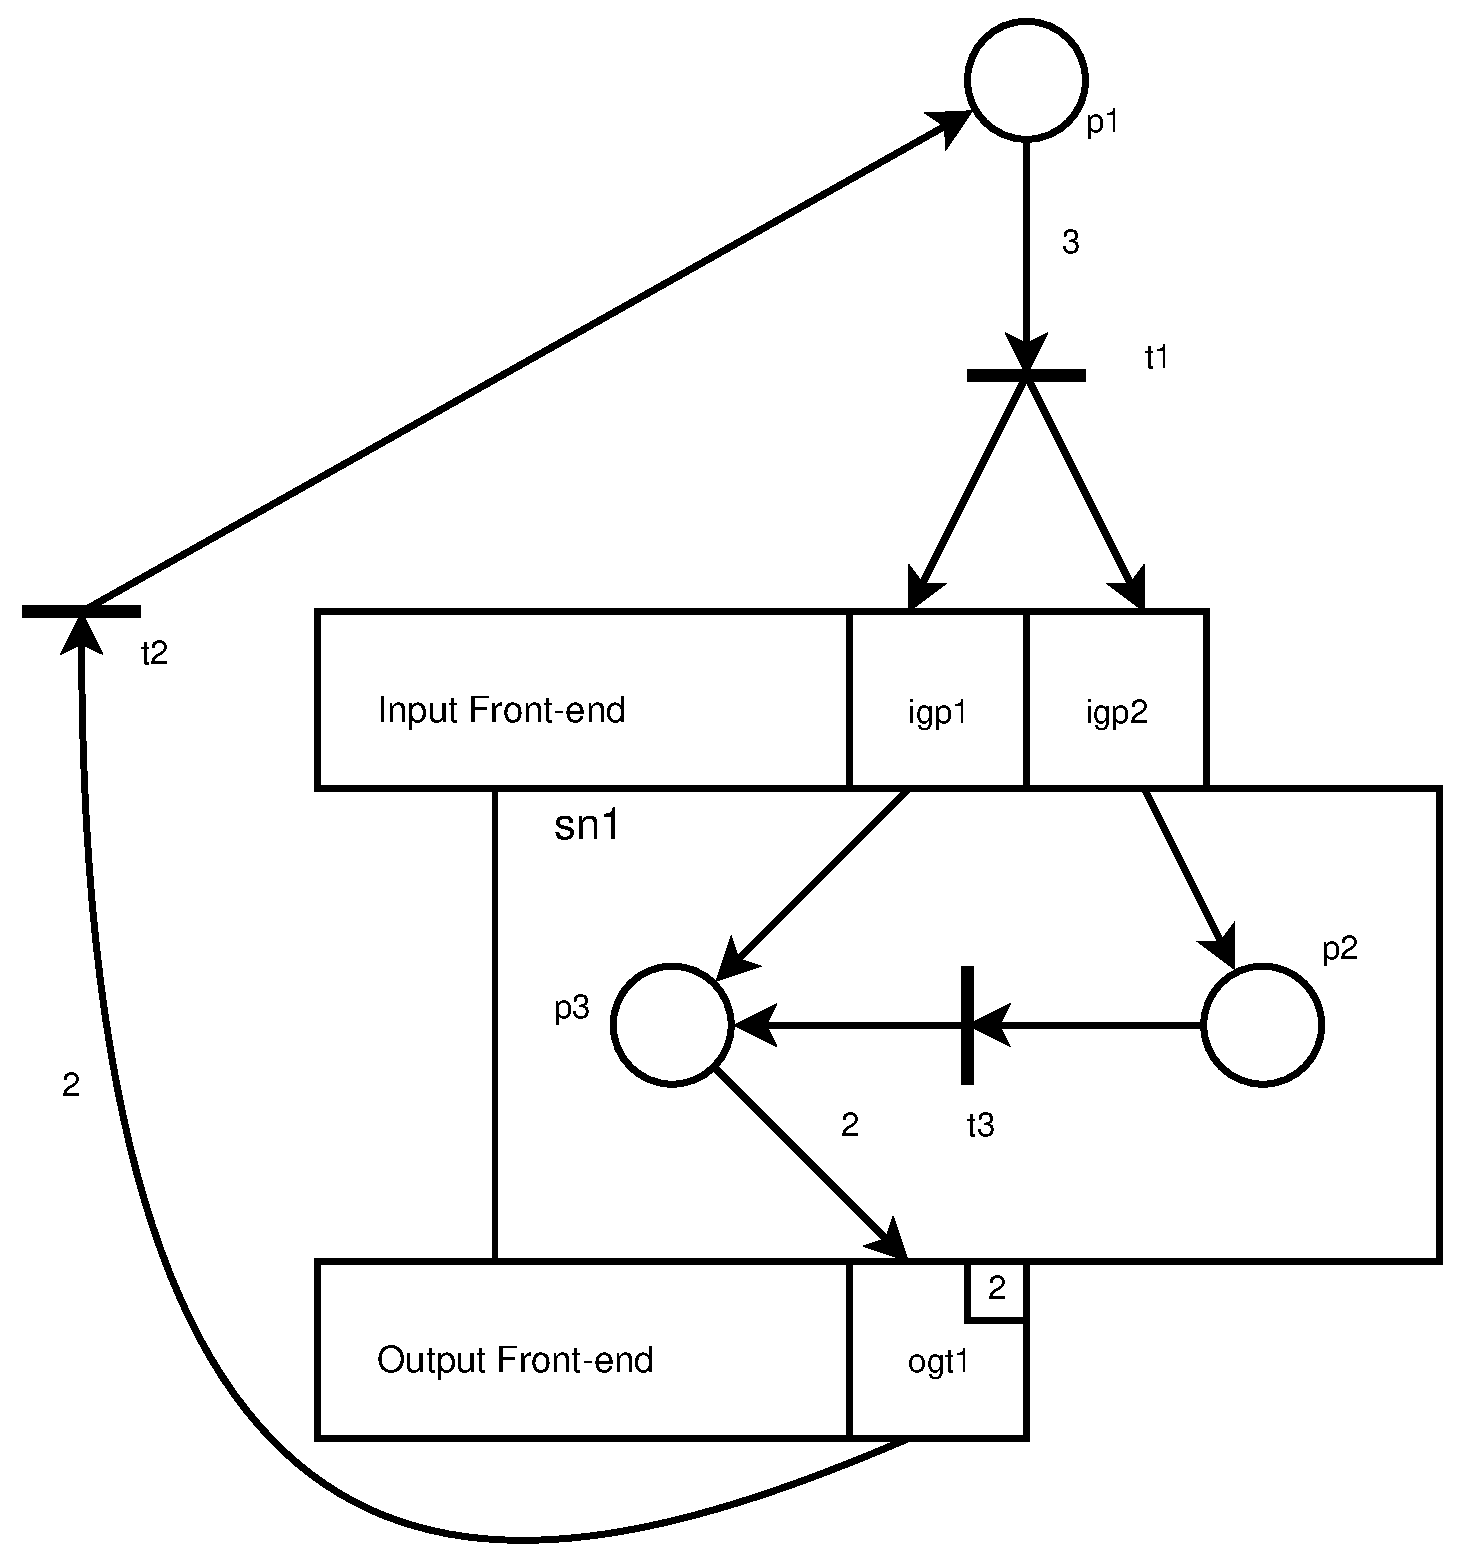
\includegraphics[width=0.60\textwidth]{Figures/PNML-SubredEjemplo1.eps}
\]

...and its PNML representation

\begin{lstlisting}
<subnet id="sn1">
  <interface id="sn1-interface">
    <gate id="igp1" action="input" type="place"/>
    <gate id="igp2" action="input" type="place"/>
    <gate id="ogt1" action="output" type="transition">
      <inscription>
        <text> 2 </text>
      </inscription>
    </gate>
  </interface>
  <content id="sn1-content">
    <place id="p2"/>
    <place id="p3"/>
    <transition id="t3"/>
    <arc id="a2" source="igp2" target="p2"/>
    <arc id="a3" source="igp1" target="p3"/>
    <arc id="a4" source="p3" target="ogt1">
      <inscription>
        <text> 2 </text>
      </inscription>
    </arc>
    <arc id="a5" source="t3" target="p3"/>
    <arc id="a6" source="p2" target="t3"/>
  </content>
</subnet>
<place id="p1"/>
<transition id="t1"/>
<transition id="t2"/>
<arc id="a1" source="p1" target="t1">
  <inscription>
    <text> 3 </text>
  </inscription>
</arc>
<arc id="a2" source="t1" target="igp2"/>
<arc id="a3" source="t1" target="igp1"/>
<arc id="a4" source="ogt1" target="t2">
  <inscription>
    <text> 2 </text>
  </inscription>
</arc>
<arc id="a7" source="t2" target="p1"/>
\end{lstlisting}

The goal is to hide the internal content of the subnet. If we apply XMLEncryption
to the data contained inside the tag \texttt{\textless content\textgreater},\ we will get something like this, depending on the algorithm and key selected for the ciphering.

\begin{lstlisting}
<subnet id="sn1">
  <interface id="sn1-interface">
    <gate id="igp1" action="input" type="place"/>
    <gate id="igp2" action="input" type="place"/>
    <gate id="ogt1" action="output" type="transition">
      <inscription>
        <text> 2 </text>
      </inscription>
    </gate>
  </interface>
  <content id="sn1-content">
    <xenc:EncryptedData xmlns:xenc="http://www.w3.org/2001/04/xmlenc#"  
        Type="http://www.w3.org/2001/04/xmlenc#Element">  
        <xenc:EncryptionMethod  
            Algorithm="http://www.w3.org/2001/04/xmlenc#aes128-cbc"  
            xmlns:xenc="http://www.w3.org/2001/04/xmlenc#" />  
        <xenc:CipherData  
            xmlns:xenc="http://www.w3.org/2001/04/xmlenc#">  
            <xenc:CipherValue  
                xmlns:xenc="http://www.w3.org/2001/04/xmlenc#">  
                  Wr1njyJlYYOM9lAYqcwGCWkw2L4pUjQD2GGVoU9lVZ0wKqHY8y3lGY8FY4i5K
                  3GY8FY4i5K3G8grIe1HRFqe7RtkFiXZgGMeYnQp6oB6ckKp3KFKHVqtucc9rA
                  VzOgC7XAwe61HRFqe6RRVzXjNM9hlVZ0wKqHY8y3l3GY8FY4i5K3G8grIe2xN
                  4u7x7fRtkFiXZgGMeYnQp6oB6ckKp3KFRRVzXjNAtVzOgC7XAw/oe61HRFqe6
                  RRVzXjNMLU5ZgGMeYny8NVPQmUSDX7NRtnR6YnQp6oB6GY8F=
            </xenc:CipherValue>  
        </xenc:CipherData>  
    </xenc:EncryptedData>
  </content>
</subnet>
<place id="p1"/>
<transition id="t1"/>
<transition id="t2"/>
<arc id="a1" source="p1" target="t1">
  <inscription>
    <text> 3 </text>
  </inscription>
</arc>
<arc id="a2" source="t1" target="igp2"/>
<arc id="a3" source="t1" target="igp1"/>
<arc id="a4" source="ogt1" target="t2">
  <inscription>
    <text> 2 </text>
  </inscription>
</arc>
<arc id="a7" source="t2" target="p1"/>
\end{lstlisting} 
 If we try to represent this Petri net we will have the interface of the
 subnet, but the content is a black box.
So it is as follows in the figure:

\begin{figure}[htbp]
\centering
\[
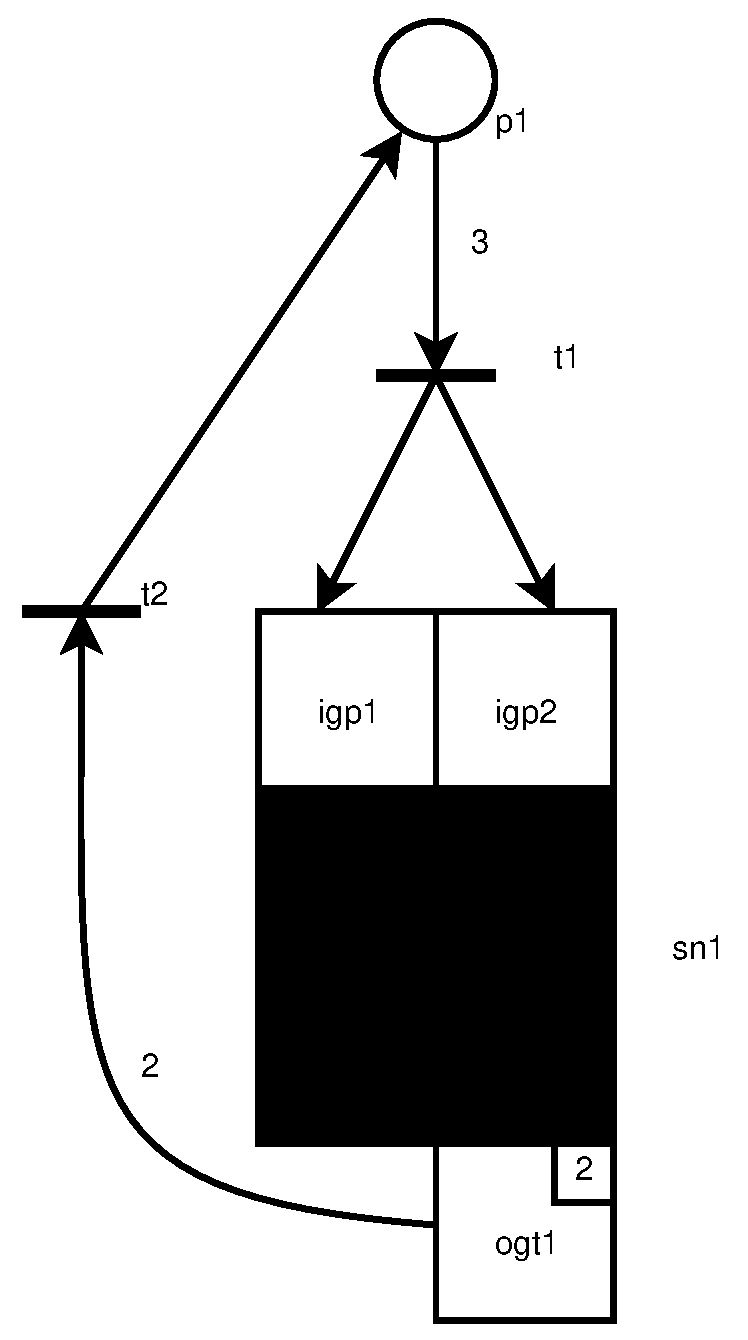
\includegraphics[width=0.40\textwidth]{Figures/XMLENC-SubredEjemplo1.eps}
\]
\rule{35em}{0.5pt}
 \caption{Petri net with hidden subnet}
 \label{fig:XMLENC_SubredEjemplo1} 
\end{figure}

 
\section{Examples}

\subsection{Hidding several subnets}\label{Example several subnets}

One important thing is that I can cipher several subnets of the same Petri
net with distinct options. For example, if there are two subnets for both
two distinct receivers each one of the subnets can be configured in order
to each subnet can be decrypted by its own receiver.

//TODO

\subsection{Critical processes}

//TODO

\section{Conclusions}

As we have seen, one of the applications of subneting Petri nets and represent
them in PNML is that I can apply standard processes based on XML. In this
case, once defined and represented a subnet in PNML, I have apply XMLEncryption in order to hide the internal structure of the subnet.

Actually, there are several options to apply XMLEncryption, such as the algorithm
or the key. The exact election of those option values is responsibility of the Petri net sender. For example:
\begin{itemize}
 \item Maybe both parts (sender and receiver) have a common
set of keys, so they can use it in order to encrypt and decrypt the subnet.
 \item Other common use is that
the key is defined inside the options but it is ciphered itself. If the receiver
have a pair of keys (public and private) and an asymmetrical algorithm (such as Diffie-Hellman or RSA) , the symmetric key can be ciphered by
the sender with the receiver's public key. In this case, only the receiver
can decrypt it using his private key.
\end{itemize}
Other important thing is that several subnets in the same net can be encrypted with different
options. This is used, for example, for  one receiver
to decrypt the subnet addressed to him but no other one.

With the explained in this chapter, the privacy of parts of a Petri net is guarantied.    
 
%\input{Chapters/Chapter6} 
%\input{Chapters/Chapter7} 
% Chapter Template

\chapter{Conclusions} % Main chapter title

\label{Chapter: Conclusions} % Change X to a consecutive number; for referencing this chapter elsewhere, use \ref{Chapter4}

\lhead{Chapter . \emph{Conclusions}} % Change X to a consecutive number; this is for the header on each page - perhaps a shortened title

%\textbf{Intentar que sea un resumen de todo lo tratado, haciendo hincapie en lo aportado y en futuras lineas de investigacion. Que no sea corta. Lo suficientemente larga para que alguien que se lea la tesis pueda recordarla completamente}

Throughout this paper I have enriched Petri nets with definitions and properties. From this initial presentation, have been building a series of elements as a basis for further investigation. We defined subnets, subnets classifications have been studied, we have defined front-ends (interfaces) for those subnets, etc.. From this point is possible a further study of these subnets (their properties, utilities,....)
and the methodological study of securing parts of Petri nets. 

In the first chapter of this thesis I have introduced the research problem.
The nets are represented in a comprehensive way, so that the whole information is visible to everybody. Furthermore, these nets are not prepared to avoid undesired changes or to ensure the authoring of them.

So here is my contribution  to the knowledge: to provide security to a Petri net. The aspects covered by this investigation are:


\begin{itemize}
\item 
to occult a part of the net (or entire). The secret is maintained, and all the information
is stored in the same file, but hidden.
This information is only available to accredited people.
\item to avoid unwanted changes.
Any modification is, at least, detected.\item to authenticate the net (or a part of it). We know who has developed
a Petri net or subnet.
\item to avoid the possibility of supplant other people in the authority of
the Petri net or some of its parts.
\end{itemize}


The next chapter is the state of the art. In this chapter, the literature
about subnets, hiding, encryption, Petri net representation, PNML extensions,
Petri net securing, etc. are grouped and analyzed in order to understand the general knowledge about these topics, related to my objectives. The general conclusions in this part are:
\begin{itemize}
\item There are lots of authors and contents about Petri nets but very few
about subnets.
\item There is no standard way to represent
subnets in a form that is not graphical.
\item Many works studied security using Petri nets, but there is not literature
about security over Petri nets themselves.
\item In particular there is not material on how to hide parts of a Petri nets and either about integrity, authentication or non repudiation.
\end{itemize}
 
Once reviewed the state of the art, I enter into the study of subnets. The main goal is to find a structure of Petri subnets that is easily represented in other formats in addition to graphical mode.

In this chapter I explain how to cut a Petri net into several subnets using the incidence matrix. The method of cutting into two subnets is studied. This method split the incidence matrix into four parts: the subnets per se and two other parts that defined the interaction between this two subnets ($N_1$,
$N_2$, $PIM$ and $TIM$). This will allow us to define the front-end of a subnet in order to abstract is content from the rest of the net.

Once explained subnets, I make a subnet classification. This classification is based on the structure properties. So we can talk about:

\begin{itemize}
\item disjoint subnets, if there are not arcs between the element of the
subnet.
\item macroplaces, if the only way to enter the subnet is from a transition
outside towards a place inside.
\item macrotransitions, if the only way to enter the subnet is from a place
outside towards a transition inside.
\item sinkhole, if there is no arc leaving the subnet.
\item source, if there is no arc entering the subnet
\end{itemize}

Then, one of the main parts of the thesis is studied: the subnet front-end.
It is a very important concept because the rest of the thesis is based on
it: if I define a subnet with its own front-end, I can know its behaviour without the necessity of knowing the internal structure. In this chapter, I introduce the critical concepts of front-end, input and output gates from
places or transitions and attachable net that are going to be used later.

This part of the Petri subnets theory is finished, so I can go on the representation
of this kind of subnets. As one of my goals is to hide parts of a Petri net,
but not erasing information, the main problem is to find a way to represent
a subnet in order to cipher information. From my point of view, the only alternative nowadays to solve this problem is the use of PNML. Other representations
cannot maintain or recover the original information once is hidden.

PNML is a xml standard way to represent Petri nets. But it has a problem:
there is noway to represent subnets. So I have explained a possible PNML extension
that support this kind of information. The key is the definition of several custom xml tags: \texttt{<subnet>}, \texttt{<interface>}, \texttt{<gate>} and \texttt{<content>}. These four tags are enough to my goals. But Petri
nets are a really wide knowledge area. So i don't define a closed PNML extension, but a way for each person to extend it as needed. 

At this moment I have the basis to secure a Petri net (or parts of it). The
next step is the securization itself. The first step is the privacy of the whole
net or only of a part. The technology that I have selected to reach this goal is XMLEncryption. As it is an standard, it is widely extended and
well known. It has de possibility of symmetric and asymmetric ciphering so
the confidentiality of the information is ensured. This method of encryption replace tags in the xml file by encrypted content, only accessible by people
that
knows the right decrypting key. In this case, the tag replaced is \texttt{<content>}, inside
the tag \texttt{<subnet>}. Once this is done only the front-end of the subnet
is exposed, maintaining two properties:

\begin{itemize}
\item The structure of the entire net is not affected, because the interaction
with elements of the subnet is always through the front-end.
\item The information has been not deleted. It is hidden, waiting for somebody
with the correct key.
\item I can change one subnet by another if they have the same front-end,
even though they are ciphered.
\end{itemize} 

The other goals of security are data integrity (not allow unwanted modifications), authentication (know the author or responsible), and non repudiation (nobody
can be supplanted by another one). All of these goals can be achieved by a digital
signature. In this case I my proposition is the use of XMLSignature, that is going to
allow to sign the entire Petri net or only parts of it (the secured ones)
by using XPath expressions. XMLSignature is a standard too, so it has been
widely probed and examined by the community. With XMLSignature the signed content is not replaced.
Instead of that, a new xml element appears in the PNML file with the necessary
information to validate the signature. 

And this is the final stage of this thesis. There several ways to follow in further works. For example:

\begin{itemize}
\item In this thesis I have worked with very basic Petri nets, with only
places, transitions, arcs and weights. This work can be extended to other kind
of Petri nets, such as coloured Petri nets, High level Petri nets, fluid
Petri nets, ...
\item The properties of Petri nets replacing subnets with other subnets can
other field of investigation.
\item The properties of the subnets have not been studied from the point of view
of the behaviour, contemplating markings and evolutions.  
\end{itemize} 
 
% Chapter Template

\chapter{Ejemplos Latex} % Main chapter title

\label{EjemplosLatex} % Change X to a consecutive number; for referencing this chapter elsewhere, use \ref{ChapterX}

\lhead{Ejemplos Latex. \emph{Ejemplos Latex}} % Change X to a consecutive number; this is for the header on each page - perhaps a shortened title

%----------------------------------------------------------------------------------------
%       SECTION 1
%----------------------------------------------------------------------------------------

\section{Codigo XML}


Para poner codigo xml dentro del documento


\begin{lstlisting}
<?xml version="1.0" encoding="utf-8"?>
<xs:schema attributeFormDefault="unqualified" elementFormDefault="qualified"
   xmlns:xs="http://www.w3.org/2001/XMLSchema">
  <xs:element name="points">
    <xs:complexType>
      <xs:sequence>
        <xs:element maxOccurs="unbounded" name="point">
          <xs:complexType>
            <xs:attribute name="x" type="xs:unsignedShort" use="required" />
            <xs:attribute name="y" type="xs:unsignedShort" use="required" />
          </xs:complexType>
        </xs:element>
      </xs:sequence>
    </xs:complexType>
  </xs:element>
</xs:schema>
\end{lstlisting}

\section{varias columnas}

Para poner texto en varias columnas

\begin{multicols}{2}
 Datos en dos columnas fndio fpeowu fpieuwpu piud pqeudp oquewp duqwipud
 pqwudpqwiodu pqwidu pqwidu pqwiud piqwud pqwu dpqwoud pqwod qpwodu qwpdu
 qwpd upou pqowdu wpqo po uqwpod u
\end{multicols}
 

%----------------------------------------------------------------------------------------
%       THESIS CONTENT - APPENDICES
%----------------------------------------------------------------------------------------

\addtocontents{toc}{\vspace{2em}} % Add a gap in the Contents, for aesthetics

\appendix % Cue to tell LaTeX that the following 'chapters' are Appendices

% Include the appendices of the thesis as separate files from the Appendices folder
% Uncomment the lines as you write the Appendices

% Appendix A

\chapter{PNML grammar} % Main appendix title

\label{AppendixA} % For referencing this appendix elsewhere, use \ref{AppendixA}

\lhead{Appendix A. \emph{PNML grammar}} % This is for the header on each page - perhaps a shortened title

The official PNML grammar is available in www.pnml.org. It is written in
RELAX NG format. This are the main parts that I use in this work.

\section{RELAX NG implementation of PNML Core Model}

\begin{lstlisting}[label=grammar_core,caption=RELAX NG implementation of PNML Core Model]
<?xml version="1.0" encoding="UTF-8"?>

<grammar ns="http://www.pnml.org/version-2009/grammar/pnml"
  xmlns="http://relaxng.org/ns/structure/1.0"
  xmlns:a="http://relaxng.org/ns/compatibility/annotations/1.0"
  datatypeLibrary="http://www.w3.org/2001/XMLSchema-datatypes">

  <a:documentation>
    Petri Net Markup Language (PNML) schema.
    RELAX NG implementation of PNML Core Model.

    File name: pnmlcoremodel.rng
    Version: 2009
    (c) 2001-2009
    Michael Weber,
    Ekkart Kindler,
    Christian Stehno, 
    Lom Hillah (AFNOR)
    Revision:
    July 2008 - L.H
  </a:documentation>

  <include href="http://www.pnml.org/version-2009/grammar/anyElement.rng"/>

  <start>
    <ref name="pnml.element"/>
  </start>
  
  <define name="pnml.element">
    <element name="pnml">
      <a:documentation>
        A PNML document consists of one or more Petri nets.
        It has a version.
      </a:documentation>
      <oneOrMore>
        <ref name="pnml.content"/>
      </oneOrMore>
    </element>
  </define>

  <define name="pnml.content">
    <ref name="net.element"/>
  </define>

  <define name="net.element">
    <element name="net">
      <a:documentation>
        A net has a unique identifier (id) and refers to
        its Petri Net Type Definition (PNTD) (type).
      </a:documentation>
      <ref name="identifier.content"/>
      <ref name="nettype.uri"/>
      <a:documentation>
        The sub-elements of a net may occur in any order. 
        A net consists of at least a top-level page which 
        may contain several objects. A net may have a name,
        other labels (net.labels) and tool specific information in any order.   
      </a:documentation>
      <interleave>
        <optional>
          <ref name="Name"/>
        </optional>
        <ref name="net.labels"/>
        <oneOrMore>
          <ref name="page.content"/>
        </oneOrMore>
        <zeroOrMore>
          <ref name="toolspecific.element"/>
        </zeroOrMore>
      </interleave>
    </element>
  </define>

  <define name="identifier.content">
    <a:documentation>
      Identifier (id) declaration shared by all objects in any PNML model.
    </a:documentation>
    <attribute name="id">
      <data type="ID"/>
    </attribute>
  </define>

  <define name="nettype.uri">
    <a:documentation>
      The net type (nettype.uri) of a net should be redefined in the grammar
      for a new Petri net Type.
      An example of such a definition is in ptnet.pntd, the grammar
      for P/T Nets. The following value is a default.
    </a:documentation>
    <attribute name="type">
      <value>http://www.pnml.org/version-2009/grammar/pnmlcoremodel</value> 
    </attribute>
  </define>

  <define name="net.labels">
    <a:documentation>
      A net may have unspecified many labels. This pattern should be used
      within a PNTD to define the net labels.
    </a:documentation>
    <empty/>
  </define>

  <define name="basicobject.content">
    <a:documentation>
      Basic contents for any object of a PNML model.
    </a:documentation>
    <interleave>
      <optional>
        <ref name="Name"/>
      </optional>
      <zeroOrMore>
        <ref name="toolspecific.element"/>
      </zeroOrMore>
    </interleave>  
  </define> 


  <define name="page.content">
    <a:documentation>
      A page has an id. It may have a name and tool specific information.
      It may also have graphical information. It can also have many arbitrary labels.
      Note: according to this definition, a page may contain other pages. 
      All these sub-elements may occur in any order.
    </a:documentation>
    <element name="page">
      <ref name="identifier.content"/>  
      <interleave>
        <ref name="basicobject.content"/>
        <ref name="page.labels"/>
        <zeroOrMore>
          <ref name="netobject.content"/>
        </zeroOrMore>
        <optional>
          <element name="graphics">
            <ref name="pagegraphics.content"/>
          </element>
        </optional>
      </interleave> 
    </element>
  </define>

  <define name="netobject.content">
    <a:documentation>
      A net object is either a page, a node or an arc. 
      A node is a place or a transition, a reference place of
      a reference transition.
    </a:documentation>
    <choice>     
      <ref name="page.content"/>      
      <ref name="place.content"/>  
      <ref name="transition.content"/>    
      <ref name="refplace.content"/>
      <ref name="reftrans.content"/>
      <ref name="arc.content"/>
    </choice>
  </define>

  <define name="page.labels">
    <a:documentation>
      A page may have unspecified many labels. This pattern should be used
      within a PNTD to define new labels for the page concept.
    </a:documentation>
    <empty/>
  </define>

  <define name="place.content">
    <a:documentation>
      A place may have several labels (place.labels) and the same content 
      as a node.
    </a:documentation>
    <element name="place">
      <ref name="identifier.content"/>
      <interleave>
        <ref name="basicobject.content"/>
        <ref name="place.labels"/>
        <ref name="node.content"/>
      </interleave>
    </element>
  </define>

  <define name="place.labels">
    <a:documentation>
      A place may have arbitrary many labels. This pattern should be used
      within a PNTD to define the place labels.
    </a:documentation>
    <empty/>
  </define>

  <define name="transition.content">
    <a:documentation>
      A transition may have several labels (transition.labels) and the same 
      content as a node.
    </a:documentation>
    <element name="transition">
      <ref name="identifier.content"/>    
      <interleave>
        <ref name="basicobject.content"/>
        <ref name="transition.labels"/>
        <ref name="node.content"/>
      </interleave>
    </element>
  </define>

  <define name="transition.labels">
    <a:documentation>
      A transition may have arbitrary many labels. This pattern should be 
      used within a PNTD to define the transition labels.
    </a:documentation>
    <empty/>
  </define>

  <define name="node.content">
    <a:documentation>
      A node may have graphical information.
    </a:documentation>    
    <optional>
      <element name="graphics">
        <ref name="nodegraphics.content"/>
      </element>
    </optional>  
  </define>

  <define name="reference">
    <a:documentation>
      Here, we define the attribute ref including its data type.
      Modular PNML will extend this definition in order to change
      the behavior of references to export nodes of module instances.
    </a:documentation>
    <attribute name="ref">
      <data type="IDREF"/>
    </attribute>
  </define>

  <define name="refplace.content">
    <a:documentation>
      A reference place is a reference node.
    </a:documentation>
    <a:documentation>
      Validating instruction: 
      - _ref_ MUST refer to _id_ of a reference place or of a place.
      - _ref_ MUST NOT refer to _id_ of its reference place element.
      - _ref_ MUST NOT refer to a cycle of reference places.
    </a:documentation>
    <element name="referencePlace">
      <ref name="refnode.content"/>
    </element>
  </define>

  <define name="reftrans.content">
    <a:documentation>
      A reference transition is a reference node.
    </a:documentation>
    <a:documentation>
      Validating instruction: 
      - The reference (ref) MUST refer to a reference transition or to a 
      transition.
      - The reference (ref) MUST NOT refer to the identifier (id) of its
      reference transition element.
      - The reference (ref) MUST NOT refer to a cycle of reference transitions.
    </a:documentation>
    <element name="referenceTransition">
      <ref name="refnode.content"/>
    </element>
  </define>

  <define name="refnode.content">
    <a:documentation>
      A reference node has the same content as a node.
      It adds a reference (ref) to a (reference) node.
    </a:documentation>
    <ref name="identifier.content"/>
    <ref name="reference"/>
    <ref name="basicobject.content"/>
    <ref name="node.content"/>  
  </define>

  <define name="arc.content">
    <a:documentation>
      An arc has a unique identifier (id) and
      refers both to the node's id of its source and 
      the node's id of its target.
      In general, if the source attribute refers to a place, 
      then the target attribute refers to a transition and vice versa.
    </a:documentation>
    <element name="arc">
      <ref name="identifier.content"/>
      <attribute name="source">
        <data type="IDREF"/>
      </attribute>
      <attribute name="target">
        <data type="IDREF"/>
      </attribute>
      <a:documentation>
        The sub-elements of an arc may occur in any order.
        An arc may have a name, graphical and tool specific information.
        It may also have several labels.
      </a:documentation>
      <interleave>
        <optional>
          <ref name="Name"/>
        </optional>
        <ref name="arc.labels"/>
        <optional>
          <element name="graphics">
            <ref name="edgegraphics.content"/>
          </element>
        </optional>
        <zeroOrMore>
          <ref name="toolspecific.element"/>
        </zeroOrMore>
      </interleave>
    </element>
  </define>

  <define name="arc.labels">
    <a:documentation>
      An arc may have arbitrary many labels. This pattern should be used
      within a PNTD to define the arc labels.
    </a:documentation>
    <empty/>
  </define>

  <define name="pagegraphics.content">
    <a:documentation>
      A page graphics is actually a node graphics
    </a:documentation>
    <ref name="nodegraphics.content"/> 
  </define>

  <define name="nodegraphics.content">
    <a:documentation>
      The sub-elements of a node's graphical part occur in any order.
      At least, there may be one position element.
      Furthermore, there may be a dimension, a fill, and a line element.
    </a:documentation>
    <interleave>
      <ref name="position.element"/>
      <optional>
        <ref name="dimension.element"/>
      </optional>
      <optional>
        <ref name="fill.element"/>
      </optional>
      <optional>
        <ref name="line.element"/>
      </optional>
    </interleave>
  </define>

  <define name="edgegraphics.content">
    <a:documentation>
      The sub-elements of an arc's graphical part occur in any order.
      There may be zero or more position elements.
      Furthermore, there may be a line element.
    </a:documentation>
    <interleave>
      <zeroOrMore>
        <ref name="position.element"/>
      </zeroOrMore>
      <optional>
        <ref name="line.element"/>
      </optional>
    </interleave>
  </define>

  <define name="simpletext.content">
    <a:documentation>
      This definition describes the contents of simple text labels
      without graphics.
    </a:documentation>
    <optional>
      <element name="text">
        <a:documentation>
          A text should have a value. 
          If not, then there must be a default.
        </a:documentation>
        <text/>
      </element>
    </optional>
  </define>

  <define name="annotationstandard.content">
    <a:documentation>
      The definition annotationstandard.content describes the 
      standard contents of an annotation.
      Each annotation may have graphical or tool specific information.
    </a:documentation>
    <interleave>
      <optional>
        <element name="graphics">
          <ref name="annotationgraphics.content"/>
        </element>
      </optional>
      <zeroOrMore>
        <ref name="toolspecific.element"/>
      </zeroOrMore>
    </interleave>
  </define>

  <define name="simpletextlabel.content">
    <a:documentation>
      A simple text label is an annotation to a net object containing 
      arbitrary text.
      Its sub-elements occur in any order.
      A simple text label behaves like an attribute to a net object.
      Furthermore, it contains the standard annotation contents which 
      basically defines the graphics of the text.
    </a:documentation>
    <interleave>
      <ref name="simpletext.content"/>
      <ref name="annotationstandard.content"/>
    </interleave>
  </define>

  <define name="Name">
    <a:documentation>
      Label definition for a user given name of an 
      element.
    </a:documentation>
    <element name="name">
      <ref name="simpletextlabel.content"/>
    </element>
  </define>

  <define name="annotationgraphics.content">
    <a:documentation>
      An annotation's graphics part requires an offset element describing
      the offset the center point of the surrounding text box has to
      the reference point of the net object on which the annotation occurs.
      Furthermore, an annotation's graphic element may have a fill, a line, 
      and font element.
    </a:documentation>
    <ref name="offset.element"/>
    <interleave>
      <optional>
        <ref name="fill.element"/>
      </optional>
      <optional>
        <ref name="line.element"/>
      </optional>
      <optional>
        <ref name="font.element"/>
      </optional>
    </interleave>
  </define>

  <define name="position.element">
    <a:documentation>
      A position element describes Cartesian coordinates.
    </a:documentation>
    <element name="position">
      <ref name="coordinate.attributes"/>
    </element>
  </define>

  <define name="offset.element">
    <a:documentation>
      An offset element describes Cartesian coordinates.
    </a:documentation>
    <element name="offset">
      <ref name="coordinate.attributes"/>
    </element>
  </define>

  <define name="coordinate.attributes">
    <a:documentation>
      The coordinates are decimal numbers and refer to an appropriate 
      xy-system where the x-axis runs from left to right and the y-axis
      from top to bottom.
    </a:documentation>
    <attribute name="x">
      <data type="decimal"/>
    </attribute>
    <attribute name="y">
      <data type="decimal"/>
    </attribute>
  </define>

  <define name="dimension.element">
    <a:documentation>
      A dimension element describes the width (x coordinate) and height 
      (y coordinate) of a node.  
      The coordinates are actually positive decimals.
    </a:documentation>
    <element name="dimension">
      <attribute name="x">
        <ref name="positiveDecimal.content"/>
      </attribute>
      <attribute name="y">
        <ref name="positiveDecimal.content"/>
      </attribute>
    </element>
  </define>

  <define name="positiveDecimal.content" ns="http://www.w3.org/2001/XMLSchema-datatypes">
    <a:documentation>
      Definition of a restricted positive decimals domain with a total digits 
      number of 4 and 1 fraction digit. Ranges from 0 to 999.9
    </a:documentation>
    <data type='decimal'>
      <param name='totalDigits'>4</param>
      <param name='fractionDigits'>1</param>
      <param name='minExclusive'>0</param>
    </data>
  </define>

  <define name="fill.element">
    <a:documentation>
      A fill element describes the interior colour, the gradient colour,
      and the gradient rotation between the colors of an object.  If an
      image is available the other attributes are ignored.
    </a:documentation>
    <element name="fill">
      <optional>
        <attribute name="color">
          <ref name="color.type"/>
        </attribute>
      </optional>
      <optional>
        <attribute name="gradient-color">
          <ref name="color.type"/>
        </attribute>
      </optional>
      <optional>
        <attribute name="gradient-rotation">
          <choice>
            <value>vertical</value>
            <value>horizontal</value>
            <value>diagonal</value>
          </choice>
        </attribute>
      </optional>
      <optional>
        <attribute name="image">
          <data type="anyURI"/>
        </attribute>
      </optional>
    </element>
  </define>

  <define name="line.element">
    <a:documentation>
      A line element describes the shape, the colour, the width, and the 
      style of an object.
    </a:documentation>
    <element name="line">
      <optional>
        <attribute name="shape">
          <choice>
            <value>line</value>
            <value>curve</value>
          </choice>
        </attribute>
      </optional>
      <optional>
        <attribute name="color">
          <ref name="color.type"/>
        </attribute>
      </optional>
      <optional>
        <attribute name="width">
          <ref name="positiveDecimal.content"/>
        </attribute>
      </optional>
      <optional>
        <attribute name="style">
          <choice>
            <value>solid</value>
            <value>dash</value>
            <value>dot</value>
          </choice>
        </attribute>
      </optional>
    </element>
  </define>

  <define name="color.type">
    <a:documentation>
      This describes the type of a color attribute. Actually, this comes
      from the CSS2 (and latest versions) data type system.
    </a:documentation>
    <text/>
  </define>

  <define name="font.element">
    <a:documentation>
      A font element describes several font attributes, the decoration, 
      the alignment, and the rotation angle of an annotation's text.
      The font attributes (family, style, weight, size) should be conform
      to the CSS2 and latest versions data type system.
    </a:documentation>
    <element name="font">
      <optional>
        <attribute name="family">
          <text/>  <!-- actually, CSS2 and latest versions font-family -->
        </attribute>
      </optional>
      <optional>
        <attribute name="style">
          <text/>  <!-- actually, CSS2 and latest versions font-style -->
        </attribute>
      </optional>
      <optional>
        <attribute name="weight">
          <text/>  <!-- actually, CSS2 and latest versions font-weight -->
        </attribute>
      </optional>
      <optional>
        <attribute name="size">
          <text/>  <!-- actually, CSS2 and latest versions font-size -->
        </attribute>
      </optional>
      <optional>
        <attribute name="decoration">
          <choice>
            <value>underline</value>
            <value>overline</value>
            <value>line-through</value>
          </choice>
        </attribute>
      </optional>
      <optional>
        <attribute name="align">
          <choice>
            <value>left</value>
            <value>center</value>
            <value>right</value>
          </choice>
        </attribute>
      </optional>
      <optional>
        <attribute name="rotation">
          <data type="decimal"/>
        </attribute>
      </optional>
    </element>
  </define>

  <define name="toolspecific.element">
    <a:documentation>
      The tool specific information refers to a tool and its version.
      The further substructure is up to the tool.
    </a:documentation>
    <element name="toolspecific">
      <attribute name="tool">
        <text/>
      </attribute>
      <attribute name="version">
        <text/>
      </attribute>
      <zeroOrMore>
        <ref name="anyElement"/>
      </zeroOrMore>
    </element>
  </define>
  
</grammar>
\end{lstlisting}







\newpage

\section{RELAX NG implementation of Petri Net Type Definition for Place/Transition nets}

\begin{lstlisting}[label=grammar_place_transitions,caption=RELAX NG implementation of PNTD for Place/Transition nets]
<?xml version="1.0" encoding="UTF-8"?>

<grammar ns="http://www.pnml.org/version-2009/grammar/pnml"
  xmlns="http://relaxng.org/ns/structure/1.0"
  xmlns:a="http://relaxng.org/ns/compatibility/annotations/1.0"> 

  <a:documentation>
    RELAX NG implementation of Petri Net Type Definition for Place/Transition nets.
    This PNTD re-defines the value of nettype.uri for P/T nets.
    
    File name: ptnet.pntd
    Version: 2009
    (c) 2007-2009
    Lom Hillah (AFNOR)
    Revision:
    July 2008 - L.H
  </a:documentation>

  <a:documentation>
    The PT Net type definition.
    This document also declares its namespace.
    All labels of this Petri net type come from the Conventions document.
    The use of token graphics as tool specific feature is possible.
  </a:documentation>

  <include href="http://www.pnml.org/version-2009/grammar/conventions.rng"/>
  
  <!--
  <include href="http://www.pnml.org/version-2009/grammar/pnmlextensions.rng"/>
    We do not need to include this, because the pnmlcoremodel.rng covers any
    toolspecific extension.
  -->
  
  <include href="http://www.pnml.org/version-2009/grammar/pnmlcoremodel.rng"/>
  
  <define name="nettype.uri" combine="choice">
    <a:documentation>
      The URI value for the net type attribute, 
      declaring the type of P/T nets.
    </a:documentation>
    <attribute name="type">    
      <value>http://www.pnml.org/version-2009/grammar/ptnet</value>   
    </attribute>
  </define>

  
  <define name="PTMarking">
    <a:documentation>
      Label definition for initial marking in nets like P/T-nets.
      <contributed>Michael Weber</contributed>
      <date>2003-06-16</date>
      <reference>
        W. Reisig: Place/transition systems. In: LNCS 254. 1987.
      </reference>
    </a:documentation>
    <element name="initialMarking">
      <ref name="nonnegativeintegerlabel.content"/>
    </element>
  </define>

  <define name="PTArcAnnotation">
    <a:documentation>
      Label definition for arc inscriptions in P/T-nets.
      <contributed>Michael Weber, AFNOR</contributed>
      <date>2003-06-16</date>
      <reference>
        W. Reisig: Place/transition systems. In: LNCS 254. 1987.
      </reference>
    </a:documentation>
    <element name="inscription">
      <ref name="positiveintegerlabel.content"/>
    </element>
  </define>

  <define name="place.labels" combine="interleave">
    <a:documentation>
      A place of a P/T net may have an initial marking.
    </a:documentation> 
    <optional><ref name="PTMarking"/></optional>
  </define>

  <define name="arc.labels" combine="interleave">
    <a:documentation>
      An arc of a P/T net may have an inscription.
    </a:documentation>
    <optional><ref name="PTArcAnnotation"/></optional>
  </define>

</grammar>
\end{lstlisting}

%\input{Appendices/AppendixB}
%\input{Appendices/AppendixC}

\addtocontents{toc}{\vspace{2em}} % Add a gap in the Contents, for aesthetics

\backmatter

%----------------------------------------------------------------------------------------
%       BIBLIOGRAPHY
%----------------------------------------------------------------------------------------

\label{Bibliography}

\lhead{\emph{Bibliography}} % Change the page header to say "Bibliography"

\bibliographystyle{unsrtnat} % Use the "unsrtnat" BibTeX style for formatting the Bibliography

\bibliography{Bibliography} % The references (bibliography) information are stored in the file named "Bibliography.bib"
\textbf{Faltan las referencias de paginas web}
\end{document}  
